\documentclass{beamer}
\usepackage{graphicx}

\usepackage{url}

\usepackage{amsmath}
\usepackage{amssymb}
\usepackage{xkeyval}

\usepackage{../macros/mytikz}
\usepackage{listings}
\lstset{mathescape}

\usepgflibrary{shapes}
\usepackage{stmaryrd}

\usepackage{../macros/basics}
\usepackage{../macros/basics-slides}
%\usepackage{../macros/mmt_listings}
\usepackage{../macros/twelf-math}

\usepackage{../macros}
\usepackage{local}


\newcommand{\lf}{\mathit{LF}}
\newcommand{\kity}{\mathit{type}}


\renewcommand{\emph}[1]{\alert{#1}}

%\setbeamertemplate{headline}{\small\hfill\insertsection \hfill\hbox{}}

\begin{document}

\title{Knowledge Representation and Processing}
\author{Florian Rabe (for a course given with Michael Kohlhase)}
\institute{Computer Science, University Erlangen-N\"urnberg, Germany}
\date{2023}
\begin{frame}
    \titlepage
\end{frame}

%%%%%%%%%%%%%%%%%%%%%%%%%%%%%%%%%%%%%%%%%%%%%
\part{Introduction}
\section{Administrative Information}

\begin{frame}\frametitle{Format}
\begin{blockitems}{Zoom}
\item lectures and exercises in person --- if we have a room
\item zoom for now
\item interaction strongly encouraged
 \lec{We don't want to lecture ---}
 \lec{we want to have a conversation during which you learn}
\item make use of zoom
 \begin{itemize}
 \item use reactions to say yes no, ask for break etc.
 \item feel free to annotate my slides
 \item talk in the chat
 \end{itemize}
\end{blockitems}

\begin{blockitems}{Recordings}
\item maybe prerecorded video lectures or recorded zoom meeting
\item to be decided along the way
\end{blockitems}
\end{frame}


\begin{frame}\frametitle{Background}
\begin{blockitems}{Instructors}
\item Prof. Dr. Michael Kohlhase \lec{Professor of Knowledge Representation and Processing}
\item PD Dr. Florian Rabe \lec{same research group}
\end{blockitems}

\begin{blockitems}{Course}
\item This course is given for the second time
\item First time was a little bit of an experiment
  \lec{polishing and revising the materials this year}
\item To become signature course of our research group \lec{same name!}
\end{blockitems}
\end{frame}

\begin{frame}\frametitle{Prerequisites}
\begin{blockitems}{Required}
\item basic knowledge about formal languages, context-free grammars
 \lec{but we'll do a quick revision here}
\end{blockitems}

\begin{blockitems}{Helpful}
\item Algorithms and Data Structures
 \lec{mostly as a contrast to this lecture}
\item Basic logic
 \lec{we'll revise it slightly differently here}
\item all other courses
 \lec{as examples of how knowledge pervades all of CS}
\end{blockitems}

\begin{blockitems}{General}
\item Curiosity \lec{this course is a bit unusual}
\item Interest in big picture \lec{this course touches on lots of things from all over CS}
\end{blockitems}
\end{frame}

\begin{frame}\frametitle{Examination and Grading}
\begin{blockitems}{Suggestion}
\item grade determined by single exam
\item oral, 30 minutes
\item exercises indirectly graded through conversation during exam
\end{blockitems}

\begin{blockitems}{Exam-relevant}
\item anything mentioned in notes
\item anything discussed in lectures
\item anything done in exercises
\end{blockitems}
\lec{neither is a superset of the other!}
\end{frame}

\begin{frame}\frametitle{Materials and Exam-Relevance}
\begin{blockitems}{Textbook}
\item does not exist
\item normal for research-near specialization courses
\end{blockitems}

\begin{blockitems}{Notes}
\item textbook-style but not as comprehensive
\item developed along the way
\item systematic write-up, not necessarily in lecture order
\end{blockitems}

\begin{blockitems}{Slides}
\item not comprehensive
\item used as visual aid, conversation starters
\end{blockitems}
\end{frame}

\begin{frame}\frametitle{Communication}
\begin{blockitems}{Open for questions}
\item open door policy in our offices
\item always room for questions during lectures
\item for personal questions, contact me during/after lecture
\item forum at studon
\end{blockitems}

\begin{blockitems}{Materials}
\item notes and slides are at: \url{https://github.com/florian-rabe/Teaching/tree/master/WuV}
\item currently last year's version, will change throughout the semester
\lec{you can read ahead, but maybe don't print everything right away}
\item pull requests and issues welcome
\end{blockitems}
\end{frame}

\begin{frame}\frametitle{Exercises}
\begin{blockitems}{Learning Goals}
\item Get acquainted with state of the art of practice
\item Try out real tools
\end{blockitems}

\begin{blockitems}{Homeworks}
\item one major project as running example
\item homeworks building on each other
\end{blockitems}
\lec{build one large knowledge-based system}
\lec{details on later slides}
\end{frame}

\section{Overview and Essential Concepts}

\begin{frame}\frametitle{Representation and Processing}
Common pairs of concepts:
\begin{center}
\begin{tabular}{l|l}
Representation & Processing \\
\hline
Static & Dynamic \\
Situation & Change \\
Be & Become \\
Data Structures & Algorithms \\
Set & Function \\
State & Transition \\
Space & Time
\end{tabular}
\end{center}
\end{frame}

\begin{frame}\frametitle{Data and Knowledge}
$2\times 2$ key concepts
\begin{center}
\begin{tabular}{l|l}
Syntax & Data \\
\hline
Semantics & Knowledge
\end{tabular}
\end{center}

\begin{itemize}
\item Data: any object that can be stored in a computer\\
 Example: $((49.5739143, 11.0264941), "2020-04-21T16:15:00CEST")$
\item Syntax: a system of rules that describes which data is \textbf{well-formed}\\
 Example: ``a pair of (a pair of two IEEE double precision floating point numbers) and a string encoding of a time stamp''
\item Semantics: system of rules that determines the meaning of well-formed data
\item Knowledge: combination of some data with its syntax and semantics
\end{itemize}
\end{frame}

\begin{frame}\frametitle{Knowledge is Elusive}
Representation of key concepts 
\begin{itemize}
 \item Data: using primitive objects
  \lec{implemented as bits, bytes, strings, records, arrays, \ldots}
 \item Syntax: (context-free) grammars, (context-sensitive) type systems
  \lec{implemented as inductive data structures}
 \item Semantics: functions for evaluation, interpretation, of well-formed data
  \lec{implemented as recursive algorithms on the syntax}
 \item Knowledge: elusive
  \lec{emerges from applying and interacting with the semantics}
\end{itemize}
\end{frame}

\begin{frame}\frametitle{Semantics as Translation}
\begin{itemize}
\item Knowledge can be captured by a higher layer of syntax
\item Then semantics is translation into syntax
\end{itemize}

\begin{center}
\begin{tabular}{l|l|l}
Data syntax & Semantics function & Knowledge syntax \\
\hline
SPARQL query & evaluation & result set \\
SQL query & evaluation & result table \\
program & compiler & binary code \\
program expression & interpreter & result value \\ 
logical formula & interpretation in a model & mathematical object \\
HTML document & rendering & graphics context
\end{tabular}
\end{center}
\end{frame}

\begin{frame}\frametitle{Heterogeneity of Data and Knowledge}
\begin{itemize}
\item Capturing knowledge is difficult
\item Many different approaches to semantics
 \begin{itemize}
  \item fundamental formal and methodological differences
  \item often captured in different fields, conferences, courses, languages, tools
 \end{itemize}
\item Data formats equally heterogeneous
 \begin{itemize}
 \item ontologies
 \item programs
 \item logical proofs
 \item databases
 \item documents
 \end{itemize}
\end{itemize}
\end{frame}

\begin{frame}\frametitle{Challenges of Heterogeneity}
\begin{blockitems}{Challenges}
\item collaboration across communities
\item translation across languages
\item conversion between data formats
\item interoperability across tools
\end{blockitems}

\begin{blockitems}{Sources of problems}
\item interoperability across formats/tools major source of
 \begin{itemize}
 \item complexity
 \item bugs
 \end{itemize}
\item friction in project team due to differing preferences, expertise
\item difficult choice between languages/tools with competing advantages
\begin{itemize}
 \item reverting choices difficult, costly
 \item maintaining legacy choices increases complexity
\end{itemize}
\end{blockitems}
\end{frame}

\begin{frame}\frametitle{Aspects of Knowledge}
\begin{itemize}
\item Tetrapod model of knowledge
  \lec{active research by our group}
\item classifies approaches to knowledge into five aspects
\end{itemize}

\begin{center}
\begin{tabular}{lll}
Aspect & KRLs (examples) & KPTs (examples) \\
\hline
ontologization & ontology languages (OWL), description logics (ALC) & reasoners, SPARQL engines (Virtuoso) \\
concretization & relational databases (SQL, JSON) & databases (MySQL, MongoDb) \\
computation & programming languages (C) & interpreters, compilers (gcc) \\
deduction & logics (HOL) & theorem provers (Isabelle) \\
narration & document languages (HTML, LaTeX) & editors, viewers
\end{tabular}
\end{center}
\end{frame}

\begin{frame}\frametitle{Relations between the Aspects}
Ontology is distinguished: capture the knowledge that the other four aspects share

\begin{center}
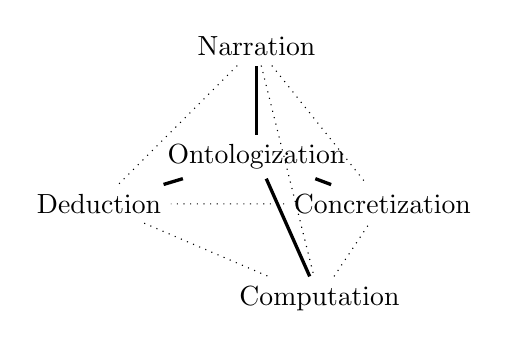
\begin{tikzpicture}[scale=4]
  \node (center) at (0,.15) {Ontologization};
  \node (left) at (.2,-.3) {Computation};
  \node (right) at (.4,0) {Concretization};
  \node (back) at (-.5,0) {Deduction};
  \node (up) at (0,.5) {Narration};

  \draw[very thick] (center) -- (left);
  \draw[very thick] (center) -- (right);
  \draw[very thick] (center) -- (back);
  \draw[very thick] (center) -- (up);
  \draw[dotted] (left) -- (right) -- (back) -- (left);
  \draw[dotted] (up) -- (left);
  \draw[dotted] (up) -- (right);
  \draw[dotted] (up) -- (back);
\end{tikzpicture}
\end{center}
\end{frame}

\begin{frame}\frametitle{Complementary Advantages of the Aspects}
\begin{center}
\footnotesize
\begin{tabular}{|l|llp{2.1cm}l|}\hline
Aspect & objects & \multicolumn{3}{c|}{characteristic} \\
       &         & advantage & joint advantage of the other aspects & application \\\hline
ded. & formal proofs & correctness & ease of use & verification \\
comp. & programs & efficiency & well-definedness & execution\\
concr. & concrete objects & queriability & abstraction & storage/retrieval\\
narr. & texts & flexibility & formal semantics & human understanding\\\hline
\end{tabular}
\medskip

\begin{tabular}{|l|l|}\hline
Aspect pair & characteristic advantage \\\hline
ded./comp.  & rich meta-theory \\
narr./conc. & simple languages \\\hline
ded./narr.  & theorems and proofs \\
comp./conc. & normalization \\\hline
ded./conc.  & decidable well-definedness \\
comp./narr. & Turing completeness \\\hline
\end{tabular}
\end{center}
\end{frame}

\begin{frame}\frametitle{Structure of the Course}
\begin{blockitems}{Aspect-independent parts}
\item shared characteristics
\item general methods
\end{blockitems}

\begin{blockitems}{Aspects-specific parts}
\item one part for each aspect
\item high-level overview of state of the art
\item focus on comparison/evaluation of the aspect-specific results
\end{blockitems}
\end{frame}

\begin{frame}\frametitle{Structure of the Exercises}
\begin{blockitems}{One major project}
\item representative for a project that a CS graduate might be put in charge of
\item challenging heterogeneous data and knowledge
\item requires integrating/combining different languages, tools
\end{blockitems}
\lec{unique opportunity in this course because knowledge is everywhere}

\begin{blockitems}{Concrete project}
\item develop a campo/studnon-style KRP system for a university
\item lots of heterogeneous knowledge
 \begin{itemize}
 \item course and program descriptions
 \item legal texts
 \item websites
 \item grade tables
 \item code to generate diplomas
 \end{itemize} 
\item build a functional system applying the lessons of the course
\lec{we'll see how far we get --- priority is learning}
\end{blockitems}
\end{frame}


%%%%%%%%%%%%%%%%%%%%%%%%%%%%%%%%%%%%%%%%%%%%%
\part{Ontologies}
\section{Ontological Knowledge}

\begin{frame}\frametitle{Components of an Ontology}
8 main declarations
\begin{itemize}
 \item \textbf{individual} --- concrete objects that exist in the real world, e.g., "Florian Rabe" or "WuV"
 \item \textbf{concept} --- abstract groups of individuals, e.g., "instructor" or "course"
 \item \textbf{relation} --- binary relations between two individuals, e.g., "teaches"
 \item \textbf{properties} --- binary relations between an individuals and a concrete value (a number, a date, etc.), e.g., "has-credits"
 \item \textbf{concept assertions} --- the statement that a particular individual is an instance of a particular concept
 \item \textbf{relation assertions} --- the statement that a particular relation holds about two individuals
 \item \textbf{property assertions} --- the statement that a particular individual has a particular value for a particular property
 \item \textbf{axioms} --- statements about relations between concepts, e.g., "instructor" $\sqsubseteq$ "person"
\end{itemize}
\end{frame}

\begin{frame}\frametitle{Divisions of an Ontology}
\begin{blockitems}{Abstract vs. concrete}
 \item TBox: concepts, relations, properties, axioms
  \lec{everything that does not use individuals}
 \item ABox: individuals and assertions
\end{blockitems}

\begin{blockitems}{Named vs. unnamed}
 \item Signature: individuals, concepts, relations, properties \lec{together called entities or resources}
 \item Theory: assertions, axioms
\end{blockitems}
\end{frame}

\begin{frame}\frametitle{Comparison of Terminology}
\begin{center}
\tiny
\begin{tabular}{l|llll|l}
 Here       & OWL      & Description logics & ER model & UML & semantics via logics\\
\hline
 individual & instance & individual & entity & object, instance & constant\\
 concept    & class    & concept &  entity-type & class & unary predicate\\
 relation   & object property & role & role & association & binary predicate \\
 property   & data property   & (not common) & attribute & field of base type & binary predicate\\
\end{tabular}
\medskip

\begin{tabular}{l|ll}
 domain & individual & concept \\
\hline
type theory, logic & constant, term & type \\
set theory  & element & set \\
database    & row & table \\
philosophy\footnote{as in \url{https://plato.stanford.edu/entries/object/}} & object & property \\
grammar & proper noun & common noun \\
\end{tabular}
\end{center}
\end{frame}

\begin{frame}\frametitle{Ontologies as Sets of Triples}
General idea:
\begin{itemize}
\item Turn everything into a relation/property assertion
\item Represent ontologies as sets of subject-predicate-object triples
\item Obtain efficient representation of ontologies using RDF and RDFS
\end{itemize}

\begin{center}
\begin{tabular}{l|lll}
Assertion & \multicolumn{3}{c}{Triple} \\
          & Subject & Predicate & Object \\
\hline
entities           & \multicolumn{3}{|l}{recover from what's mentioned in assertions} \\
concept assertion  & "Florian Rabe" & \texttt{is-a} & "instructor" \\
relation assertion & "Florian Rabe" & "teaches" & "WuV" \\
property assertion & "WuV" & "has credits" & 7.5 \\
axiom              & \multicolumn{3}{|l}{only some special cases work, e.g.,}\\
\tb subconcept axiom & "instructor" & \texttt{subClassOf} & "person"\\
\end{tabular}
\end{center}
\end{frame}

\begin{frame}\frametitle{Special Entities}
RDF and RDFS define special entities for use in ontologies:
\begin{itemize}
 \item "rdfs:Resource": concept of which all individuals are an instance and thus of which every concept is a subconcept
 \item "rdf:type": relates an entity to its type:
  \begin{itemize}
   \item an individual to its concept (corresponding to \texttt{is-a} above)
   \item other entities to their special type (see below)
  \end{itemize}
 \item "rdfs:Class": special class for the type of classes
 \item "rdf:Property": special class for the type of properties
 \item "rdfs:subClassOf": a special relation that relates a subconcept to a superconcept
% \item "rdfs:subPropertyOf": a special relation that relates a relation to one that it implies
 \item "rdfs:domain": a special relation that relates a relation to the concepts of its subjects
 \item "rdfs:range": a special relation that relates a relation/property to the concept/type of its objects
\end{itemize}

Goal/effect: capture as many parts as possible as RDF triples.
\end{frame}

\begin{frame}\frametitle{Declarations as Triples using Special Entities}
\begin{center}
\begin{tabular}{l|lll}
Assertion & \multicolumn{3}{c}{Triple} \\
          & Subject & Predicate & Object \\
\hline
individual & individual & "rdf:type" & "rdfs:Resource" \\
concept  & concept & "rdf:type" & "rdf:Class" \\
relation & relation & "rdf:type" & "rdf:Property" \\
property & property & "rdf:type" & "rdf:Property" \\
concept assertion  & individual & "rdf:type" & concept \\
relation assertion & individual & relation & individual \\
property assertion & individual & property & value \\
\hline
\multicolumn{4}{l}{for special forms of axioms}\\
$c\sqsubseteq d$ & $c$ & "rdfs:subClassOf" & $d$ \\
%$r\sqsubseteq s$ & $r$ & "rdfs:subPropertyOf" & s \\
$\dom\,r\Equiv c$ & $r$ & "rdfs:domain" & $c$ \\
$\rng\, r\Equiv c$ & $r$ & "rdfs:range" & $c$ \\
\end{tabular}
\end{center}
\end{frame}

\begin{frame}\frametitle{An Example Ontology Language}
see syntax of BOL in the lecture notes
\end{frame}

\begin{frame}\frametitle{A Real-Life Ontology Language}
See online resources for OWL.

Some specialties:
\begin{itemize}
\item Slightly different names than in BOL
\item No strict distinction between individuals, concepts, relations - just resources
\item Some special axioms, e.g., to make relations transitive
\item Multiple sublanguages with varying expressivity/implementability: Lite, DL, Full
\end{itemize}

BOL vs. OWL:
\begin{itemize}
\item BOL is simpler, more systematically structured \glec{good for teaching, prototypes}
\item OWL is the standard \glec{the one to use for better or worse}
\end{itemize}
\end{frame}

\begin{frame}\frametitle{Exercise 1}
As a team, build an ontology for a university.

Using git, OWL, and WebProtege are good ways to start.
\bigskip

{\small (In WebProtege, set "suffix" to "user supplied name" in "New Entity Settings". Otherwise, it'll get messy when you share your ontology.)}
\end{frame}

\section{Ontology Morphisms}

\begin{frame}\frametitle{Idea}
Intuition of morphism $m$
\begin{itemize}
\item connects two ontologies, written $m:V\to W$
\item maps $V$-symbols to $W$-expressions
\item extends homomorphically to ma $V$-expressions to $W$-expressions
 \glec{replace every symbol with its assignment}
 \glec{like substitutions for contexts}
\end{itemize}

Purpose
\begin{itemize}
\item extend $V$ with entirely new declarations \\
  special case of $W=V,E$, and identity morphism $V\to W$
\item extend the vocabulary with definitions \\
   special case $m:V,E\to V$, and $m$ maps new symbols to definitions
\item ontology evolution: $V$ is old ontology, $W$ new, $m$ interprets $V$ in $W$
\item transfer legacy content from old to new ontology
\end{itemize}
\end{frame}

\begin{frame}\frametitle{Example: The Common Sense Ontology}
Situation:
\begin{itemize}
\item society uses one ontology for common sense knowledge
\item changes over time
\end{itemize}

Special aspects:
\begin{itemize}
\item unwritten
\item not actually fully agreed upon
\item sometimes subject to political debate
\item no formal ontology language good enough to capture practical nuances
\item many society members not comfortable with formal languages
\end{itemize}

\lec{but still always exists implicitly}

Idea: see political proposals as ontology evolution
\end{frame}

\begin{frame}[fragile]\frametitle{Example: Ontology Change}
Assume $V$ is BOL vocabulary containing
\begin{itemize}
\item concepts $\cn{man}$, $\cn{woman}$
\item axioms $\cn{man}\sqcup\cn{woman}\equiv \top$ and $\cn{man}\sqcap\cn{woman}\equiv \bot$
\end{itemize}
\glec{simplified cis-normative world view}

and $W$ contains
\begin{itemize}
\item concepts $\cn{sexmale}$, $\cn{sexfemale}$, $\cn{cis}$, $\cn{trans}$
\item appropriate axioms
\end{itemize}
\glec{one possible proposal to accommodate transgender people}

Now ontology evolution from $V$ to $W$
\begin{itemize}
\item legacy content = any law, policy etc. referring to $V$-concepts
\item morphism $\cn{gendermatters}$
 \begin{itemize}
 \item $\cn{man}\mapsto (\cn{sexmale}\sqcap\cn{cis})\sqcup (\cn{sexfemale}\sqcap\cn{trans})$
 \item $\cn{woman}\mapsto (\cn{sexfemale}\sqcap\cn{cis})\sqcup (\cn{sexmale}\sqcap\cn{trans})$
 \end{itemize}
\item alternative morphism $\cn{sexmatters}$
 \begin{itemize}
 \item $\cn{man}\mapsto \cn{sexmale}$
 \item $\cn{woman}\mapsto \cn{sexfemale}$
 \end{itemize}
\end{itemize}
\end{frame}

\begin{frame}\frametitle{Side Note: Knowledge Representation is Apolitical}
Knowledge representation makes no judgment about which ontologies or morphisms are fair, moral, politically correct, etc.

It can only make judgments about whether an ontology (morphism) is practical, e.g., based on
\begin{itemize}
\item well-formedness and consistency of an ontology
\item decidability, efficiency of querying
\item simplicity, e.g., measured by
\begin{itemize}
\item number of declarations or the size of expressions
\item number of axioms about each symbol
\end{itemize}
\item existence and simplicity of morphisms
\end{itemize}

Languages must allow for expressing whichever knowledge or opinion the user has.
Users have to judge if an ontology or morphisms is the right one.
\end{frame}

\begin{frame}\frametitle{BOL Morphisms}
Syntax: Extend grammar with vocabulary morphisms
\begin{commgrammar}
\gprod{M}{\rep{A}: O\to O}{morphisms}\\
\gprod{A}{\ID\mapsto I}{individual assignment}\\
\galtprod{\ID\mapsto C}{concept assignment}\\
\galtprod{\ID\mapsto R}{relation assignment}\\
\galtprod{\ID \mapsto P}{property assignment}
\end{commgrammar}

Well-formedness for $M:O\to O'$:
\begin{itemize}
\item one assignment $\ID\mapsto E$ for each declaration $\ID$ of $O$
\item $E$ must be an $O'$-expression of the right type
 \begin{itemize}
 \item individual symbols to individual expressions
 \item concept symbols to concept expressions
 \item relation symbols to relation expressions
 \item property symbols of type $V$ to property expressions of type $V$
 \item what about assertions and axioms? \glec{see below}
 \end{itemize}
\end{itemize}
\end{frame}

\begin{frame}\frametitle{Homomorphic Extension}
Definition:
\begin{itemize}
\item Given morphism $m:O\to O'$,
\item define mapping from $O$-expressions $E$ to $O'$-expressions $m(E)$ by
\item replacing every $O$-symbol $s$ in $E$ \\ with the expression $s\mapsto E$ provided by $m$.
\end{itemize}

This is why morphisms must contain exactly one assignment for every $O$-symbol.
\end{frame}

\begin{frame}\frametitle{BOL Morphisms: What about Axioms?}
Definition:
\begin{itemize}
\item A morphism $m:O\to O'$ is well-formed if
\item for every axiom/assertion $F$ in $O$,
\item we have that $m(F)$ is a theorem of $O'$.
\end{itemize}

Theorem:
\begin{itemize}
\item if $\vdash_O E:E'$ then $\vdash_{O'} m(E):m(E')$
\item if $\vdash_O F$ then $\vdash_{O'} m(F)$
\end{itemize}
 \lec{morphisms preserve truth}

Mapping axioms works best if
\begin{itemize}
\item every axiom/assertion has a name
\item new expression kind for proofs \glec{given by derivations of some absolute deductive semantics}
 \glec{axioms = proof symbols = atomic proofs}
\item morphisms contain assignments $a\mapsto P$ of axiom $a$ to proof $P$
\end{itemize}
\end{frame}

\begin{frame}\frametitle{Exercise ???}
Extend your implementation of BOL with vocabulary morphisms.
This should include a function that computes the homomorphic extension.

Apply it to a test morphism.
\end{frame}

\begin{frame}\frametitle{Prevalence of Morphisms}
Deduction
\begin{itemize}
\item algebraic hierarchy, e.g., $Monoid\to Group$
\item theory $\to$ model, e.g., $Group\to Integer$
\end{itemize}
Computation
\begin{itemize}
\item class extension
\item interface implementation
\item type class instances
\item functor
\item API adapters
\end{itemize}
Concrete data
\begin{itemize}
\item between tables: database views
\item between schemas: database migration
\end{itemize}

General: module systems for building large vocabularies
\end{frame}

\section{Typed Ontologies and Database Schmemas}

\begin{frame}\frametitle{Motivation}
\begin{blockitems}{Main ideas}
\item Ontology abstractly describes concepts and relations
\item Tool maintains concrete data set
\item Focus on efficiently
  \begin{itemize}
  \item identifying (i.e., assign names)
  \item representing
  \item processing
  \item querying
  \end{itemize}
  large sets of concrete data
\end{blockitems}

\begin{blockitems}{Recall: TBox-ABox distinction}
  \item TBox: general parts, abstract, fixed
   \lec{main challenge: correct modeling of domain}
  \item ABox: concrete individuals and assertions about them, growing
   \lec{main challenge: aggregate them all}
\end{blockitems}
\end{frame}

\begin{frame}\frametitle{Concrete Data}
\begin{blockitems}{Concrete is}
\item Base values: integers, strings, booleans, etc.
\item Collections: sets, multisets, lists (always finite)
\item Aggregations: tuples, records (always finite)
\item User-defined concrete data: enumerations, inductive types
\item Advanced objects: finite maps, graphs, etc.
\end{blockitems}

\begin{blockitems}{Concrete is not}
\item Free symbols to be interpreted by a model
 \lec{exception: foreign function interfaces}
\item Variables (free or bound)
 \lec{$\lambda$-abstraction, quantification}
\item Symbolic expressions
 \lec{formulas, algorithms}
 Exceptions:
  \begin{itemize}
  \item expressions of inductive type
  \item application of built-in functions
  \item queries that return concrete data
  \end{itemize}
\end{blockitems}
\end{frame}

\begin{frame}\frametitle{Breakout question}
What is the difference between
\begin{itemize}
\item an OWL ontology
\item an SQL database
\end{itemize}
\end{frame}

\begin{frame}\frametitle{Two Approaches}
\begin{blockitems}{Based on \emph{untyped} (Curry-typed) ontology languages}
\item Representation based on \emph{knowledge graph}
\item Ontology written in BOL-like language
\item Data maintained as \emph{set of triples}
  \glec{tool = triple store}
\item Typical language/tool design
 \begin{itemize}
 \item ontology and query language \emph{separate}
  \glec{e.g., OWL, SPARQL}
 \item triple store and query engine integrated
  \glec{e.g., Virtuoso tool}
 \end{itemize}
\end{blockitems}

\begin{blockitems}{Based on \emph{typed} (Church-typed) ontology languages}
\item Representation based on \emph{abstract data types}
\item Ontology written as database schema
\item Data maintained as \emph{tables}
  \glec{tool = (relational) database}
\item Typical language/tool design
 \begin{itemize}
 \item ontology and query language \emph{integrated}
  \glec{e.g., SQL}
 \item table store and query engine integrated
  \glec{e.g., SQLite tool}
 \end{itemize}
\end{blockitems}
\end{frame}

\begin{frame}\frametitle{Evolution of Approaches}
\begin{blockitems}{Our usage is non-standard}
 \item Common
  \begin{itemize}
  \item ontologies = untyped approach, OWL, triples,  SPARQL
  \item databases = typed approach, tables, SQL
  \end{itemize}
 \item Our understanding: two approaches evolved from same idea
	\begin{itemize}
	\item triple store = untyped database
	\item SQL schema = typed ontology
	\end{itemize}
\end{blockitems}

\begin{blockitems}{Evolution}
\item Typed-untyped distinction minor technical difference
\item Optimization of respective advantages causes speciation
\item Today segregation into different
 \begin{itemize}
 \item jargons
 \item languages, tools
 \item communities, conferences
 \item courses
 \end{itemize}
\end{blockitems}
\end{frame}

\begin{frame}\frametitle{Curry-typed concrete data}
\begin{blockitems}{Central data structure = knowledge graph}
\item nodes = individuals $i$
 \begin{itemize}
 \item identifier
 \item sets of concepts of $i$
 \item key-value sets of properties of $i$
 \end{itemize}
\item edges = relation assertions
 \begin{itemize}
 \item from subject to object
 \item labeled with name of relation
 \end{itemize}
\end{blockitems}

\begin{blockitems}{Processing strengths}
\item store: as triple set
\item edit: Protege-style or graph-based
\item visualize: as graph
  \glec{different colors for concepts, relations}
\item query: match, traverse graph structure
\item untyped data simplifies integration, migration
\end{blockitems}
\end{frame}

\begin{frame}\frametitle{Church-typed concrete data}
\begin{blockitems}{Central data structure = relational database}
\item tables = abstract data type
\item rows = objects of that type
\item columns = fields of ADT
\item cells = values of fields
\end{blockitems}

\begin{blockitems}{Processing strengths}
\item store: as CSV text files, or similar
\item edit: SQL commands or table editors
\item visualize: as table view
\item query: relational algebra
\item typed data simplifies selecting, sorting, aggregating
\end{blockitems}
\end{frame}

\begin{frame}\frametitle{Identifiers}
\begin{blockitems}{Curry-Typed Knowledge graph}
\item concept, relation, property names given in TBox
\item individual names attached to nodes
\end{blockitems}

\begin{blockitems}{Church-Typed Database}
\item table, column names given in schema
\item row identified by distinguished column (= key) \\
options
 \begin{itemize}
 \item preexistent characteristic column
 \item added upon insertion
  \begin{itemize}
  \item UUID string
  \item incremental integers
  \item concatenation of characteristic list of columns
  \end{itemize} 
 \end{itemize}
\item column/row identifiers formed by qualifying with table name
\end{blockitems}
\end{frame}

\begin{frame}\frametitle{Axioms}
\begin{blockitems}{Curry-Typed Knowledge Graph}
\item traditionally very expressive axioms
\item yields inferred assertions
\item triple store must do consequence closure to return correct query results
\item not all axioms supported by every triple store
\end{blockitems}

\begin{blockitems}{Church-Typed Database}
\item typically no axioms
\item instead consistency constraints, triggers
\item allows limited support for axioms without calling it that way
\item stronger need for users to program the consequence closure manually
\end{blockitems}
\end{frame}

\begin{frame}\frametitle{Open/Closed World}
\begin{itemize}
\item Question: is the data complete?
 \begin{itemize}
 \item closed world: yes
 \item open world: not necessarily
 \end{itemize}
\item Dimensions of openness
 \begin{itemize}
  \item existence of individual objects
  \item assertions about them
 \end{itemize}
\item Sources of openness
  \begin{itemize}
  \item more exists but has not yet been added
  \item more could be created later
  \end{itemize}
\item Orthogonal to typed/untyped distinction, but in practice
 \begin{itemize}
 \item knowledge graphs use open world
 \item databases use closed world
 \end{itemize}
\end{itemize}
\lec{Open world is natural state, closing adds knowledge}
\end{frame}

\begin{frame}\frametitle{Closing the World}
\begin{blockitems}{Derivable consequences}
 \item induction: prove universal property by proving for each object
 \item negation by failure: atomic property false if not provable
 \item term-generation constraint: only nameable objects exist
\end{blockitems}

\begin{blockitems}{Enabled operations}
 \item universal set: all objects
 \item complement of concept/type
 \item defaults: assume default value for property if not otherwise asserted
\end{blockitems}

\begin{blockitems}{Monotonicity problem}
 \item monotone operation: bigger world = more results
 \item examples: union, intersection, $\exists R.C$, join, IN conditions
 \item counter-examples: complement, $\forall R.C$, NOT IN conditions
\end{blockitems}
\lec{technically, non-monotone operations in open world dubious}
\end{frame}

\begin{frame}\frametitle{Summary}
\begin{tabular}{l|ll}
  & semantic web & relational databases \\
\hline
ontology aspect & TBox of ontology & SQL schema \\
conceptual model & knowledge graph & set of tables \\
concrete data aspect & ABox of ontology & SQL database \\
concrete data storage & set of triples & set of rows of the tables \\
concrete data formats & RDF & CSV \\
concrete data tool & triple store & database implementation \\
typing & soft/Curry & hard/Church\\
query language & SPARQL & SQL SELECT query \\
openness of world & tends to be open & tends to be closed \\
\end{tabular}
\end{frame}


\begin{frame}\frametitle{Exercise 2}
Extend your ontology with an ABox and axioms.
Export it in RDF format to a triple store like Virtuoso and run a concrete query in SPARQL.

Export it in OWL format to a reasoner like FaCT++ and run a deductive query.
Potentially, do this by installing a plugin for a reasoner in your ontology IDE.
\end{frame}

%%%%%%%%%%%%%%%%%%%%%%%%%%%%%%%%%%%%%%%%%%%%%
\part{Syntax}
\section{Language Layers}

\begin{frame}\frametitle{Layers of Language Design}
\begin{tabular}{l|lll|l}
Layer & Specified by & Implemented by & Possible error \\\hline
Context-Free Syntax & grammar & parser & not derivable from grammar & \\
Context-Sensitive Syntax & inference system & type checker & symbols not used as declared & KRP \\
Semantics & \multicolumn{2}{l}{inference system, interpretation, or translation} & undefined semantics & \\
\hline
Pragmatics & human preferences & human judgment & not useful & not KRP \\
\end{tabular}
\end{frame}

\begin{frame}\frametitle{Layered Processing}
Data is processed in phases
\begin{enumerate}
\item data representation format, e.g., string, JSON, XML, binary
\item parsed --- well-formed syntax tree
\item type-checked by traversal of the syntax tree --- well-typed syntax tree
\item computation by traversal of well-typed AST --- semantics
\end{enumerate}
\end{frame}

\begin{frame}\frametitle{Typical Errors by Layer}
In a programming language:

\begin{center}
\begin{tabular}{l|lll}
Layer & Expression & Issue & Explanation \\\hline
Context-Free Syntax & $1/$ & syntax error & argument missing\\
Context-Sensitive Syntax & $1/"2"$ & typing error & argument has wrong type\\
Semantics & $1/0$ & run-time error & undefined semantics \\
Pragmatics & $1/1$ & code review comment & unnecessarily complex expression \\
\end{tabular}
\end{center}
\end{frame}

\begin{frame}\frametitle{Typical Errors by Layer}
In a logic:

\begin{center}
\begin{tabular}{l|lll}
Layer & Expression & Issue & Explanation \\\hline
Context-Free Syntax & $\forall x$ & not well-formed & body missing\\
Context-Sensitive Syntax & $\forall x.P(y)$ & not well-typed & $y$ not declared\\
Semantics & the $x\in \N$ such that $x<0$ & not well-defined & no such $x$ exists \\
Pragmatics & $\exists x.x\neq x$ & inconsistent & no model exists\\
\end{tabular}
\end{center}
\end{frame}

\begin{frame}\frametitle{The Chomsky Hierarchy}
\begin{itemize}
\item CH-0, regular grammars: 
 \begin{itemize}
  \item equivalent to regular expressions and finite automata
  \item not used much as grammars
 \end{itemize}
\item CH-1, context-free grammars (CFGs) \lec{our focus}
\item CH-2, context-sensitive grammars
 \begin{itemize}
   \item important as languages, but awkward as grammars
   \item instead: type system determines subset of context-free language
 \end{itemize}
\item CH-3, unrestricted grammars
 \begin{itemize}
   \item Turing-complete, theoretically important
   \item not used much as grammars
 \end{itemize}
\end{itemize}
\end{frame}

\section{Context-Free Grammars and Inductive Data Types}

\begin{frame}\frametitle{Correspondence}
\begin{center}
\begin{tabular}{l|l}
CFG & IDT \\
\hline
non-terminal & type \\
production & constructor \\
non-terminal on left of production & return type of constructor \\
non-terminals on right of production & arguments types of constructor \\
terminals on right of production & notation of constructor\\
words derived from non-terminal $N$ & expressions of type $N$
\end{tabular}
\end{center}
\end{frame}

\section{Inductive Data Types in Programming Languages}

\begin{frame}\frametitle{Classes of Languages}
Functional languages:
\begin{itemize}
\item pure: ML, Haskell
\item with OO: F\#, Scala
\end{itemize}
\lec{inductive types are primitive}

OO-languages:
\begin{itemize}
\item C\#, Java, C++
\end{itemize}
\lec{inductive types simulated via classes}

Untyped languages:
\begin{itemize}
\item Python, Javascript
\end{itemize}
\lec{inductive types simulated ad hoc}
\end{frame}

\begin{frame}\frametitle{Exercise 3}
Individually, using any programming languaeg, implement the AST for the BOL language.
Allow for integers and strings as basic types.

Implement a type-checker for BOL.
BOL is untyped, and not much type-checking is needed.
The main check needed is that all property assertion use values according to the property type.
\end{frame}


%%%%%%%%%%%%%%%%%%%%%%%%%%%%%%%%%%%%%%%%%%%%%
\part{Type Systems}
%\begin{frame}\frametitle{Typing}
%Trivial intrinsic typing (Church) $\vdash e:^{int} E$
%\begin{itemize}
%\item $E$ is a non-terminal
%\item $e$ an expression derived from $E$
%\end{itemize}
%\medskip
%
%Refined by extrinsic typing (Curry) $\vdash e :^{ext} E$
%\begin{itemize}
%\item $e$ is an individual, i.e., $\vdash e :^{int} I$
%\item $E$ is a concept, i.e., $\vdash E :^{int} C$
% \glec{where $I$ and $C$ are the non-terminals from the grammar}
%\item $e$ has concept $E$, i.e., $\vdash e \isa E$
%\end{itemize}
%\end{frame}
%
%\begin{frame}\frametitle{Side Note: Propositions as Types}
%\begin{blockitems}{If our grammar has proof terms as well, we can}
%\item write $\vdash p:f$ if $p$ is a proof of proposition $f$
%\item have variables $x:f$ to make the (named) assumption that $f$ holds
%\end{blockitems}
%
%The usual notation is then the abbreviation
%\[\Gamma,\; f \tb\text{for exists $p$ such that} \tb \Gamma,\;p:f\]
%\glec{sufficient when not working with proof terms}
%\end{frame}


\section{Kinds of Typing: Extrinsic and Intrinsic}

\begin{frame}\frametitle{Breakout Question}
Is this an improvement over BOL?
\begin{commgrammar}
\gcomment{Declarations}\\
\gprod{D}{\kw{individual}\; i: C}{typed atomic individual}\\
\galtprod{\kw{concept}\; c}{atomic concept}\\
\galtprod{\kw{relation}\; r\sq C\times C}{typed atomic relation}\\
\galtprod{\kw{property}\; p\sq C\times T}{typed atomic property}\\
\end{commgrammar}
\glec{rest as before}
\end{frame}

\begin{frame}\frametitle{Actually, when is a language an improvement?}
 \lec{orthogonal, often mutually exclusive criteria}
\begin{blockitems}{Trade-off for syntax design}
  \item expressivity: easy to express knowledge
    \glec{e.g., big grammar, complex type system}
  \item simplicity: easy to implement/interpret
    \glec{e.g., few, carefully chosen productions, types}
 \end{blockitems}

\begin{blockitems}{Semantics}
\item specification, implementation, documentation
\end{blockitems}

\begin{blockitems}{Intended users}
  \item skill level
  \item prior experience with related languages
  \item amount of training needed
  \item innovation height, differential evaluation against existing languages
\end{blockitems}
\end{frame}

\begin{frame}\frametitle{Actually, when is a language an improvement? (2)}
\begin{blockitems}{Support software ecosystem}
  \item optional tool support: IDEs, debuggers, heuristic checkers, alternative implementations, interpreter/REPL
  \item many/large well-crafted vocabularies and package managers to find them
  \item integrations with other languages: translations, common run-time platforms, foreign function interface
\end{blockitems}

\begin{blockitems}{Long-term plans: re-answer the above question but now}
  \item maintainability: syntax was changed, everything to be redone
  \item backwards compatibility: support for legacy input
  \item scalability: expressed knowledge content has reached huge sizes
\end{blockitems}
\end{frame}

\begin{frame}\frametitle{General Idea}
\begin{blockitems}{A \textbf{type system} for a syntax consists of}
 \item some non-terminals $\ExpSym$, whose words are called $\ExpSym$-\textbf{expressions},
% \item the non-terminal producing an expression is its \textbf{intrinsic type}
%  \begin{itemize}
%  \item untyped: all expressions have same intrinsic type
%  \item typed by grammar: non-terminals are the intrinsic types
%  \end{itemize}
   \glec{coarse, context-free, classification into disjoint sets}
 \item for some symbols $\ExpSym$
  \begin{itemize}
   \item set of types: $\TpSym$-expressions for a non-terminal $\TpSym$
   \item typing relation $\Gamma\vdash^L_V e:T$ between $\ExpSym$-expressions $e$ and $\TpSym$-expressions $T$
  \end{itemize}
  \glec{fine, context-sensitive, classification into disjoint or overlapping sets}
\end{blockitems}

\begin{blockitems}{Examples}
\item BOL: non-terminals $\ExpSym$ for expressions are $C,I,R,P,F$ \\
   $I$-expressions typed by $C$-expressions
    \glec{overlapping, types undecidable/difficult to check}
\item SFOL: non-terminals $\ExpSym$ for expressions are $Y,T,F$ \\
 $T$-expressions typed by $Y$-expressions
   \glec{disjoint, types easy to infer}
\end{blockitems}
\end{frame}

\begin{frame}\frametitle{Church vs. Curry Typing}
\begin{center}
\footnotesize
\begin{tabular}{l|ll}
& intrinsic & extrinsic \\
\hline
$\lambda$-calculus by & Church & Curry \\
type is & carried by object & given by environment \\
typing is a & function objects $\to$ types & relation objects $\times$ types \\
objects have & unique type & any number of types \\
types interpreted as & disjoint sets & unary predicates \\
\hline
type given by & part of declaration & additional axiom \\
 \tb example               &  \kw{individual} "WuV":"course"  & \kw{individual} "Wuv",\\
                           &                                  & "WuV" \texttt{is-a} "course"\\
\hline
examples   & SFOL, SQL & OWL, Scala, English \\
           & most logics, functional PLs & ontology, OO, \\
           &                             & natural languages \\
           & many type theories & set theories
\end{tabular}
\end{center}
\end{frame}

\begin{frame}\frametitle{Type Checking}
\begin{center}
\footnotesize
\begin{tabular}{l|ll}
& intrinsic & extrinsic \\
\hline
type is & carried by object & given by environment \\
typing is a & function objects $\to$ types & relation objects $\times$ types \\
objects have & unique type & any number of types \\
\hline
type given by & part of declaration & additional axiom \\
 \tb example               &  \kw{individual} WuV: course  & \kw{individual} Wuv,\\
                           &                                  & WuV \texttt{is-a} course\\
\hline
type inference for $x$ & uniquely infer $A$ from $x$ & find minimal $A$ with $x:A$ \\
type checking & inferred=expected & prove $x:A$ \\
subtyping $A<:B$ & cast from $A$ to $B$ & $x:A$ implies $x:B$ \\
typing decidable & yes unless too expressive & no unless restricted \\
typing errors & static (compile-time) & dynamic (run-time)\\
\hline
advantages & easy & flexible \\
           & unique type inference & allows subtyping \\
\end{tabular}
\end{center}
\end{frame}

\begin{frame}\frametitle{Examples: Curry-Typing in BOL}
\begin{center}
\footnotesize
\begin{tabular}{l|lll}
Semantics  & objects & types & typing relation\\
\hline
absolute & individuals $I$ & concepts $C$ & $i \isa C$\\
SFOL & terms of type $\iota$  & predicates $C\sq\iota$ & $c(i)$\\
%  SQL & table Individuals & tables containing ids & id of i in table $c$ \\
%  Scala & String & hash sets of strings & $c$.contains($i$) \\
English & proper nouns & common nouns & "$i$ is a $C$"
\end{tabular}
\end{center}
\end{frame}

\begin{frame}\frametitle{Examples}
\begin{center}
\begin{tabular}{l|llll}
System & typing & objects & types & typing relation\\
\hline
%pure Church & one per type & none & none \\
%pure Curry & one for all expressions & types $T$ & $:$ \\
%\hline
any & Church & expressions & non-terminals & derived from\\
BOL & Curry  & individuals & concepts & $\isa$\\
SFOL & Church & terms & types & $:$ \\
set theory & Curry & sets & sets & $\in$ \\
OO & Curry & instances & classes & $\mathtt{isInstanceOf}$\\
\end{tabular}
\end{center}
\end{frame}

\begin{frame}\frametitle{Subtyping}
Subtyping works best with Curry Typing
\begin{itemize}
 \item explicit subtyping as in $\N<:\Z$
 \item comprehension/refinement as in $\{x:\N|x\neq 0\}$
 \item operations like union and intersection on types
 \item inheritance between classes, in which case subclass = subtype
 \item anonymous record types as in $\{x:\N,y:\Z\}<:\{x:\N\}$
\end{itemize}
\end{frame}


\section{Ontologies vs. Databases}

\begin{frame}\frametitle{Recall: Ontologies}
\begin{blockitems}{Main ideas}
\item Ontology abstractly describes concepts and relations
\item Tool maintains concrete data set
\item Focus on efficiently
  \begin{itemize}
  \item identifying (i.e., assign names)
  \item representing
  \item processing
  \item querying
  \end{itemize}
  large sets of concrete data
\end{blockitems}

\begin{blockitems}{Recall: TBox-ABox distinction}
  \item TBox: general parts, abstract, fixed
   \lec{main challenge: correct modeling of domain}
  \item ABox: concrete individuals and assertions about them, growing
   \lec{main challenge: aggregate them all}
\end{blockitems}
\end{frame}

\begin{frame}\frametitle{Concrete Data}
\begin{blockitems}{Concrete is}
\item Base values: integers, strings, booleans, etc.
\item Collections: sets, multisets, lists (always finite)
\item Aggregations: tuples, records (always finite)
\item User-defined concrete data: enumerations, inductive types
\item Advanced objects: finite maps, graphs, etc.
\end{blockitems}

\begin{blockitems}{Concrete is not}
\item Uninterpreted symbols
\item Variables (free or bound)
 \glec{$\lambda$-abstraction, quantification}
\item Symbolic expressions
 \lec{formulas, algorithms}
% Exceptions:
%  \begin{itemize}
%  \item expressions of inductive type
%  \item application of built-in functions
%  \item queries that return concrete data
%  \end{itemize}
\end{blockitems}
\end{frame}

\begin{frame}\frametitle{Two Approaches to Representing Concrete Data}
\begin{blockitems}{\emph{Curry}-typed ontology languages (e.g., BOL, OWL)}
\item Representation based on \emph{knowledge graph}
\item Ontology written in BOL-like language
\item Data maintained as \emph{set of triples}
  \glec{tool = triple store}
\item Typical language/tool design
 \begin{itemize}
 \item ontology and query language \emph{separate}
  \glec{e.g., OWL, SPARQL}
 \item triple store and query engine integrated
  \glec{e.g., Virtuoso tool}
 \end{itemize}
\end{blockitems}

\begin{blockitems}{\emph{Church}-typed languages (e.g., SQL, UML)}
\item Representation based on \emph{abstract data types}
\item Ontology written as set of related ADTs \glec{SQL database schema}
\item Data maintained as \emph{tables}
  \glec{tool = (relational) database}
\item Typical language/tool design
 \begin{itemize}
 \item ontology and query language \emph{integrated}
  \glec{e.g., SQL}
 \item table store and query engine integrated
  \glec{e.g., SQLite tool}
 \end{itemize}
\end{blockitems}
\end{frame}

\begin{frame}\frametitle{Evolution of Approaches}
\begin{blockitems}{Our usage is non-standard}
 \item Common
  \begin{itemize}
  \item ontologies = untyped approach, OWL, triples, SPARQL
  \item relational databases = typed approach, tables, SQL
  \end{itemize}
 \item Our understanding: two approaches evolved from same idea
	\begin{itemize}
	\item ontolgoies = Curry-typed ontology + data store
	\item relational database = Church-typed ontology + data store
	\end{itemize}
\end{blockitems}

\begin{blockitems}{Evolution}
\item Typed-untyped distinction minor technical difference
\item Optimization of respective advantages causes speciation
\item Today segregation into different
 \begin{itemize}
 \item jargons
 \item languages, tools
 \item communities, conferences
 \item courses
 \end{itemize}
\end{blockitems}
\end{frame}

\begin{frame}\frametitle{Data structures for Curry-typed concrete data}
\begin{blockitems}{Central data structure = knowledge graph}
\item nodes = individuals $i$
 \begin{itemize}
 \item identifier
 \item sets of concepts of $i$
 \item key-value sets of properties of $i$
 \end{itemize}
\item edges = relation assertions
 \begin{itemize}
 \item from subject to object
 \item labeled with name of relation
 \end{itemize}
\end{blockitems}

\begin{blockitems}{Processing strengths}
\item store: as triple set
\item edit: Protege-style or graph-based
\item visualize: as graph
  \glec{different colors for concepts, relations}
\item query: match, traverse graph structure
\item untyped data simplifies integration, migration
\end{blockitems}
\end{frame}

\begin{frame}\frametitle{Data structures for Church-typed concrete data}
\begin{blockitems}{Central data structure = relational database}
\item tables = abstract data type
\item rows = objects of that type
\item columns = fields of ADT
\item cells = values of fields
\end{blockitems}

\begin{blockitems}{Processing strengths}
\item store: as CSV text files, or similar
\item edit: SQL commands or table editors
\item visualize: as table view
\item query: relational algebra
\item typed data simplifies selecting, sorting, aggregating
\end{blockitems}
\end{frame}

\begin{frame}\frametitle{Identifiers}
\begin{blockitems}{Curry-Typed Knowledge graph}
\item concept, relation, property names given in TBox
\item individual names attached to nodes
\end{blockitems}

\begin{blockitems}{Church-Typed Database}
\item table, column names given in schema
\item row identified by distinguished column (= key) \\
options
 \begin{itemize}
 \item preexistent characteristic column
 \item added upon insertion
  \begin{itemize}
  \item UUID string
  \item incremental integers
  \item concatenation of characteristic list of columns
  \end{itemize} 
 \end{itemize}
\item column/row identifiers formed by qualifying with table name
\end{blockitems}
\end{frame}

\begin{frame}\frametitle{Axioms}
\begin{blockitems}{Curry-Typed Knowledge Graph}
\item traditionally very expressive axioms
\item yields inferred assertions
\item triple store must do consequence closure to return correct query results
\item not all axioms supported by every triple store
\end{blockitems}

\begin{blockitems}{Church-Typed Database}
\item typically no axioms
\item instead consistency constraints, triggers
\item allows limited support for axioms without calling it that way
\item stronger need for users to program the consequence closure manually
\end{blockitems}
\end{frame}

\begin{frame}\frametitle{Open/Closed World}
\begin{itemize}
\item Question: is the data complete?
 \begin{itemize}
 \item closed world: yes
 \item open world: not necessarily
 \end{itemize}
\item Dimensions of openness
 \begin{itemize}
  \item existence of individual objects
  \item assertions about them
 \end{itemize}
\item Sources of openness
  \begin{itemize}
  \item more exists but has not yet been added
  \item more could be created later
  \end{itemize}
\item Orthogonal to typed/untyped distinction, but in practice
 \begin{itemize}
 \item knowledge graphs use open world
 \item databases use closed world
 \end{itemize}
\end{itemize}
\lec{Open world is natural state, closing adds knowledge}
\end{frame}

\begin{frame}\frametitle{Closing the World}
\begin{blockitems}{Derivable consequences}
 \item induction: prove universal property by proving for each object
 \item negation by failure: atomic property false if not provable
 \item term-generation constraint: only nameable objects exist
\end{blockitems}

\begin{blockitems}{Enabled operations}
 \item universal set: all objects
 \item complement of concept/type
 \item defaults: assume default value for property if not otherwise asserted
\end{blockitems}

\begin{blockitems}{Monotonicity problem}
 \item monotone operation: bigger world = more results
 \item examples: union, intersection, $\exists R.C$, join, IN conditions
 \item counter-examples: complement, $\forall R.C$, NOT IN conditions
\end{blockitems}
\lec{technically, non-monotone operations in open world dubious}
\end{frame}

\begin{frame}\frametitle{Summary}
\begin{tabular}{l|ll}
  & semantic web & relational databases \\
\hline
ontology aspect & TBox of ontology & SQL schema \\
conceptual model & knowledge graph & set of tables \\
concrete data aspect & ABox of ontology & SQL database \\
concrete data storage & set of triples & set of rows of the tables \\
concrete data formats & RDF & CSV \\
concrete data tool & triple store & database implementation \\
typing & soft/Curry & hard/Church\\
query language & SPARQL & SQL SELECT query \\
openness of world & tends to be open & tends to be closed \\
\end{tabular}
\end{frame}


\begin{frame}\frametitle{Exercise 9}
Absolute semantics:
\begin{itemize}
\item Via concrete data: Export your ontology to a triple store like Virtuoso and run a concrete query in SPARQL.
\item Via deduction: Export your ontology in OWL format to a reasoner like FaCT++ and prove a theorem.
Potentially, do this by installing a plugin for a reasoner in your ontology IDE.
\end{itemize}

Relative semantics:
\begin{itemize}
\item Via deduction: finish exercise 8 and prove a theorem via an SFOL theorem prover.
\end{itemize}
\end{frame}

\section{Kinds of Types}

\begin{frame}\frametitle{Abstract vs. Concrete Types}
\textbf{Concrete} type: values are
\begin{itemize}
\item given by their internal form,
\item defined along with the type, typically built from already-known pieces.
\end{itemize}
\lec{product types, enumeration types, collection types}
\lec{main example: concrete (inductive/algebraic) data types}

\textbf{Abstract} type: values are
\begin{itemize}
\item given by their externally visible properties,
\item defined in any environment that understands the type definition.
\end{itemize}
\lec{structures, records, classes, aggregation types}
\lec{main example: abstract data types}
\end{frame}

\begin{frame}\frametitle{Plain vs. Recursive Types}
\textbf{Plain} types 
\begin{itemize}
\item given by some expressions
\item can be anonymous
\item values given directly
\end{itemize}
\lec{integers, lists of strings, \ldots}

\textbf{Recursive} types
\begin{itemize}
\item definition of the type must refer to the type itself\\
so type must have a name
\item type typically defines other named operations
\item values obtained by fixed-point constructions
\end{itemize}
\lec{optional property of concrete and abstract data types}
\end{frame}

\begin{frame}\frametitle{Atomic vs. Complex Types}
\textbf{Atomic} type
\begin{itemize}
\item given by its name
\item values are a set
\end{itemize}
\lec{integers, strings, booleans, \ldots}

\textbf{Complex} types
\begin{itemize}
\item arise by applying type symbol to arguments\\
\item separate set of values for each tuple of arguments
\end{itemize}
\lec{two kinds of complex types (next slide)}
\end{frame}

\begin{frame}\frametitle{Type operators vs. Dependent type Families}
Both are symbols that take arguments and return a type.

\textbf{Type operators} take \emph{only type arguments}, e.g.,
 \begin{itemize}
 \item type operator $\times$
 \item takes two types $A,B$
 \item returns type $A\times B$
 \end{itemize}

\textbf{Dependent types} take \emph{also value arguments}, e.g.,
 \begin{itemize}
 \item dependent type operator $vector$
 \item takes natural number $n$, type $A$
 \item returns type $A^n$ of $n$-tuples over $A$
 \end{itemize}
\lec{dependent types much more complicated, less uniformly used}
\lec{harder to starndardize}
\end{frame}

\section{Non-Recursive Data Types}

\begin{frame}\frametitle{Basic Atomic Types}
\begin{blockitems}{typical in IT systems}
 \item fixed precision integers (32 bit, 64 bit, \ldots)
 \item IEEE float, double
 \item Booleans
 \item Unicode characters
 \item strings \glec{could be list of characters but usually bad idea}
\end{blockitems}

\begin{blockitems}{typical in math}
 \item natural numbers (= $\N$)
 \item arbitrary precision integers (= $\Z$)
 \item rational, real, complex numbers
 \item graphs, trees
\end{blockitems}
\lec{clear: language must be modular, extensible}
\end{frame}

\begin{frame}\frametitle{Advanced Atomic Types}

\begin{blockitems}{general purpose}
 \item date, time, color, location on earth
 \item picture, audio, video
\end{blockitems}

\begin{blockitems}{domain-specific}
 \item physical quantities ($1m$, $1in$, etc.)
 \item gene, person
 \item semester, course id, \ldots
\end{blockitems}

\lec{clear: language must be modular, extensible}
\end{frame}

\begin{frame}\frametitle{Collection Data Types}
\begin{blockitems}{Homogeneous Collection Types}
 \item sets
 \item multisets (= bags)
 \item lists
 \lec{all unary type operators, e.g. $list\;A$ is type of lists over $A$}
 \item fixed-length lists (= Cartesian power, vector $n$-tuple)
  \glec{dependent type operator}
\end{blockitems}

\begin{blockitems}{Heterogeneous Collection Types}
 \item lists
 \item fixed-length lists (= Cartesian power, $n$-tuple)
 \item sets
 \item multisets (= bags)
 \lec{all atomic types, e.g., $list$ is type of lists over any objects}
\end{blockitems}
\end{frame}

\begin{frame}\frametitle{Aggregation Data Types}
\begin{blockitems}{Products}
 \item Cartesian product of some types $A\times B$ \\
 values are pairs $(x,y)$ 
 \glec{numbered projections $_1$, $_2$ --- order relevant}
 \item labeled Cartesian product (= record) $\{a: A, b: B\}$ \\
 values are records $\{a=x, b=y\}$
  \glec{named projections $a$, $b$ --- order irrelevant}
\end{blockitems}

\begin{blockitems}{Disjoint Unions}
 \item disjoint union of some types $A\uplus B$\\
  values are $inj_1(x)$, $inj_2(y)$
  \glec{numbered injections $_1$, $_2$ --- order relevant}
 \item labeled disjoint union $a(A)|b(B)$ \\
  values are constructor applications $a(x)$, $b(y)$
  \glec{named injections $a$, $b$ --- order irrelevant}
\end{blockitems}

\glec{labeled disjoint unions uncommon}
\glec{but recursive labeled disjoint union = inductive data type}
\end{frame}

\begin{frame}\frametitle{Subtyping}
\begin{itemize}
 \item relatively easy if all data types disjoint
 \item better with subtyping
 \lec{open problem how to do it nicely}
\end{itemize}

\begin{blockitems}{Subtyping Atomic Types}
 \item $\N <: \Z$
 \item ASCII $<:$ Unicode
\end{blockitems}

\begin{blockitems}{Subtyping Complex Types}
 \item covariance subtyping (= vertical subtyping)
 \glec{same for disjoint unions}
  \[A <: A' \impl list\,A <: list\, A'\]
  \[A_i <: A_i' \impl \{\ldots, a_i:A_i,\ldots\} <: \{\ldots, a_i:A'_i,\ldots\}\]
 \item structural subtyping (= horizontal subtyping)
  \[\{a:A,b:B\} :> \{a:A,b:B,c:C\}\]
  \[a(A)|b(B) <: a(A)|b(B)|c(C)\]
\end{blockitems}
\end{frame}

\section{Recursive Concrete Data Types}

\begin{frame}\frametitle{Motivation}
Idea
\begin{itemize}
\item describe infinite type in finite way
\item describe words derived from grammars
\item exploit inductive structure to catch all values
\end{itemize}

Name: usually called \textbf{inductive} data type, especially when recursive
\end{frame}

\begin{frame}\frametitle{Examples}
Natural numbers $Nat$ given by
\begin{itemize}
\item $zero$
\item $succ(n)$ for every $n:Nat$
\end{itemize}

Lists $list\,A$ over type $A$ given by
\begin{itemize}
\item empty list $nil$
\item $cons(a,l)$ for every $a:A$ and $l:list\,A$
\end{itemize}

Arithmetic expressions $E$ given by
\begin{itemize}
\item natural number $literal(n)$ for $n:Nat$
\item sum $plus(e,f)$ for every $e,f:E$
\item product $times(e,f)$ for every $e,f:E$
\end{itemize}
\end{frame}

\begin{frame}[fragile]\frametitle{Rigorous Definition}
Let $T$ be the set of types that are known in the current context.

An \textbf{inductive data type} is given by
\begin{itemize}
 \item a name $n$, called the \textbf{type},
 \item a set of \textbf{constructors} each consisting of
 \begin{itemize}
  \item a name
  \item a list of elements of $T\cup\{n\}$, called the \textbf{argument} types
 \end{itemize} 
\end{itemize}

Notation:
\begin{lstlisting}
inductive n = c(A,...) | ...

inductive Nat = zero | succ(Nat)
inductive E = Number(Nat) | sum(E,E) | times(E,E)
\end{lstlisting}
\end{frame}

\begin{frame}[fragile]\frametitle{Induction Principle}
The values of the inductive type are exactly the ones that can be built by the constructors.
\begin{itemize}
\item No junk: the constructors are jointly-surjective
 \begin{itemize}
 \item no other values but union of their images
 \item closed world
 \end{itemize}
\item No confusion: the constructors are jointly-injective in the following sense
 \begin{itemize}
  \item each constructor is an injective function
  \item images of the constructor are pairwise disjoint
 \end{itemize}
\end{itemize}

Inductive definition: define function out of inductive type by giving one case per constructor
\lec{pattern matching}
\begin{itemize}
\item total because jointly-surjective
\item well-defined because jointly-injective (no overlap between cases)
\end{itemize}
\end{frame}

\begin{frame}[fragile]\frametitle{Special case: No recursion}
A concrete data types without recursive constructor arguments are called a \textbf{labeled union}.
They are isomorphic to the union of the products of the constructor arguments.

Example:
\begin{lstlisting}
inductive Value = Number(Nat) | true | false
inductive Product(A,B) = Pair(A,B)
\end{lstlisting}

A concrete data types without any constructor arguments is called an \textbf{enumeration}.
They have exactly one element per constructor.

Example:
\begin{lstlisting}
inductive Boolean = true | false
inductive Color = red | blue | green
\end{lstlisting}
\end{frame}

\begin{frame}[fragile]\frametitle{Generalization: Mutual Induction}
Multiple inductive types whose definitions refer to each other.

Example:
\begin{lstlisting}
inductive E = literal(Nat) | sum(E,E) | times(E,E) | ifte(F,E,E)
inductive F = equal(E,E) | less(E,E)
\end{lstlisting}
\end{frame}

\section{Recursive Abstract Data Types}

\begin{frame}\frametitle{Breakout Question}
What do the following have in common?
\begin{itemize}
\item Java class
\item SQL schema for a table
\item logical theory (e.g., Monoid)
\end{itemize}
\onslide<2>{all are (essentially) abstract data types}
\end{frame}

\begin{frame}[fragile]\frametitle{Motivation}
Recall subject-centered representation of assertion triples:

\begin{lstlisting}
individual "FlorianRabe"
  is-a "instructor" "male"
  "teach" "WuV" "KRMT"
  "age" 40
  "office" "11.137"
\end{lstlisting}

Can we use types to force certain assertions to occur together?
\begin{itemize}
\item Every instructor should teach a list of courses.
\item Every instructor should have an office.
\end{itemize}
\end{frame}

\begin{frame}[fragile]\frametitle{Motivation}
Inspires \textbf{subject-centered types}, e.g.,

\begin{lstlisting}
concept instructor
  teach course$^*$
  age: int
  office: string

individual "FlorianRabe": "instructor"
  is-a "male"
  teach "WuV" "KRMT"
  age 40
  office "11.137"
\end{lstlisting}

Incidental benefits:
\begin{itemize}
\item no need to declare relations/properties separately
\item reuse relation/property names \\ distinguish via qualified names: \lstinline|instructor.age|
\end{itemize}
\end{frame}

\begin{frame}[fragile]\frametitle{Motivation}
Natural next step: inheritance

\begin{lstlisting}
concept person
  age: int
  
concept male <: person

concept instructor <: person
  teach course$^*$
  office: string

individual "FlorianRabe": "instructor" $\sqcap$ "male"
  "teach" "WuV" "KRMT"
  "age" 40
  "office" "11.137"
\end{lstlisting}

\lec{our language quickly gets a very different flavor}
\end{frame}

\begin{frame}\frametitle{Examples}
Prevalence of abstract data types:

\begin{center}
\begin{tabular}{l|ll}
aspect & language & abstract data type \\
\hline
ontologization & UML & class \\
concretization & SQL & table schema \\
computation & Scala & class, interface \\
deduction & various & theory, specification, module, locale \\
narration & various & emergent feature
\end{tabular}
\end{center}

\lec{same idea, but may look very different across languages}
\end{frame}

\begin{frame}\frametitle{Examples}
\begin{center}
\begin{tabular}{l|ll}
aspect & type & values \\
\hline
computation & abstract class & instances of implementing classes \\
concretization & table schema & table rows \\
deduction & theory & models
\end{tabular}
\end{center}

Values depend on the environment in which the type is used:
\begin{itemize}
\item class defined in one specification language (e.g., UML), \\
 implementations in programing languages Java, Scala, etc.
 \lec{available values may depend on run-time state}
\item theory defined in logic,\\
 models defined in set theories, type theories, programming languages
 \lec{available values may depend on philosophical position}
\end{itemize}
\end{frame}

\begin{frame}\frametitle{Definition}
Given some type system, an \textbf{abstract data type} (ADT) is defined by
  \[\kw{class} a = \{c_1:T_1[=t_1],\ldots,c_n:T_n[=t_n]\}\]
  where
  \begin{itemize}
  \item $c_i$ are distinct names
  \item $T_i$ are types
  \item $t_i$ are optional definitions; if given, $t_i:T_i$ required
  \end{itemize}

\begin{blockitems}{Recursion}
\item general case: $a$ may occur in the $T_i$
\item if non-recursive: called a record type
\end{blockitems}
\end{frame}

\begin{frame}[fragile]\frametitle{Inheritance}
Generalized ADT definition:

\begin{lstlisting}
abstract class $a$ extends $a_1,\ldots,a_m$ {
  $c_1$: $T_1$
  $\vdots$
  $c_n$: $T_n$
}
\end{lstlisting}

Terminology:
\begin{itemize}
\item $a$ \textbf{inherits} from $a_i$
\item $a_i$ are \textbf{super}-X or \textbf{parent}-X of $a$ where $X$ is whatever the language calls its ADTs (e.g., X=class)
\end{itemize}
\end{frame}

\begin{frame}\frametitle{Flattening}
Given ADT with inheritance as above, define \textbf{flattening} by
 \[\flt{a}=\flt{a_1}\cup \flt{a_m}\cup \{c_1:T_1,\ldots,c_n:T_n\}\]
 where duplicate field names are handled as follows
  \begin{itemize}
   \item same name, same type, same or omitted definition: merge
    \glec{details may be much more difficult}
   \item otherwise: ill-formed
  \end{itemize}
\end{frame}

\begin{frame}\frametitle{Subtleties}
We gloss over several major issues:
\begin{itemize}
\item How exactly do we merge duplicate field names? Does it always work?
 \lec{implement abstract methods, override, overload} 
\item Is recursion allowed, i.e., can I define an ADT $a=A$ where $a$ occurs in $A$?
 \lec{common in OO-languages: use $a$ in the types of its fields}
\item What about ADTs with type arguments?
 \lec{e.g., generics in Java, square-brackets in Scala}
\item Is mutual recursion between fields in a flat type allowed?
 \lec{common in OO-languages}
\item Is * commutative? What about dependencies between fields?
\end{itemize}
\lec{no unique answers}
\lec{incarnations of ADTs subtly different across languages}
\end{frame}

\begin{frame}\frametitle{Breakout question}
When using typed concrete data,\\
how to fully realize abstract data types
\begin{itemize}
\item nesting: ADTs occurring as field types
\item inheritance between ADTs
\item mixins
\end{itemize}
\end{frame}

\begin{frame}\frametitle{ADTs in Databases}
\begin{blockitems}{Nesting: field $a:A$ in ADT $B$}
\item field types must be base types, $a:A$ not allowed
\item allow $ID$ as additional base type
\item use field $a:ID$ in table $B$
\item store value of $b$ in table $A$
\end{blockitems}

\begin{blockitems}{Inheritance: $B$ inherits from $A$}
\item add field $parent_A$ to table $B$
\item store values of inherited fields of $B$ in table $A$
\end{blockitems}
\lec{general principle: all objects of type $A$ stored in same table}

\begin{blockitems}{Mixin: $A*B$}
\item essentially join of tables $A$ and $B$ on common fields
\item some subtleties depending on ADT flattening
\end{blockitems}
\end{frame}

%%%%%%%%%%%%%%%%%%%%%%%%%%%%%%%%%%%%%%%%%%%%%
\part{Concrete Data}
\section{Motivation}

\begin{frame}\frametitle{Data Interoperability}
\begin{blockitems}{Situation}
 \item languages systems focus on different aspects
  \lec{frequent need to exchange data}
 \item generally, lots of aspect/language-specific objects
  \lec{proofs, programs, tables, sentences}
 \item but same/similar \emph{primitive} data types used across systems
  \lec{should be easy to exchange}
 \end{blockitems}
 
\begin{blockitems}{Problem}
 \item crossing system barriers usually require interchange language
  \lec{serialize as string and reparse}
 \item interchange languages typically untyped
  \lec{XML, JSON, YAML, \ldots}
\end{blockitems}

\begin{blockitems}{Solution}
 \item standardize primitive data types
 \item standardize encoding in interchange languages
\end{blockitems}
\end{frame}

\begin{frame}{Breakout Question}
What types do we need?
\end{frame}

\begin{frame}\frametitle{What types do we need?}
Focus on concrete types
\begin{itemize}
\item basic atomic types
\item collection and aggregation types
\item maybe some inductive data types?
\end{itemize}
\end{frame}

\begin{frame}\frametitle{Examples}
\begin{blockitems}{Typical (quasi-)primitive types}
 \item natural numbers (= $\N$)
 \item arbitrary precision integers (= $\Z$)
 \item fixed precision integers (32 bit, 64 bit, \ldots)
 \item floating point (float, double, \ldots)
 \item Booleans
 \item characters (ASCII, Unicode)
 \item strings
\end{blockitems}

Observation:
\begin{itemize}
\item essentially the same in every language
 \lec{including whatever language used for semantics}
\item semantics by translation trivial
\end{itemize}
\end{frame}

\begin{frame}\frametitle{Types and their Operations}
\begin{blockitems}{Triple Structure: 3 kinds of named objects}
 \item the type \glec{eg: 'int'}
 \item values of the type \glec{eg: 0, 1, -1, \ldots}
 \item operations on type \glec{eg: addition, multiplication, \ldots}
\end{blockitems}
\end{frame}

\begin{frame}\frametitle{Treatment in this Course}
\begin{blockitems}{BOL syntax and semantics so far}
\item primitive objects omitted in syntax
\item assumed reasonable collection available
\item assumed same (quasi-)primitive objects in semantic languages
 \lec{irrelevant if interpreting primitive objects as primitive or quasi-primitive}
\end{blockitems}
\lec{largely justified by practical languages}

\begin{blockitems}{But what exactly is the standard?}
\item will present possible solution
\item uses special ontology language just for specifying primitive objects
  \begin{itemize}
   \item name
   \item type
   \item semantics
    \glec{typically narrative; alternatively deductive, computational}
  \end{itemize}
\item current research, not standard practice
\end{blockitems}
\end{frame}

\begin{frame}\frametitle{Encoding Primitive Types}
\begin{blockitems}{Problem}
 \item quickly encounter primitive types not supported by common languages
 \item need to encode them using existing types
  \lec{typically as strings, ints, or prodcuts/lists thereof}
\end{blockitems}

\begin{blockitems}{Examples}
\item date, time, color, location on earth
\item graph, function
\item picture, audio, video
\item physical quantities ($1m$, $1in$, etc.)
\item gene, person
\end{blockitems}

\begin{center}
Breakout questions: What primitive types do we need for univis?
\end{center}
\end{frame}

\begin{frame}\frametitle{Failures of Encodings}
\begin{blockitems}{Y2K bug}
\item date encoded as tuple of integers, using $2$ digits for year
\item needed fixing in year 2000
\item estimated $\$300$ billion spent to change software
\item possible repeat: in 2038, number of seconds since 1970-01-01 (used by Unix to encode time as integer) overflows 32-bit integers
\end{blockitems}

\begin{blockitems}{Genes in Excel}
 \item 2016 study found errors in 20\% of spreadsheets accompanying genomics journal papers
 \item gene names encoded as strings but auto-converted to other types by Excel
 \begin{itemize}
 \item "SEPT2" (Septin 2) converted to September 02
 \item REKIN identifiers, e.g., "2310009E13", converted to float $2.31E+1$
 \end{itemize}
 \glec{\url{https://genomebiology.biomedcentral.com/articles/10.1186/s13059-016-1044-7}}
\end{blockitems}
\end{frame}

\begin{frame}\frametitle{Failures of Encodings (2)}
\begin{blockitems}{Mars Climate Orbiter}
\item two components exchanged physical quantity
\item specification required encoding as number using unit Newton seconds
\item one component used wrong encoding (with pound seconds as unit)
\item led to false trajectory and loss of $\$300$ million device
\end{blockitems}

\begin{blockitems}{Shellshock}
\item bash allowed gaining root access from 1998 to 2014
\item function definitions were encoded as source code
\item not decoded at all; instead, code simply run (as root)
\item allowed appending "; ..." to function definitions
\end{blockitems}
\lec{SQL injection similar: complex data encoded as string, no decoding}

\end{frame}

\begin{frame}\frametitle{Research Goal for Aspect-Independent Data in Tetrapod}
\begin{blockitems}{Standardization of Common Data Types}
 \item Ontology language optimized for declaring types, values, operations
 \glec{semantics must exist but can be extra-linguistic}
 \item Vocabulary declaring such objects
 \glec{should be standardized, modular, extensible}
\end{blockitems}

\begin{blockitems}{Standardization of Codecs}
\item Fixed small set of primitive objects
 \glec{should be (quasi-)primitive in every language}
 \glec{not too expressive, possibly untyped}
\item Standard codecs for translating common types to interchange languages
\end{blockitems}

\begin{blockitems}{Codec for type $A$ and int. lang. $L$}
\item coding function $A$-values $\to$ $L$-objects
\item partial decoding function $L$-objects $\to$ $A$-values
\item inverse to each other \glec{in some sense}
\end{blockitems}
\end{frame}

\begin{frame}\frametitle{Overview}
Next steps
\begin{enumerate}
\item Data types
\item Data interchange languages
\item Codecs
\end{enumerate}
\end{frame}

\section{Data Types}

\begin{frame}\frametitle{A Basic Language for Typed Data}
Let BDL be given by
\begin{commgrammar}
\gcomment{Types}\\
\gprod{T}{int \bnfalt float \bnfalt string \bnfalt bool}{base types}\\
\galtprod{\cn{list}\,T}{homogeneous lists}\\
\galtprod{\rep{(\ID:T)}}{record types}\\
\galtprod{\ldots}{additional types}\\
\gcomment{Data}\\
\gprod{D}{(64\, bit\, integers)}{}\\
\galtprod{(IEEE\, double)}{}\\
\galtprod{"(Unicode\, strings)"}{}\\
\galtprod{\cn{true} \bnfalt \cn{false}}{}\\
\galtprod{\rep{D}}{lists}\\
\galtprod{\rep{(\ID=D)}}{records}\\
\galtprod{\ldots}{constructors for additional types}\\
\end{commgrammar}
\end{frame}

\begin{frame}\frametitle{BDL Extended with Named ADTs}\label{def:bdl+adt}
\begin{commgrammar}
\gprod{V}{\rep{Decl}}{Vocabularies}\\
\gprod{Decl}{\kw{adt}\,t\,\{\rep{\ID:T}\}}{ADT definitions}\\
\galtprod{\kw{datum}\,d:T=D}{data definitions}\\
\gcomment{Types}\\
\gprod{T}{\ldots}{as before}\\
\galtprod{t}{reference to a named ADT}\\
\gcomment{Data}\\
\gprod{D}{\ldots}{as before}\\
\galtprod{d}{reference to a named datum}\\
\galtprod{t\{\rep{(\ID=D)}\}}{ADT elements}\\
\end{commgrammar}
\end{frame}


\section{Data Representation Languages}

\begin{frame}\frametitle{Overview}
\begin{blockitems}{General Properties}
 \item general purpose or domain-specific
 \item typed or untyped
  \lec{typical: Church-typed but no type operators, quasi untyped}
 \item text or binary serialization
 \item libraries for many programming languages
  \begin{itemize}
  \item data structures
  \item serialization (data structure to string)
  \item parsing (string to data structure, partial)
  \end{itemize}
\end{blockitems}

\begin{blockitems}{Candidates}
 \item XML: standard on the web, notoriously verbose
 \item JSON: JavaScript objects, more human-friendly text syntax
  \lec{older than XML, probably better choice than XML in retrospect}
 \item YAML: line/indentation-based
\end{blockitems}
\end{frame}

\begin{frame}{Breakout Question}
What is the difference between JSON, YAML, XML?
\end{frame}

\begin{frame}\frametitle{Typical Data Representation Languages}
XML, JSON, YAML essentially the same
 \lec{except for concrete syntax}

\begin{blockitems}{Atomic Types}
 \item integer, float, boolean, string
 \item need to read fine-print on precision
\end{blockitems}
 
\begin{blockitems}{(Not Very) Complex Types}
 \item heterogeneous lists
  \glec{a single type for all lists}
 \item records
  \glec{a single type for all records}
\end{blockitems}
\end{frame}

\begin{frame}\frametitle{Example: JSON}
JSON:
\[\mathll{
 \{\\
 \tb "individual": "Florian Rabe",\\
 \tb "age": 40,\\
 \tb "concepts": ["instructor", "male"],\\
 \tb "teach": [\\
 \tb\tb\{"name":"Wuv",credits:7.5\},\\
 \tb\tb\{"name":"KRMT",credits:5\}\\
 \tb]\\
\}
}\]


Weirdnesses:
\begin{itemize}
\item atomic/list/record = basic/array/object
\item record field names are arbitrary strings, must be quoted
\item records use $:$ instead of $=$
\end{itemize}
\end{frame}

\begin{frame}\frametitle{Example: YAML}
inline syntax: same as JSON but without quoted field names

alternative: indentation-sensitive syntax
\[\mathll{
 individual: "Florian Rabe"\\
 age: 40\\
 concepts:\\
 \tb  -\; "instructor"\\
 \tb  -\; "male"\\
 teach:\\
 \tb -\; name: "WuV"\\
 \tb\phantom{-}\; credits: 7.5\\
 \tb  -\; name: "KRMT"\\
 \tb\phantom{-}\; credits: 5\\
}\]

Weirdnesses:
\begin{itemize}
\item atomic/list/record = scalar/collection/structure
\item records use $:$ instead of $=$
\end{itemize}
\end{frame}

\begin{frame}[fragile]\frametitle{Example: XML}
Weird structure but very similar
\begin{itemize}
\item elements both record (= attributes) and list (= children)
\item elements carry name of type (= tag)
\end{itemize}

\begin{lstlisting}[basicstyle=\footnotesize]
<Person individual="Florian Rabe" age="40">
 <concepts>
   <Concept>instructor</Concept/>
   <Concept>male</Concept/>
 </concepts>
 <teach>
   <Course name="WuV" credits="7.5"/>
   <Course name="KRMT" credits="5"/>
 </teach>
</Person>
\end{lstlisting}

\begin{itemize}
\item Good: \lstinline|Person|, \lstinline|Course|, \lstinline|Concept| give type of object
 \glec{easier to decode}
\item Bad: value of record field must be string
 \glec{concepts cannot be given in attribute}
 \glec{integers, Booleans, whitespace-separated lists coded as strings}
\end{itemize}
\end{frame}

\begin{frame}\frametitle{Structure Sharing}
\begin{blockitems}{Problem}
\item Large objects are often redundant
 \glec{specially when machine-produced}
\item Same string, URL, mathematical objects occurs in multiple places
\item Handled in memory via pointers
\item Size of serialization can explode
\end{blockitems}

\begin{blockitems}{Solution 1: in language}
\item Add definitions to language
 \glec{common part of most languages anyway}
\item Users should introduce name whenever object used twice
\item Problem: only works if 
 \begin{itemize}
  \item duplication anticipated
  \item users introduced definition
  \item duplication within same context
   \glec{structure-sharing most powerful if across contexts}
 \end{itemize}
\end{blockitems}
\end{frame}

\begin{frame}\frametitle{Structure Sharing (2)}
\begin{blockitems}{Solution 2: in tool}
\item Use factory methods instead of constructors
\item Keep huge hash set of all objects
\item Reuse existing object if already in hash set
\item Advantages
 \begin{itemize}
  \item allows optimization
  \item transparent to users
 \end{itemize}
\item Problem: only works if 
 \begin{itemize}
  \item for immutable data structures
  \item if no occurrence-specific metadata \glec{e.g., source reference}
 \end{itemize}
\end{blockitems}

\begin{blockitems}{In data representation language}
\item Allow any subobject to carry identifier
\item Allow identifier references as subobjects
\lec{allows preserving structure-sharing in serialization}
\end{blockitems}
\lec{supported by XML, YAML}
\end{frame}

\section{Codecs}

\begin{frame}\frametitle{General Definition}
Throughout this section, we fix a data representation language $L$.
\lec{$L$-words called codes}

Given a data type $T$, a codec for $T$ consists
\begin{itemize}
 \item coding function: $c:T \to L$
 \item partial decoding function: $d:L\to^? T$
 \item such that
  \[d(c(x))=x\]
\end{itemize}
\end{frame}

\begin{frame}\frametitle{Codec Operators}
Given a data type operator $T$ taking $n$ type arguments,\\
a codec operator $C$ for $T$
\begin{itemize}
 \item takes $n$ codecs $C_i$ for $T_i$
 \item returns a codec $C(C_1,\ldots,C_n)$ for $T(T_1,\ldots,T_n)$
\end{itemize}
\end{frame}

%\begin{frame}\frametitle{Exercise 4}
%We fix strings as the data representation language $L$.
%
%Then, 
%\begin{enumerate}
% \item Jointly specify
%  \begin{itemize}
%  \item additional BDL types and constructors for univis-specific data
%  \item codecs and codec operators for all types resp. type operators
%  \end{itemize}
% \item Individually, in any programming language, implement
%  \begin{itemize}
%   \item data structures for BDL
%   \item string codecs (operators) for all BDL base types (operators)
%  \end{itemize}
% \item Use your codecs to exchange example data with your fellow students, who used different implementations and different programming languages.
%\end{enumerate}
%\end{frame}

\begin{frame}\frametitle{Codecs for Base Types}
We define codecs for the base types using strings as the data representation language $L$.

Easy cases:
\begin{itemize}
\item StandardFloat: as specified in IEEE floating point standard
\item StandardString: as themselves, quoted
\item StandardBool: as $true$ or $false$
\item StandardInt (64-bit): decimal digit-sequences as usual
\end{itemize}
\end{frame}

\begin{frame}\frametitle{Breakout Question}
How to encode unlimited precision integers?
\end{frame}

\begin{frame}\frametitle{Codecs for Unlimited Precision Integers}
Encode $z\in\Z$
\begin{itemize}
\item $L$ is strings: decimal digit sequence as usual
\item $L$ is JSON:
 \begin{itemize}
 \item IntAsInt: decimal digit sequence as usual
   \glec{JSON does not specify precision}
   \glec{but target systems may get in trouble}
 \item IntAsString: string containing decimal digit sequence
   \glec{safe but awkward}
 \item IntAsDecList: list of decimal digits
   \glec{safe but awkward}
 \item IntAsList1: as list of digits for base $2^{64}$
   \glec{OK, but we can do better}
 \item IntAsList2: as list of
   \begin{itemize}
   \item integer for the number of digits, sign indicate sign of $z$
   \item list of digits of $|z|$ for base $2^{64}$
   \end{itemize}
   Question: Why is this smart?
   
   \onslide<2>{Can use lexicographic ordering for size comparison}
 \end{itemize}
\end{itemize}
\end{frame}

\begin{frame}\frametitle{Codecs for Lists}
Encode list $x$ of elements of type $T$
\begin{itemize}
\item $L$ is strings: e.g., comma-separated list of $T$-encoded elements of $x$
\item $L$ is JSON:
 \begin{itemize}
 \item ListAsString: like for strings above
 \item ListAsArray: lists JSON array of $T$-encoded elements of $x$
 \end{itemize}
\end{itemize}
\end{frame}


\begin{frame}\frametitle{Additional Types}
Examples: semester

Extend BDL:
\begin{commgrammar}
\gcomment{Types}\\
\gprod{T}{Sem}{semester}\\
\gcomment{Data}\\
\gprod{D}{sem(int, bool)}{i.e., year + summer$^?$}\\
\end{commgrammar}

Define standard codec:
\[sem(y,true) \rewrites "SSY"\]
\[sem(y,false) \rewrites "WSY"\]
where $Y$ is encoding of $y$
\end{frame}

\begin{frame}\frametitle{Additional Types (2)}
Examples: timestamps

Extend BDL:
\begin{commgrammar}
\gcomment{Types}\\
\gprod{T}{timestamp}{}\\
\gcomment{Data}\\
\gprod{D}{\text{(productions for dates, times, etc.)}}{}
\end{commgrammar}

Standard codec: encode as string as defined in ISO 8601
\end{frame}

%%%%%%%%%%%%%%%%%%%%%%%%%%%%%%%%%%%%%%%%%%%%%%%%%%%%%%%%%%%%%%%%%%%%%%%%%%%%%%%%%%%%%%%%%%
\section{Data Interchange}

\begin{frame}\frametitle{Design}
\begin{enumerate}
\item Specify type system, e.g., BDL
 \begin{itemize}
 \item types
 \item constructors
 \item operations
 \end{itemize}
 \glec{can be done in appropriate type theory}
\item Pick data representation language $L$
\item Specify codecs for type system and $L$
 \begin{itemize}
 \item at least one codec per base type
 \item at least one codec operator per type operator
 \end{itemize}
 \glec{on paper}
\item Every system implements
 \begin{itemize}
 \item type system (as they like)
  \glec{typically aspect-specific constraints}
 \item codecs as specified
 \item function mapping types to codecs
 \end{itemize}
\item Systems can exchange data by encoding-decoding
 \lec{type-safe because codecs chosen by type}
\end{enumerate}
\end{frame}

\begin{frame}\frametitle{Example}
Implementation in Scala part of course resources
\end{frame}

\begin{frame}\frametitle{Example Application: OpenDreamKit research project}
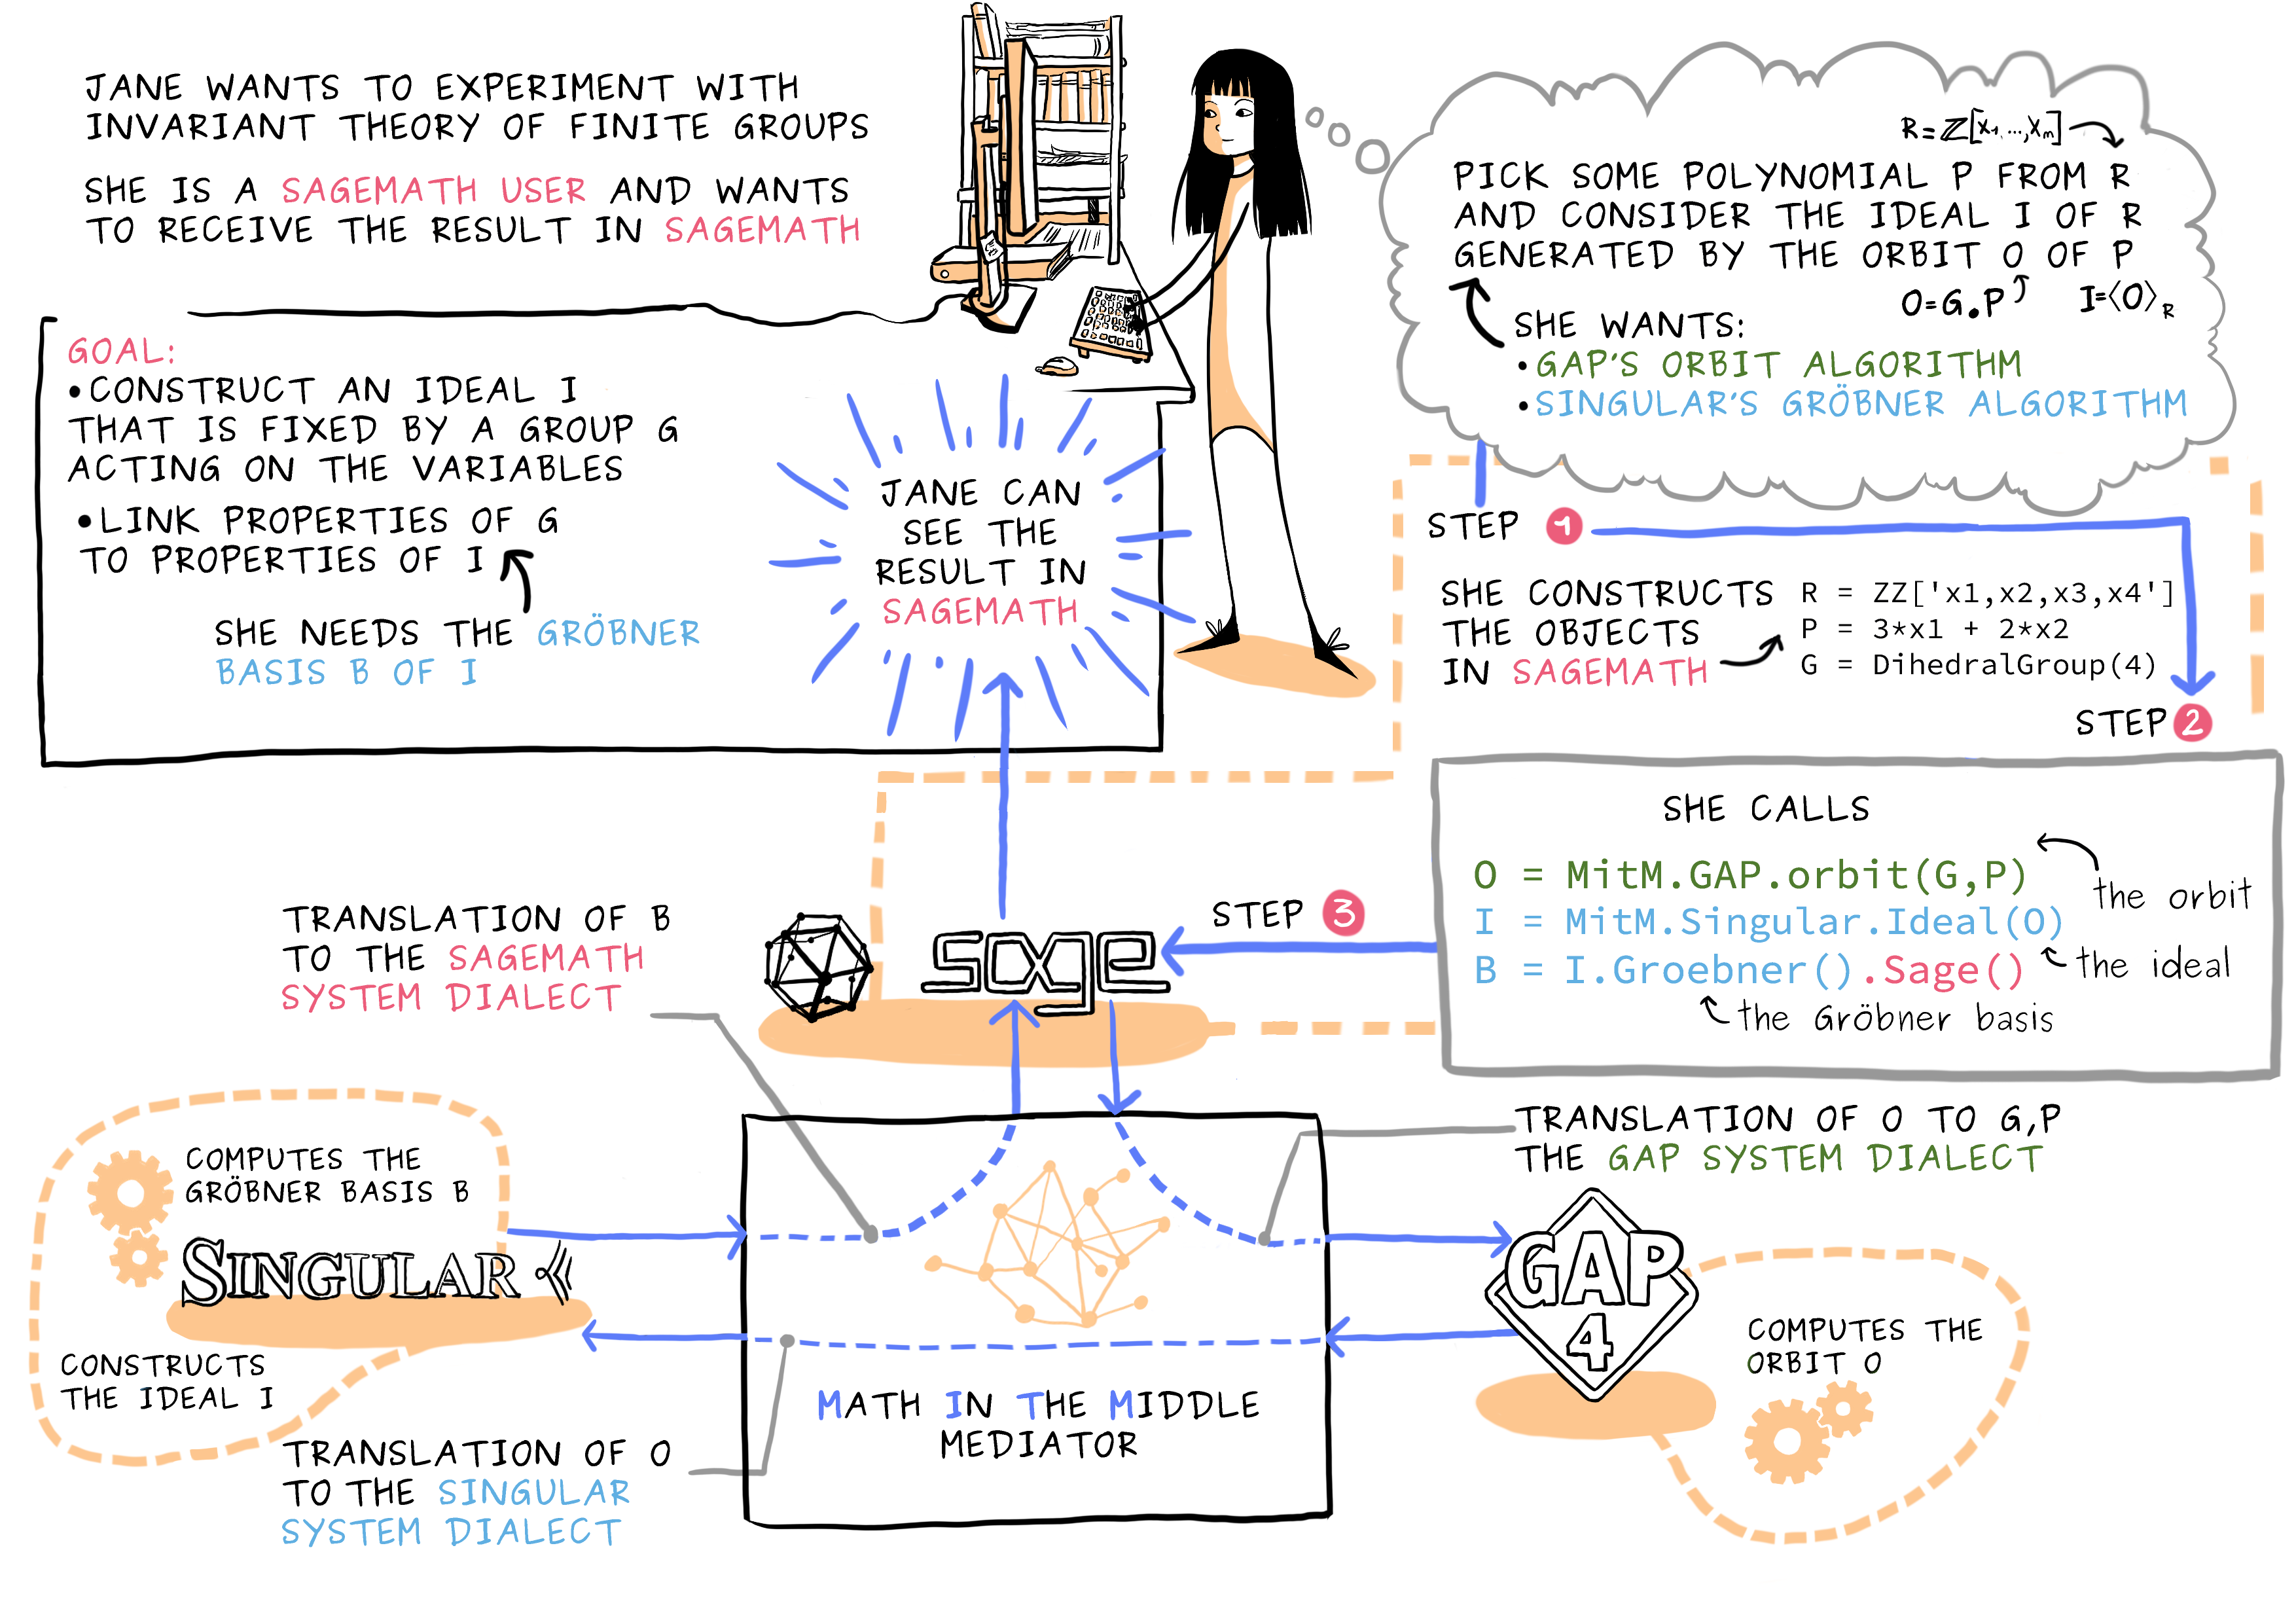
\includegraphics[width=\textwidth]{MitM.png}
\end{frame}

\begin{frame}\frametitle{Integrating BOL and BDL}
\begin{blockitems}{OWL-near option}
\item use BDL to define the primitive types of BOL
\item use those as types of BOL properties
\item Curry-typing throughout
\lec{easy: just merge the grammars}
\end{blockitems}

\begin{blockitems}{SQL-near option}
\item use BDL to define the primitive types of BOL
\item also add ADTs
\item Church typing more prominent
\lec{open question: ADTs in addition to or instead of BOL concepts}
\end{blockitems}

We assume the latter for now without spelling out the details.
\end{frame}

\begin{frame}\frametitle{BDL-Mediated Interoperability}
Idea
 \begin{itemize}
 \item define data types in BDL \glec{or similar typed ontology language}
 \item use ADTs
 \item generate corresponding
  \begin{itemize}
  \item class definitions for programming languages PL
   \lec{one class per ADT}
  \item table definitions in SQL
   \lec{one table per ADT}
  \end{itemize}
 \item use codecs to convert automatically when interchanging data between PL and SQL
 \end{itemize}

Open research problem
 \lec{no shiny solution yet that can be presented in lectures}
\end{frame}

\begin{frame}\frametitle{Codecs in ADT Definitions}
\begin{blockitems}{SQL table schema = list of fields where field is}
\item name
\item type \glec{only types of database supported}
\end{blockitems}

\begin{blockitems}{BDL semantic table schema = list of fields where field is}
\item name
\item type $T$ of \emph{type system} \glec{independent of database}
\item codec for $T$ using primitive objects of database as codes
\glec{see research paper \url{https://kwarc.info/people/frabe/Research/WKR_virtual_17.pdf}}
\end{blockitems}

Codec could be chosen automatically, but we want to allow multiple users a choice of codecs for the same type.
\end{frame}

\begin{frame}[fragile]\frametitle{Example}
Ontology based on BDL-ADTs with additional codec information:
\begin{lstlisting}[basicstyle=\footnotesize]
schema Instructor
  name:    string      codec StandardString
  age:     int         codec StandardInt
  courses: list Course codec CommaSeparatedList CourseAsName
schema Course
  name:     string     codec StandardString
  credits:  float      codec StandardFloat
  semester: Semester   codec SemesterAsString
\end{lstlisting}
\medskip

Generated SQL tables:
\begin{lstlisting}[basicstyle=\footnotesize]
CREATE TABLE Instructor
  (name string, age int, courses string)
CREATE TABLE Course
  (name string, credits float, semester string)
\end{lstlisting}
\end{frame}

\begin{frame}\frametitle{Open Problem: Non-Compositionality}
\begin{blockitems}{Sometimes optimal translation is non-compositional}
\item example translate $list$-type in ADT to comma-separated string in DB
\item better break up $list\,B$ fields in type $A$ into separate table with columns for $A$ and $B$
\end{blockitems}

Similar problems
\begin{itemize}
\item a pair type in an ADT could be translated to two separate columns
\item an option type in an ADT could translated to a normal column using SQL's NULL value
\end{itemize}
\end{frame}

\begin{frame}\frametitle{Open Problem: Querying}
\begin{itemize}
\item General setup
 \begin{itemize}
 \item write SQL-style queries using at the BDL level
 \item automatically encode values when writing to database from PL
 \item automatically decode query results when reading from DB
 \end{itemize}
\item But queries using semantic operations cannot always be translated to DB
 \begin{itemize}
  \item operation $IsSummer: Semester \to bool$ in BDL
  \item query \lstinline|SELECT * FROM course WHERE $IsSummer$(semester)|
  \item how to map $IsSummer$ to SQL?
 \end{itemize}
\item Ontology operations need commuting operations on codes
\begin{itemize}
\item given $f: A\to B$ in BDL, codecs $C,D$ for $A$ and $B$
\item SQL function $f'$ commutes with $f$ iff \\
  \[B.decode (f'(C.encode\,a)) = f(a)\]
  for all $a:A$
\end{itemize}
\end{itemize}
\end{frame}

%\begin{frame}\frametitle{Exercise 5, part 1}
%We build on the implementation of BDL and codecs from Exercise 4 and on the database schemas from Exercise 3.
%
%\begin{enumerate}
% \item Extend the implementation to BDL+ADT (see Slide 101).
% \item Extend 
%  \begin{itemize}
%  \item codecs and codec operators with identifiers $I\bbc (strings)$
%  \item ADT fields with codec expressions $c::=I \bnfalt I(c_1\ldots,c_n)$
%  \end{itemize}
%  and write a function that maps $c$ to the corresponding codec.
%\end{enumerate}
%\end{frame}
%
%\begin{frame}\frametitle{Exercise 5, part 2}
%
%\begin{enumerate}
%\setcounter{enumi}{2}
% \item Write a function that takes a vocabulary (= a list of ADT definitions with codec expressions) and generates an SQL schema for it.
% Use the type returned by the codec as the database type.
% \item Write a function that takes an element $d$ of an ADT and generates the SQL (or CSV) representation of $d$ with all field values encoded by the corresponding codec.
% \item Write a function that takes an ADT name and a SQL or CSV object and applies decoding to build the corresponding ADT element.
% \item Test this by
% \begin{itemize}
% \item writing some of your univis table schemas as ADTs and some example values as ADT elements,
% \item exchanging these with a database and/or via CSV with fellow students' implementations.
% \end{itemize}
%\end{enumerate}
%\end{frame}


%%%%%%%%%%%%%%%%%%%%%%%%%%%%%%%%%%%%%%%%%%%%%%%%%%%%%%%%%%%%%%%%%%%%%%%%%%%%%%%%%%%%%%%%%%
\part{Querying}
\section{Overview}

\begin{frame}\frametitle{General Ideas}
\begin{itemize}
\item Recall
 \begin{itemize}
 \item syntax = context-free grammar
 \item semantics = translation to another language
 \end{itemize}
\item Example: BOL translated to SQL, SFOL, Scala, English
\item Querying = use semantics to answer questions about syntax
\end{itemize}
\medskip

Note:
\begin{itemize}
\item Not the standard definition of querying
\item Design of a new Tetrapod-level notion of querying
 \glec{ongoing research}
\item Subsumes concepts of different names from the various aspects
\end{itemize}
\end{frame}

\begin{frame}\frametitle{Propositions}
syntax with propositions = \\
designated non-terminals for propositions
\medskip

Examples:
\begin{center}
\footnotesize
\begin{tabular}{l|l}
aspect & basic propositions\\
\hline
ontology language & assertions, concept equality/subsumption\\
programming language & equality for some types\\
database language & equality for base types \\
logic & equality for all types\\
natural language & sentences \\
\end{tabular}
\end{center}

Aspects vary critically in how propositions can be formed
\begin{itemize}
\item any program in computation
\item quantifiers in deductions \glec{undecidable}
\item $IN$ in databases
\end{itemize}
\end{frame}

\begin{frame}\frametitle{Propositions as Queries}
Propositions allow defining queries

\begin{center}
\footnotesize
\begin{tabular}{l|ll}
& Query & Result\\
\hline
deduction & proposition & yes/no \\
concretization & proposition with free variables & true ground instances \\
computation & term & value \\
narration & question & answer \\
\end{tabular}
\end{center}
\end{frame}

\begin{frame}\frametitle{Semantics of Propositions}
syntax with propositions = \\
designated non-terminals for propositions \\
\lec{needed to ask queries}
semantics with theorems = \\
designates some propositions as theorems or contradictions
\lec{needed to answer queries}

Note:
\begin{itemize}
\item A propositions may be neither theorem nor contradiction.
\item We say that language has negation if:\\ $F$ theorem iff $\neg F$ contradiction and vice versa.
\end{itemize}

We write $\vdash F$ if $F$ is theorem.
\end{frame}

\section{Deductive Queries}

\begin{frame}\frametitle{Definition}
We assume
\begin{itemize}
\item a semantics $\sem{-}$ from $l$ to $L$
\item $l$ has propositions
\item there is an operation $\truelift$ that maps translations of $l$-propositions to $L$-propositions
 \lec{called truth lifting}
\item $L$ has semantics with propositions
\end{itemize}

We define
\begin{itemize}
\item a deductive query is an $l$-proposition $p$
\item the result is
 \begin{itemize}
 \item yes if $\truelift \sem{p}$ is a theorem of $L$
 \item no if $\truelift \sem{p}$ is a contradiction in $L$
 \end{itemize}
\end{itemize}
\end{frame}

\begin{frame}\frametitle{The Truth-Lift operator}
\begin{blockitems}{Problem with type-preserving translation $\sem{-}$}
\item must translate $F:\prop^l$ to $\sem{F}:\sem{\prop^l}$
\item but need not satisfy $\sem{\prop^l}=\prop^L$ \\
  \glec{$l$-propositions maybe not translated to $L$-propositions}
\item If not, $\vdash^L \sem{F}$ cannot be used to answer query $\vdash^l F$
\end{blockitems}

\begin{blockitems}{Solution: $L$-operator $\truelift: \sem{\prop^l}\to \prop^L$}
\item maps translations of $l$-propositions to $L$-propositions
\item then use $\vdash^L \truelift \sem{F}$ to answer $\vdash^l F$
\end{blockitems}

\begin{blockitems}{Example: probabilistic semantics with cutoff}
\item $\prop^l$: propositions; $\prop^L$: truth values
\item probabilistic semantics: $\sem{\prop^l}=[0;1]$
\item $\truelift$ maps $p\in [0;1]$ to truth value, e.g., via cutoff: $\truelift p = p\geq 0.75$
\end{blockitems}
\end{frame}
  
\begin{frame}\frametitle{Situational Semantics as Translation}
\begin{blockitems}{Example: standard semantics of SFOL in set theory}
\item set theory propositions: truth values $\{0,1\}$
\item situations (= models): provide interpretations for all vocabulary symbols \\
\item semantics is model-specific interpretation function: given vocabulary $V$, $V$-model $M$, and $V$-expression $E$, write $\sem{E}_M$ for semantics of $E$ in $M$
\end{blockitems}

\begin{blockitems}{Reformulate as semantics by translation}
\item vocabulary $V$ translated to set-theoretical vocabulary containing required components of model
\item expression $E$ translated to mapping $\sem{E}:M\mapsto \sem{E}_M$
\end{blockitems}

\begin{blockitems}{Truth-Lift operator defines theorems}
\item $\sem{\prop^l}$ is set of mappings $\mu$ from models to truth values
 \glec{standard notation for $\sem{F}(M)=1$: $\sem{F}_M=1$ or $M\models F$}
\item $\truelift \mu=1$ iff $\mu(M)=1$ for all models $M$ (theorem = true in all models)
\end{blockitems}
\end{frame}

\begin{frame}{Breakout question}
What can go wrong?
\end{frame}

\begin{frame}\frametitle{Problem: Inconsistency}
In general, (in)consistency of semantics
\begin{itemize}
\item Some propositions may be both a theorem and a contradiction.
\item In that case, queries do not have a result.
\end{itemize}

In practice, however:
\begin{itemize}
\item If this holds for some propositions, it typically holds for all of them.
\item In that, we call $L$ inconsistent.
\item We usually assume $L$ to be consistent.
\end{itemize}
\end{frame}


\begin{frame}\frametitle{Problem: Incompleteness}
In general, (in)completeness of semantics
\begin{itemize}
\item We cannot in general assume that every proposition in $L$ is either a theorem or a contradiction.
\item In fact, most propositions are neither.
\item So, queries do not necessarily have a result.
\item We speak of incompleteness. \glec{Note: not the same as the usual (in)completeness of logic}
\end{itemize}

In practice, however:
\begin{itemize}
\item It may be that $L$ is complete for all propositions in the image of $\truelift\sem{-}$.
\item This is the case if $l$ is simple enough \glec{typical for ontology languages}
\end{itemize}
\end{frame}

\begin{frame}\frametitle{Problem: Undecidability}
In general, (un)decidability of semantics:
\begin{itemize}
\item We cannot in general assume that it is decidable whether a proposition in $L$ is a theorem or a contradiction.
\item In fact, it usually isn't.
\item So, we cannot necessarily compute the result of a query.
\item However: If we have completeness, decidability is likely.
 \glec{run provers for $F$ and $\neg F$ in parallel}
\end{itemize}

In practice, however:
\begin{itemize}
\item It may be that $L$ is decidable for all propositions in the image of $\truelift\sem{-}$.
\item This is the case if $l$ is simple enough \glec{typical for ontology languages}
\end{itemize}
\end{frame}

\begin{frame}\frametitle{Problem: Inefficiency}
In general, (in)efficiency of semantics:
\begin{itemize}
\item Answering deductive queries is very slow.
\item Even if we are complete and decidable.
\end{itemize}

In practice, however:
\begin{itemize}
\item Decision procedures for the image of $\truelift\sem{-}$ may be quite efficient.
\item Dedicated implementations for specific fragments.
\item This is the case if $l$ is simple enough \glec{typical for ontology languages}
\end{itemize}
\end{frame}

\section{Contexts and Free Variables}

\begin{frame}\frametitle{Concepts}
Recall the analogy between grammars and typing:

\begin{center}
\begin{tabular}{l|l}
grammars & typing \\
\hline
non-terminal & type \\
production & constructor \\
non-terminal on left of production & return type of constructor \\
non-terminals on right of production & arguments types of constructor \\
terminals on right of production & notation of constructor\\
words derived from non-terminal $N$ & expressions of type $N$
\end{tabular}
\end{center}

We will now add contexts and substitutions.
\end{frame}

\begin{frame}\frametitle{Contexts}
Independent of whether $l$ already has contexts/variables, we can define:
\begin{itemize}
 \item A \emph{context} $\Gamma$ is of the form $x_1:N_1,\ldots,x_n:N_n$ where the
  \begin{itemize}
   \item $x_i$ are names
   \item $N_i$ are non-terminals
  \end{itemize}
  We write this as $\vdash_l \Gamma$.
 \item A \emph{substitution} for $\Gamma$ is of the form $x_1:=w_1,\ldots,x_n:=w_n$ where the
  \begin{itemize}
   \item $x_i$ are as in $\Gamma$
   \item $w_i$ derived from the corresponding $N_i$
  \end{itemize}
  We write this as $\vdash_l \gamma:\Gamma$.
 \item An \emph{expression in context} $\Gamma$ of type $N$ is a word $w$ derived from $N$ using additionally the productions $N_i::= x_i$.\\
 We write this as $\Gamma\vdash_l w:N$.
 \item Given $\Gamma\vdash w:N$ and $\vdash \gamma:\Gamma$ as above, the \emph{substitution of} $\gamma$ in $w$ is obtained by replacing every $x_i$ in $w$ with $w_i$.
 We write this as $w[\gamma]$.
\end{itemize}
\end{frame}


\begin{frame}\frametitle{Contexts under Compositional Translation}
Consider a compositional semantics $\sem{-}$ from $l$ to $L$ between context-free languages.

\begin{itemize}
 \item Every $\vdash_l w:N$ is translated to some $\vdash_L \sem{w}:N'$ for some $N'$.
 \item Compositionality ensures that $N'$ is the same for all $w$ derived from $N$.
 \item We write $\sem{N}$ for that $N'$.
 \item Then we have 
  \[\vdash_l w:N \tb\mimplies\tb \vdash_L \sem{w}:\sem{N}\]
\end{itemize}

Now we translate contexts, substitutions, and variables as well:
\[\sem{x_1:N_1,\ldots,x_n:N_n}:=x_1:\sem{N_1},\ldots,x_n:\sem{N_n}\]
\[\sem{x_1:=w_1,\ldots,x_n:=w_n}:=x_1:=\sem{w_1},\ldots,x_n:=\sem{w_n}\]
\[\sem{x}:=x\]

Then we have
  \[\Gamma\vdash_l w:N \tb\mimplies\tb \sem{\Gamma}\vdash_L \sem{w}:\sem{N}\]
\end{frame}

\begin{frame}\frametitle{Substitution under Compositional Translation}
From previous slide:
\[\sem{x_1:N_1,\ldots,x_n:N_n}:=x_1:\sem{N_1},\ldots,x_n:\sem{N_n}\]
\[\sem{x_1:=w_1,\ldots,x_n:=w_n}:=x_1:=\sem{w_1},\ldots,x_n:=\sem{w_n}\]
\[\sem{x}:=x\]
\[\Gamma\vdash_l w:N \tb\mimplies\tb \sem{\Gamma}\vdash_L \sem{w}:\sem{N}\]

We can now restate the substitution theorem as follows:
  \[\sem{E[\gamma]}=\sem{E}[\sem{\gamma}]\]
\end{frame}

\section{Concretized Queries}

\begin{frame}\frametitle{Definition}
We assume
\begin{itemize}
\item as for deductive queries
\item semantics must be compositional
\end{itemize}

We define
\begin{itemize}
\item a concretized query is an $l$-proposition $p$ in context $\Gamma$
\item a \emph{single} result is a
 \begin{itemize}
 \item a substitution $\vdash_l \gamma:\Gamma$
 \item such that $\vdash_L \truelift \sem{p[\gamma]}$
 \end{itemize}
\item the \emph{result set} is the set of all results
\end{itemize}
\end{frame}

\begin{frame}\frametitle{Example}
\begin{enumerate}
\item BOL ontology:
\[\mathll{concept\, male,\; concept\, person,\;axiom\, male \sqsubseteq person, \\
  individual\, FlorianRabe,\;assertion\, FlorianRabe\, isa\, male}\]
\item Query $x:individual\vdash_{BOL}x \text{ isa } person$
\item Translation to SFOL: $x:\iota\vdash_{SFOL} person(x)$
\item SFOL calculus yields theorem $\vdash_{SFOL}person(FlorianRabe)$
\item Query result $\sem{\gamma}= x:= FlorianRabe$
\item Back-translating the result to BOL: $\gamma= x:= FlorianRabe$
 \glec{back translation is deceptively simple:}
 \glec{translates SFOL-constant to BOL-individual of same name}
\end{enumerate}
\end{frame}

\begin{frame}{Breakout question}
What can go wrong?
\end{frame}

\begin{frame}\frametitle{Problem: Open World}
In general, semantics uses open world:
\begin{itemize}
\item open world: result contains \emph{all known} results
 \lec{same query might yield more results later}
\item closed world: result set contains \emph{all} results
\end{itemize}
 \glec{always relative to concrete database for $L$}

In practice, however,
\begin{itemize}
\item system explicitly assumes closed world
 \glec{typical for databases}
\item users aware of open world and able to process results correctly
\end{itemize}
\end{frame}

\begin{frame}\frametitle{Problem: Infinity of Results}
In general, there may be infinitely many results:
\begin{itemize}
\item e.g., query for all $x$ such that $\vdash x$,
\end{itemize}

In practice, however,
\begin{itemize}
\item systems pull results from finite database \lec{e.g., SQL, SPARQL}
\item systems enumerate results, require user to explicitly ask for more \lec{e.g., Prolog}
\end{itemize}
\end{frame}

\begin{frame}\frametitle{Problem: Back-Translation of Results}
In general, $\sem{-}$ may be non-trivial to invert
\begin{itemize}
\item easy to obtain $\sem{p}$ in context $\sem{\Gamma}$
  \glec{just apply semantics}
\item possible to find substitutions
\[\vdash_L \delta:\sem{\Gamma} \tb\mwhere\tb \sem{\Gamma}\vdash_L \truelift \sem{p}[\delta]\]
  \glec{easiest case: just look them up in database}
\item but how to translate $\delta$ to $l$-substitutions $\gamma$ with
 \[\vdash_l \gamma:\Gamma \tb\mwhere\tb \sem{\Gamma}\vdash_L \truelift \sem{p[\gamma]}\]
 substitution theorem: pick such that $\sem{\gamma}=\delta$
  \glec{the more $\sem{-}$ does, the harder to invert}
\end{itemize}

In practice, however:
\begin{itemize}
\item often only interested in concrete substitutions
\item translation of concrete data usually identity
\end{itemize}
But: practice restricted to what works even if more is needed
\end{frame}


\section{Computational Queries}

\begin{frame}\frametitle{Definition}
We assume
\begin{itemize}
\item the same as for deductive queries
\item semantics has equality/equivalence $\doteq$
\end{itemize}

We define
\begin{itemize}
\item a computational query is an $l$-expression $e$
\item the result is an $l$-expression $e'$ so that $\vdash_L\sem{e}\doteq\sem{e'}$
\end{itemize}
\lec{intuition: $e'$ is the result of evaluating $e$}

If semantics is compositional, $e$ may contain free variables
\lec{evaluate to themselves}
\end{frame}

\begin{frame}\frametitle{Problem: Back-Translation of Results}
In general, $\sem{-}$ may be non-trivial to invert
\begin{itemize}
\item easy to obtain $E:=\sem{e}$
\item possible to find $E'$ with $\vdash_L E'\doteq E$ by working in the semantics
\item non-obvious how to obtain $e'$ such that $\sem{e'}=E'$
\end{itemize}

In practice, however:
\begin{itemize}
\item evaluation meant to simplify, i.e., only useful if $E'$ very simple
\item simple $E'$ usually in the image of $\sem{-}$
\item typical case: $E'$ is concrete data and $e'=E'$ \lec{called a value}
\end{itemize}
\end{frame}

\begin{frame}\frametitle{Problem: Non-Termination}
In general, computation of $E'$ from $E$ might not terminate
\begin{itemize}
 \item while-loops
 \item recursion
 \item $(\lambda x. x\,x)\,(\lambda x. x\,x)$ with $\beta$-rule
 \item simplification rule $x\cdot y \rewrites y\cdot x$ \glec{similar: distributivity, associativity}
\end{itemize}

In practice, however:
\begin{itemize}
\item image of $\sem{-}$ part of terminating fragment
\end{itemize}
But: if $l$ is Turing-complete or undecidable, general termination not possible
\end{frame}

\begin{frame}\frametitle{Problem: Lack of Confluence}
In general, there may be multiple $E'$ that are simpler than $E$
\begin{itemize}
 \item there may be multiple rules that apply to $E$
 \item e.g., $f(g(x))$
  \begin{itemize}
  \item call-by-value: first simplify $g(x)\rewrites y$, then $f(y)\rewrites z$
  \item call-by-name: first plug $g(x)$ into definition of $f$, then simplify
  \end{itemize}
\item Normal vs. canonical form
 \begin{itemize}
 \item normal: $\vdash_L E\doteq E'$
 \item canonical: normal and $\vdash_L E_1\doteq E_2$ iff $E_1'=E_2'$
  \glec{equivalent expressions have identical evaluation}
  \glec{allows deciding equality}
 \end{itemize}
\end{itemize}

In practice, however:
\begin{itemize}
\item image of $\sem{-}$ part of confluent fragment
\item typical: evaluation to a value is canonical form
 \glec{works for BDL-types but not for, e.g., function types}
\end{itemize}
\end{frame}

\section{Narrative Queries}

\begin{frame}\frametitle{Definition}
We assume
\begin{itemize}
\item semantics into natural language
\end{itemize}

We define
\begin{itemize}
\item a narrative query is an $L$-question about some $l$-expressions
\item the result is the answer to the question
\end{itemize}
\end{frame}

\begin{frame}\frametitle{Problem: Unimplementable}
very expressive = very difficult to implement
\begin{itemize}
\item Natural language understanding
 \begin{itemize}
 \item no implementable syntax of natural language
  \glec{needs restriction to controlled natural language}
 \item specifying semantics hard even when controlled
 \end{itemize}
\item Knowledge base for question answering needed
 \begin{itemize}
 \item very large \glec{must include all common sense}
 \item might be inconsistent \glec{common sense often is}
 \item finding answers still very hard
 \end{itemize}
\end{itemize}
 
In practice, however:
\begin{itemize}
 \item accept unreliability \glec{attach probability measures to answers}
 \item implement special cases \glec{e.g., lookup in databases like Wikidata}
 \item search knowledge base for related statements \glec{Google, Watson}
\end{itemize}
\end{frame}


\section{Syntactic Querying}

\begin{frame}\frametitle{Search}
\begin{itemize}
\item ``search'' not systematically separated from ``querying''
\item often interchangeable
\item querying tends to imply formal languages for queries with well-specified semantics
 \lec{e.g., SQL}
\item search tends to imply less targeted process
 \lec{e.g., Google}
\end{itemize}
\lec{we will not distinguish between the two}
\end{frame}

\begin{frame}\frametitle{Syntactic vs. Semantic Querying}
\begin{blockitems}{Semantic querying}
\item Query results specified by vocabulary $V$ but (usually) not contained in it
\item Query answered using semantics of language
\item Challenge: apply semantics to find results
 \begin{itemize}
 \item deductive query $\vdash f:\prop$ requires theorem prover 
 \item computation query $\vdash e:E$ requires evaluator
 \item concrete query $\Gamma\vdash f:\prop$ requires enumerating all substitutions, running theorem prover/evaluator on all of them
 \end{itemize}
\end{blockitems}
\lec{what we've looked at so far}

\begin{blockitems}{Syntactic querying}
\item Query is an expression $e$
\item Result is set of occurrences of $e$ in $V$
\item Independent of semantics
\item Much easier to realize
\end{blockitems}
\end{frame}

\begin{frame}\frametitle{Challenges for Syntactic Search}
Easier to realize $\to$ scale until new challenges arise
\begin{itemize}
\item large vocabularies
 \begin{itemize}
 \item narrative: all text documents in a domain \glec{e.g., all websites, all math papers}
 \item deductive: large repositories of formalization in proof assistants
  \glec{$10^5$ theorems}
 \item computational: package managers for all programming languages
 \item concrete: all databases in a domain \glec{TBs routine}
 \end{itemize}
\item incremental indexing: reindex only new/changed parts
\item incremental search to handle large result sets \glec{pagination}
\item sophisticated techniques for
 \begin{itemize}
 \item indexing: to allow for fast retrieval
 \item similarity: to select likely results
 \item quality: to rank selected results
\end{itemize}
\item integration of some semantic parts
\end{itemize}
\end{frame}

\begin{frame}\frametitle{Overview}
\begin{itemize}
\item Deduction 
 \begin{itemize}
 \item semantic: theorem proving called search
 \item syntactic: text search
 \end{itemize}
\item Concretization
 \begin{itemize}
 \item semantic: complex query languages (nestable queries)
  \glec{SQL, SPARQL}
 \item syntactic: search by identifier (linked data)
 \end{itemize}
\item Computation
 \begin{itemize}
 \item semantic: interpreters called execution
 \item mixed: IDEs search for occurrences, dependencies
 \item syntactic: search in IDE, package manager
\end{itemize}
\item Narration:
 \begin{itemize}
 \item semantic: very difficult
 \item syntactic: bag of words search
 \end{itemize}
\end{itemize}
\end{frame}


\begin{frame}\frametitle{Abstract Definition: Document}
\textbf{Document} =
\begin{itemize}
\item file or similar resource that contains vocabularies
\item often with comments, metadata
\item different names per aspect
\begin{itemize}
\item deduction: formalization, theory, article
\item computation: source files
\item concretization: database, ontology ABox
\item narrative: document, web site
\end{itemize}
\end{itemize}

\textbf{Library} =
\begin{itemize}
\item collection of documents
\item usually structured into folders, files or similar
\item often grouped by user access \glec{e.g., git repository}
\item vocabularies interrelated within and across libraries
\end{itemize}
\end{frame}

\begin{frame}\frametitle{Abstract Definition: Document Fragment}
\textbf{Fragment} = subdivision of documents into nested semantic units

Examples
\begin{itemize}
\item deductive: theory, section, theorem, definition, proof step, etc.
\item computational: class, function, command, etc.
\item concrete: table, row, cell
\item narrative: section, paragraph, etc.
\end{itemize}

Assign unique \textbf{fragment URI}, e.g., LIB/DOC?FRAG where
\begin{itemize}
\item LIB: base URI of library \lec{e.g., repository URL}
\item DOC: path to document within library \lec{e.g., folder structure, file name}
\item FRAG: id of fragment within document \lec{e.g., class name/method name}
\end{itemize}
\end{frame}

\begin{frame}\frametitle{Abstract Definition: Index(er)}
\textbf{Indexer} consists of
\begin{itemize}
\item data structure $O$ for indexable objects
 \lec{specific to aspect, index design}
 \glec{e.g., words, syntax trees}
\item function that maps library to index \glec{the indexing}
\end{itemize}

\textbf{Index entry} consists of
\begin{itemize}
\item object that occurred in the library
\item URI of the containing fragment
\item information on where in the fragment it was found
\end{itemize}

\textbf{Index} = set of index entries
\end{frame}

\begin{frame}\frametitle{Abstract Definition: Query and Result}
Given
\begin{itemize}
\item indexer $I$ with data structure $O$
\item set of libraries
\item union of their indexes  \lec{computed once, queried often}
\end{itemize}

\textbf{Query} = object $\Gamma \vdash^I q:O$

\textbf{Result} consists of
\begin{itemize}
\item index entry with object $o$
\item substitution for $\Gamma$ such that $q$ matches $o$
 \lec{definition of ``match'' index-specific, e.g., $q[\gamma]=o$}
\end{itemize}

\textbf{Result set} = set of all results in the index
\end{frame}

\begin{frame}\frametitle{Bag of Words Search}
Definition:
\begin{itemize}
\item Index data structure = sequences of words (n-grams) up to a certain length
\item Query = bag of words
 \glec{bag = multiset}
\item Match: (most) words in query occur in same n-gram or n-grams near each other
\end{itemize}

Example implementations
 \begin{itemize}
 \item internet search engines for websites
 \item Elasticsearch: open source engine for custom vocabularies
 \end{itemize}

Mostly used for narrative documents
\begin{itemize}
 \item can treat concrete values as words \glec{e.g., numbers}
 \item could treat other expressions as words \glec{works badly}
\end{itemize}

\end{frame}

\begin{frame}\frametitle{Symbolic Search}
Definition:
\begin{itemize}
\item Index data structure = syntax tree (of any grammar) of expressions $o$ with free/bound variables
\item Query = expression $q$ with free (meta-)variables
\item Match: $q[\gamma]=_\alpha o$, i.e., up to variable renaming
\end{itemize}

Example implementation
 \begin{itemize}
 \item MathWebSearch \lec{see separate slides on MathWebSearch in the repository}
 \end{itemize}

Mostly used for formal documents
\begin{itemize}
 \item deductive
 \item computational
\end{itemize}
\end{frame}

\begin{frame}\frametitle{Knowledge Graph Search}
Definition:
\begin{itemize}
\item Index data structure = assertion forming node/edge in a knowledge graph
\item Index = big knowledge graph $G$
\item Query = knowledge graph $g$ with free variables
\item Match: $g[\gamma]$ is part of $G$
\end{itemize}

Example implementations
 \begin{itemize}
 \item SPARQL engines without consequence closure \glec{i.e., the most common case in practice}
 \item graph databases
 \end{itemize}

Mainly used for ABoxes of untyped ontologies
\end{frame}

\begin{frame}\frametitle{Value Search}
Definition:
\begin{itemize}
\item Index data structure = BDL values $v$
\item Query = BDL expression $q$ with free variables
\item Match: $q[\gamma]=v$
\end{itemize}

Example implementations
 \begin{itemize}
 \item no systematic implementation yet
 \item special cases part of most database systems
 \end{itemize}

Could be used for values occurring in any document
\begin{itemize}
 \item all aspects
 \item may need to decode/encode before putting in index
\end{itemize}
\end{frame}

\begin{frame}\frametitle{Cross-Aspect Occurrences}
Observation
\begin{itemize}
\item libraries are written in one primary aspect
\item indexer focuses on one aspect and kind of object
\item but documents may contain indexable objects of any index
\end{itemize}
\end{frame}

\begin{frame}\frametitle{Cross-Aspect Occurrences: Examples}
\begin{itemize}
\item Any library can contain
\begin{itemize}
 \item metadata on fragments
  \begin{itemize}
  \item relation assertions induce knowledge graph structure between fragments
  \item property assertions contain values narrative, symbolic objects, or values
 \end{itemize}
 \item cross-references to fragments of any other library
 \item narrative comments
\end{itemize}
\item Narrative text may contain symbolic expressions \glec{STEM documents}
\item Database table may have columns containing
 \begin{itemize}
 \item text
 \item encoded BDL values
 \item symbolic expression (often as strings)
 \end{itemize}
\item Symbolic fragments may contain database references
 \glec{e.g., when using database for persistent memoization}
\end{itemize}
\end{frame}

\begin{frame}\frametitle{A New Indexing Design}
recent paper \url{https://kwarc.info/people/frabe/Research/BKR_mdql_20.pdf} \glec{with K. Bercic}

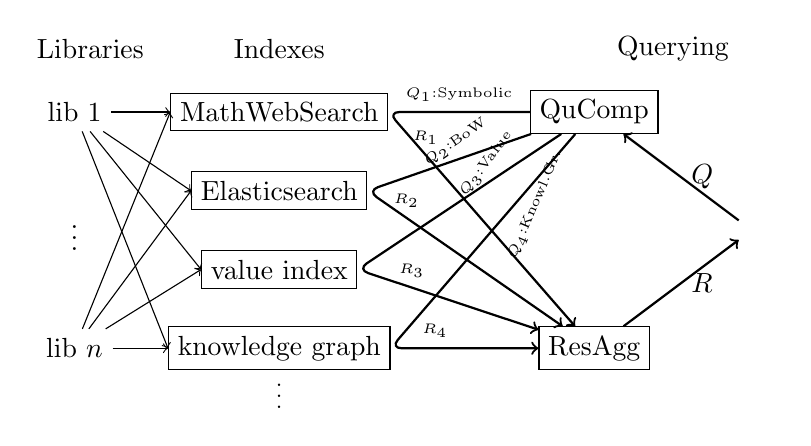
\begin{tikzpicture}[xscale=2]
  \node at (.8,2.8) {Libraries};
  \node (l1) at (0.7,2) {lib 1};
  \node at (.7,.5) {\vdots};
  \node (ln) at (0.7,-1) {lib $n$};
  \node at (2,2.8) {Indexes};
  \node[draw] (si) at (2,2) {MathWebSearch};
  \node[draw] (ni) at (2,1) {Elasticsearch};
  \node[draw] (ci) at (2,0) {value index};
  \node[draw] (oi) at (2,-1) {knowledge graph};
  \node (d) at (2,-1.5]) {\footnotesize\vdots};
  \draw[->] (l1) -- (si);
  \draw[->] (l1) -- (ni.west);
  \draw[->] (l1) -- (oi.west);
  \draw[->] (l1) -- (ci.west);
  \draw[->] (ln) -- (si.west);
  \draw[->] (ln) -- (ni.west);
  \draw[->] (ln) -- (ci.west);
  \draw[->] (ln) -- (oi.west);
  \node at (4.5,2.8) {Querying};
  \node[draw] (qc) at (4,2) {QuComp};
  \node[draw] (qa) at (4,-1) {ResAgg};

  \draw[->,rounded corners,thick] (qc) -- node[above] {\tiny $Q_1$:Symbolic}
                                             (si.east) -- node[pos=.2,above] {\tiny $R_1$} (qa);
  \draw[->,rounded corners,thick] (qc) -- node[pos=.4,above,sloped] {\tiny $Q_2$:BoW}
                                             (ni.east) -- node[pos=.2,above] {\tiny $R_2$} (qa); 
  \draw[->,rounded corners,thick] (qc) -- node[pos=.3,above,sloped] {\tiny $Q_3$:Value}
                                              (ci.east) -- node[pos=.3,above] {\tiny $R_3$} (qa); 
  \draw[->,rounded corners,thick] (qc) -- node[pos=.3,below,sloped] {\tiny $Q_4$:Knowl.Gr.}
                                              (oi.east) -- node[pos=.3,above] {\tiny$R_4$}(qa);

  \node[minimum width=.8cm] (u) at (5,.5) {};

  \draw[->,thick] (u) -- node[right] {$Q$} (qc);
  \draw[->,thick] (qa) -- node[right] {$R$} (u);
\end{tikzpicture}
\end{frame}

\begin{frame}\frametitle{A New Indexing Design (2)}
Tricky question: What is the query language that allows combining queries for each index?
\medskip

Easy:
\begin{itemize}
\item query = conjunction of atomic queries
\item each atom queries one index
\item QuComp splits into atoms
\item ResAgg take intersection of results
\end{itemize}
\medskip

Better: allow variables to be shared across atoms
\lec{open research question}
\end{frame}

\begin{frame}\frametitle{A New Indexing Design: Example}
Consider
\begin{itemize}
\item table of graphs with human-recognizable names and arc-transitivity property\\
indexed into
\begin{itemize}
\item value index for the graph \lec{\texttt{sparse6} codec}
\item Boolean computed property for the arc-transitivity in knowledge graph
\item text index for name
\end{itemize}
\item papers from arXiv in narrative index\\
indexed into
\begin{itemize}
\item narrative index for text
\item MathWebSearch for formulas
\item knowledge graph for metadata
\end{itemize}
\end{itemize}

Query goal: find arc-transitive graphs mentioned by name in articles with h-index greater than 50

%\[\mdql{G:Graph}{\\\cn{arcTransitive}(G), \atomnarr{F}{\cn{Name}(G), \narr{graph}},
% \\\atomorg{F}{\cn{partOf}}{P}, \atomorg{P}{\cn{bibo:publishedIn}}{J}, \atomorg{J}{\cn{spar:hasHindex}}{H}, H > 50}\]
%The first atom in the $\WHERE$-clause returns all arc-transitive graphs $G$ in the concrete index.
%
%The second atom retrieves the names of these graphs and runs a narrative query for them.
%This includes evaluating the expression $\cn{Name}(G)$ into a string by retrieving the corresponding value from the concrete index.
%To avoid false-positives, we include the word $\narr{graph}$ in the narrative atom.
%It instantiates $F$ with the identifier of the matching fragment, presumably a part of a paper.
%
%The next three atoms are organizational atoms that perform a SPARQL query retrieving first the identifier $P$ of the paper containing $F$, the identifiers $J$ of the journal it appeared in, and its h-index $H$.
%$H$ is a concrete value that is reused in the final concrete query on the size of $H$.
%
%Finally, we throw away all variables from the obtained substitutions except for the graphs $G$.
%Alternatively, we could include $P$ in the $\SELECT$-clause to also return the paper.
\end{frame}

\begin{frame}\frametitle{Integrating Semantic Querying}
Word search
\begin{itemize}
\item find multi-meaning words for only one meaning \glec{``normal'' in math}
\item special treatment of certain queries \glec{e.g., ``weather'' in Google}
\end{itemize}

Symbolic search
\begin{itemize}
\item match query $e\doteq e'$ against occurrence $e'\doteq e$
\item similarly: associativity, commutativity, etc.
\item slippery slope to deductive queries
\end{itemize}

Value search
\begin{itemize}
\item match query $1.5$ against interval $1.4\pm 0.2$
\item match query $5\cdot x$ against $25$
\item slippery slope to computational queries
\end{itemize}
\lec{frontiers of research --- in our group: for STEM documents}
\end{frame}



%%%%%%%%%%%%%%%%%%%%%%%%%%%%%%%%%%%%%%%%%%%%%%%%%%%%%%%%%%%%%%%%%%%%%%%%%%%%%%%%%%%%%%%%%%
\part{Semantics}
\section{Kinds of Semantics}

\begin{frame}\frametitle{Recall}
Recall:

\begin{center}
\begin{tabular}{l|l}
Syntax & Data \\
\hline
Semantics & Knowledge
\end{tabular}
\end{center}

Representing
\begin{itemize}
\item syntax = formal language
\begin{itemize}
\item grammar  \glec{context-free part}
\item type system \glec{context-sensitive well-formedness}
\end{itemize}
\item data = words in the syntax
\begin{itemize}
\item set of vocabularies
\item set of typed expressions for each vocabulary
\end{itemize}
\item semantics = \alert{???}
\item knowledge = emergent property of having well-formed words with semantics
\end{itemize}
\end{frame}

\begin{frame}\frametitle{Relative Semantics by Translation}
Components:
\begin{itemize}
\item Two syntaxes
\begin{itemize}
\item object-language $l$ \glec{e.g., BOL}
\item meta-language $L$ \glec{e.g., SFOL, Scala, SQL, English}
\end{itemize}
\item Semantics of $L$ assumed fixed
 \glec{captures what we already know}
\item Semantics of $l$ by translation into $L$
\end{itemize}
\lec{semantics of $l$ \emph{relative} to to existing semantics of $L$}

Problem: just kicking the can?
\end{frame}

\begin{frame}\frametitle{Discussion of Semantics by Translation}
\begin{blockitems}{Advantages}
\item a few meta-languages yield semantics for many languages
\item easy to develop new languages
\item good connection between syntax and semantics via compositionality, substitution theorem
\end{blockitems}

\begin{blockitems}{Disadvantages}
\item does not solve the problem once and for all
\item impractical without implementation of semantics of meta-language
\item meta-languages typically much more expressive than needed for object-languages
\item translations can be difficult, error-prone
\end{blockitems}

Also needed: absolute semantics
\end{frame}

\begin{frame}\frametitle{Absolute vs. Relative Semantics}
Absolute = self-contained, no use of meta-language $L$

\begin{blockitems}{Get off the ground}
 \item semantics for a few important meta-languages
  \glec{e.g., FOL, assembly language, set theory}
 \item relative semantics for all other languages, e.g.,
  \begin{itemize}
  \item model theory: logic $\to$ set theory
  \item compilation: Scala $\to$ JVM $\to$ assembly
  \end{itemize}
\end{blockitems}

\begin{blockitems}{Redundant semantics}
 \item common to give
 \begin{itemize}
  \item relative and absolute semantics for same syntax
  \item multiple relative semantics
   \glec{translations to different aspects}
  \item sometimes even maybe multiple absolute ones
 \end{itemize}
 \item Allows understanding syntax from multiple perspectives
 \item Allows cross-checking \glec{show equivalence of two semantics}
\end{blockitems}
\end{frame}


\begin{frame}\frametitle{Example: Recall Syntax of Arithmetic Language}
Syntax: represented as formal grammar

\begin{commgrammar}
\gcomment{Numbers}\\
\gprod{N}{0\bnfalt 1}{literals}\\
\galtprod{N+N}{sum}\\
\galtprod{N*N}{product}\\
\gcomment{Formulas}\\
\gprod{F}{N\doteq N}{equality}\\
\galtprod{N\leq N}{ordering by size}\\
\end{commgrammar}

Implementation as inductive data type
\end{frame}

\begin{frame}\frametitle{Example: Absolute Semantics}
\begin{blockitems}{Represented as judgments defined by sets of rules}
\item unclear what judgments to use
\item here: computation $\der N \rewrites N$ and truth $\der F$
\end{blockitems}

For numbers $n$: Rules to normalize numbers into values
\[\rul{}{\der N+0\rewrites N} \tb \rul{}{\der N*0\rewrites 0}\tb \rul{}{\der N*1\rewrites N}\]
\[\rul{}{\der N*(R+S)\rewrites N*R+N*S}\]
and their commutative variants as well as
\[\rul{}{\der L+(M+N)\rewrites (L+M)+N}\]


For formulas $f$: rules to determine true formulas
\[\rul{}{\der N\doteq N} \tb \rul{}{\der N\leq N} \tb \rul{\der L\leq M}{\der L+N\leq M+N}\]
\end{frame}

\begin{frame}\frametitle{Example: Absolute Semantics (2)}
Checking if an absolute semantics works as intended is hard.

Here: number rules allow
\begin{enumerate}
\item eliminating all cases where arguments of $*$ are $0$, $1$, or $+$; thus, no more $*$
\item eliminating all cases where arguments of $+$ are $0$
\item shift brackets of nested $+$ to the left
\item left: $0$ or $(\ldots(1+1)\ldots+1)$ --- isomorphic to natural numbers
\end{enumerate}
formula rules allow
\begin{enumerate}
\item concluding equality if identical normal forms
\item reducing $M+1\leq N+1$ to $M\leq N$, repeat until $N\leq N$
\end{enumerate}
\end{frame}


\begin{frame}\frametitle{Example: Relative Semantics}
Semantics: represented as translation into known language
\medskip

Problem: Need to choose a known language first\\
Here: unary numbers represented as strings

Built-in data (strings and booleans):
\begin{commgrammar}
%\gcomment{Strings}\\
\gprod{S}{""}{empty}\\
\galtprod{(\texttt{Unicode)}}{character sequence}\\
%\gcomment{Booleans}\\
\gprod{B}{\cn{true}}{truth}\\
\galtprod{\cn{false}}{falsity}\\
\end{commgrammar}

Built-in operations to work on the data:
\begin{itemize}
\item concatenation of strings $S\bbc \cn{conc}(S,S)$
\item replacing all occurrences of $c$ in $S_1$ with $S_2$ $S\bbc \cn{replace}(S_1,c,S_2)$
\item equality test: $B\bbc S_1==S_2$
\item prefix test: $B\bbc \cn{startsWith}(S_1,S_2)$
\end{itemize}
\end{frame}

\begin{frame}\frametitle{Example: Relative Semantics}
\begin{blockitems}{Represented as function from syntax to semantics}
\item mutually recursive, inductive functions for each non-terminal symbol
\item compositional: recursive call on immediate subterms of argument
\end{blockitems}

For numbers $n$: semantics $\sem{n}$ is a string
\begin{itemize}
\item $\sem{0}=""$
\item $\sem{1}="|"$
\item $\sem{m+n}=\cn{conc}(\sem{m},\sem{n})$
\item $\sem{m*n}=\cn{replace}(\sem{m},"|",\sem{n})$
\end{itemize}
\medskip

For formulas $f$: semantics $\sem{f}$ is a boolean
\begin{itemize}
\item $\sem{m\doteq n}=\sem{m}==\sem{n}$
\item $\sem{m\leq n}=\cn{startsWith}(\sem{n},\sem{m})$
\end{itemize}
\end{frame}

\begin{frame}\frametitle{Example: Equivalence of Semantics}
\begin{blockitems}{For formulas}
\item if $\der F$, then $\sem{F}=true$ 
 \glec{usually called \emph{soundness}}
\item if $\sem{F}=true$, then $\der F$
 \glec{usually called \emph{completeness}}
\end{blockitems}

\begin{blockitems}{For numbers}
\item $\der N\rewrites 0$ iff $\sem{N}=""$
\item $\der N\rewrites (\ldots(1+1)\ldots+1)$ iff $\sem{N}="|\ldots|"$
\end{blockitems}
\end{frame}

\begin{frame}\frametitle{No Perfect Model for Absolute Semantics}
\begin{itemize}
\item Machine-actionable requires reduction to finite set of rules
 \lec{whatever a rule is}
\item Does not work for most domains
 \begin{itemize}
 \item practical argument: any practically interesting system has too many rules
  \glec{cf. physics, e.g., three-body problem already chaotic}
 \item theoretical argument: no language can fully model itself
  \glec{cf. G\"odel's incompleteness theorems}
 \end{itemize}
\item Imperfect representation of intended semantics required
\lec{focus on some \emph{aspect}}
\end{itemize}

Big question: what aspects to focus on?
\end{frame}

\begin{frame}\frametitle{Querying as a Guide}
\begin{blockitems}{Idea}
\item Very difficult to choose aspects for absolute semantics
\item Turn problem around
 \begin{itemize}
 \item ask what the practical purpose of the semantics could be
 \item then choose aspects that allow realizing that purpose
 \end{itemize}
\end{blockitems}

Meta-remark: We do relative semantics first even though absolute semantics conceptually comes first.

\begin{blockitems}{Querying as the Purpose}
\item Before: identified different kinds of querying
 \lec{focussing on different aspects of knowledge}
\item Now: each induces a kind of absolute semantics
\end{blockitems}
\end{frame}


\section{Relative Semantics for BOL}

\begin{frame}\frametitle{Semantics of BOL}
\begin{center}
\begin{tabular}{lll}
Aspect & kind of semantic language & semantic language\\
\hline 
deduction & logic & SFOL \\
concretization & database language & SQL \\
computation & programming language & Scala \\
narration & natural language & English \\
\end{tabular}
\end{center}
\end{frame}

\begin{frame}\frametitle{Deductive Semantics of BOL in SFOL}
We discuss
\begin{itemize}
\item the grammar of SFOL
\item context-sensitive languages with variable binding (of which SFOL is an example)
\item an implementation of SFOL in Scala
\item the translation from BOL to SFOL
\item compositionality of the translation
\item the issue of
 \begin{itemize}
 \item non-compositionality
 \item the need for a semantic prefix
 \end{itemize}
\end{itemize}
see details in the lecture notes
\end{frame}


\begin{frame}\frametitle{General Definition}
A semantics by translation consists of
\begin{itemize}
 \item syntax: a formal system $l$
 \item semantic language: a formal system $L$
  \glec{different or same aspect as $l$}
 \item semantic prefix: a vocabulary $P$ in $L$
  \glec{formalizes fundamentals that are needed to represent $l$-objects}
 \item interpretation: translates every $l$-vocabulary $T$ to an $L$-vocabulary $P,\sem{T}$
\end{itemize}
\end{frame}

\begin{frame}\frametitle{Common Principles}
Properties shared by all semantics by translation
\lec{not part of formal definition, but best practices}
\begin{itemize}
 \item $l$-declaration translated to $L$-declaration for the same name
 \item vocabularies translated declaration-wise
 \item one inductive function for every kind of complex $l$-expression
  \begin{itemize}
   \item individuals, concepts, relations, properties, formulas
   \item maps $l$-expressions to $L$-expressions
  \end{itemize}
 \item atomic cases (base cases): $l$-identifier translated to $L$-identifier of the same name
  \glec{or something very similar}
 \item complex cases (step cases): compositional
\end{itemize}
\end{frame}

\begin{frame}\frametitle{Translation vs. Embedding}
\begin{blockitems}{Translation}
\item as above, $l$ and $L$ are at the same level
\item $l$-declarations represented as $L$-declarations
\glec{also called shallow embedding}
\end{blockitems}

\begin{blockitems}{Embedding}
\item $L$ is used as meta-language to represent $l$
 \glec{e.g., $L$ is programming language to implement $l$}
\item $l$-declarations represented as $L$-objects using an inductive type
\glec{also called deep embedding}
\end{blockitems}
\end{frame}

\begin{frame}\frametitle{Compositionality}
Case for operator $*$ in translation function compositional iff \\
interpretation of $*(e_1,\ldots,e_n)$ only depends on on the interpretation of the $e_i$

\[\sem{*(e_1,\ldots,e_n)}=\sem{*}(\sem{e_1},\ldots,\sem{e_n})\]
for some function $\sem{*}$
\bigskip

Example: $;$-operator of BOL in translation to FOL
\begin{itemize}
 \item translation: $\sem{R_1 ; R_2}= \exists m:\iota.\sem{R_1}(x,m)\wedge \sem{R_2}(m,y)$
 \item special case of the above via
  \begin{itemize}
  \item $*=;$
  \item $n=2$
  \item $\sem{;}=(p_1,p_2)\mapsto \exists m:\iota.p_1(x,m)\wedge p_2(m,y)$
  \end{itemize}
 \item Indeed, we have $\sem{R_1;R_2}=\sem{;}(\sem{R_1},\sem{R_2})$
\end{itemize}
\end{frame}


\begin{frame}\frametitle{Compositionality (2)}
Translation compositional iff
\begin{itemize}
\item one translation function for each non-terminal
 \glec{all written $\sem{-}$}
\item each defined by one induction on syntax
 \glec{i.e., one case for production}
 \glec{mutually recursive}
\item all cases compositional
\end{itemize}
\bigskip

Substitution theorem: a compositional translation satisfies
\[\sem{E(e_1,\ldots,e_n)}=\sem{E}(\sem{e_1},\ldots,\sem{e_n})\]
for
\begin{itemize}
\item every expression $E(N_1,\ldots,N_n)$ with non-terminals $N_i$
\item some function $\sem{E}$ that only depends on $E$
\end{itemize}
\end{frame}


\begin{frame}\frametitle{Compositionality (3)}
\[\sem{E(e_1,\ldots,e_n)}=\sem{E}(\sem{e_1},\ldots,\sem{e_n})\]
for every expression $E(N_1,\ldots,N_n)$ with non-terminals $N_i$
\bigskip

Now think of
\begin{itemize}
\item variable $x_i$ of type $N_i$ instead of non-terminal $N_i$
\item $E(x_1,\ldots,x_n)$ as expression with free variables $x_i$ of type $N_i$
\item expressions $e$ derived from $N$ as expressions of type $N$
\item $E(e_1,\ldots,e_n)$ as result of substituting $e_i$ for $x_i$
\item $\sem{E}(x_1,\ldots,x_n)$ as (semantic) expression with free variables $x_i$
\end{itemize}

Then both sides of equations act on $E(x_1,\ldots,x_n)$:
\begin{itemize}
\item left side yields $\sem{E(e_1,\ldots,e_n)}$ by
\begin{itemize}
\item first substitution $e_i$ for $x_i$
\item then semantics $\sem{-}$ of the whole
\end{itemize}
\item right side yields $\sem{E}(\sem{e_1},\ldots,\sem{e_n})$ by
\begin{itemize}
\item first semantics $\sem{-}$ of all parts
\item then substitution $\sem{e_i}$ for $x_i$
\end{itemize}
\end{itemize}
\lec{semantics commutes with substitution}
\end{frame}

\begin{frame}\frametitle{Non-Compositionality}
\begin{blockitems}{Examples}
 \item deduction: cut elimination, translation from natural deduction to Hilbert calculus
 \item computation: optimizing compiler, e.g., loop unrolling
 \item concretization: query optimization, e.g., turning a WHERE of a join into a join of WHEREs,
 \item narration: ambiguous words are translated based on context
\end{blockitems}

\begin{blockitems}{Typical sources}
 \item subcases in a case of translation function
  \begin{itemize}
  \item based on inspecting the arguments, e.g., subinduction
  \item based on context
  \end{itemize}
 \item custom-built semantic prefix
\end{blockitems}
\end{frame}

\section{Absolute Semantics for BOL}

\begin{frame}\frametitle{Judgments}
Typing:  \[\Gamma\vdash^{BOL}_V e:E\]
Deduction: \[\Gamma\vdash^{BOL}_V F\]

Propositions $\prop$:
\begin{itemize}
\item $C\sqsubseteq D$, $C\Equiv D$
\item all three kinds of assertions
\end{itemize}

Notation:
\begin{itemize}
\item We drop the superscript $^{BOL}$ everywhere.
\item We drop the subscript $_V$ unless we need to use $V$.
\item We drop the context $\Gamma$ unless we need to use/change $\Gamma$.
\end{itemize}
\end{frame}

\begin{frame}\frametitle{Typing}
Trivial intrinsic typing (Church) $\vdash e:^{int} E$
\begin{itemize}
\item $E$ is a non-terminal
\item $e$ an expression derived from $E$
\end{itemize}
\medskip

Refined by extrinsic typing (Curry) $\vdash e :^{ext} E$
\begin{itemize}
\item $e$ is an individual, i.e., $\vdash e :^{int} I$
\item $E$ is a concept, i.e., $\vdash E :^{int} C$
 \glec{where $I$ and $C$ are the non-terminals from the grammar}
\item $e$ has concept $E$, i.e., $\vdash e \isa E$
\end{itemize}
\end{frame}

\begin{frame}\frametitle{Propositions as Types}
Say also $\vdash p:f$ for proofs $p$ of proposition $f$
\lec{in particular: $x:f$ in contexts to make local assumptions}
\medskip

Notation:
\[\Gamma,\; f \tb\text{instead of} \tb \Gamma,\;p:f\]
\glec{sufficient if we only state the rules, not build proofs}
\end{frame}

\begin{frame}\frametitle{Lookup Rules}
The main rules that need to access the vocabulary:
\[\rul{f\minn V}{\vdash_V f}\]
\glec{for assertions or axioms f}
\medskip

Assumptions in the context are looked up accordingly:
\[\rul{x:f\minn \Gamma}{\Gamma\vdash f}\]
\end{frame}

\begin{frame}\frametitle{Rules for Subsumption and Equality}
Subsumption is an order with respect to equality:
\[\rul{}{\vdash c\sqsubseteq c}\]

\[\rul{\vdash c\sqsubseteq d \tb \vdash d\sqsubseteq e}{\vdash c\sqsubseteq e}\]

\[\rul{\vdash c\sqsubseteq d \tb \vdash d\sqsubseteq c}{\vdash c\Equiv d}\]

Equal concepts can be substituted for each other:
\[\rul{\vdash c\Equiv d\tb x:C\vdash f(x):\prop \tb \vdash f(c)}{\vdash f(d)}\]

\glec{This completely defines equality.}
\end{frame}

\begin{frame}\frametitle{Rules relating Instancehood and Subsumption}
\[\rul{\vdash i\isa c \tb \vdash c\sqsubseteq d}{\vdash i\isa d}\]
Read:
\begin{itemize}
\item if
 \begin{itemize}
 \item $i\isa c$
 \item $c\sqsubseteq d$
 \end{itemize}
\item then $i\isa d$
\end{itemize}

\[\rul{x:I,\,x\isa c\vdash x\isa d}{\vdash c\sqsubseteq d}\]
Read:
\begin{itemize}
\item if
 \begin{itemize}
 \item assuming an individual $x$ and $x\isa c$, then $x\isa d$
 \end{itemize}
\item then $c\sqsubseteq d$
\end{itemize}
\end{frame}

\begin{frame}\frametitle{Induction}
Consider from before
\[\rul{x:I,\,x\isa c\vdash x\isa d}{\vdash c\sqsubseteq d}\]

Question: Do we allow proving the hypothesis by checking for each individual $x$?
 \lec{induction}
\begin{itemize}
\item<2-> Open world: no
\item<3-> Closed world: yes
 \[\rul{\Gamma[x=i]\vdash f[x=i] \;\text{ for every individual } i}{\Gamma, x:I\vdash f(x)}\]
 \glec{effectively applicable if only finitely many individuals}
\end{itemize}
\end{frame}

\begin{frame}\frametitle{Rules for Union and Intersection of Concepts}
Union as the least upper bound:
\[\rul{}{\vdash c\sqsubseteq c\sqcup d} \tb\tb \rul{}{\vdash d\sqsubseteq c\sqcup d }\]
\[\rul{\vdash c\sqsubseteq h \tb \vdash d\sqsubseteq h}{\vdash c\sqcup d \sqsubseteq h}\]
\medskip

Dually, intersection as the greatest lower bound:
\[\rul{}{\vdash c\sqcap d\sqsubseteq c} \tb\tb \rul{}{\vdash c\sqcap d\sqsubseteq d}\]
\[\rul{\vdash h\sqsubseteq c \tb \vdash h\sqsubseteq d}{\vdash h \sqsubseteq c\sqcap d}\]
\end{frame}

\begin{frame}\frametitle{Rules for Existential and Universal}
Easy rules:
\begin{itemize}
\item Existential
\[\rul{\vdash i\,r\,j \tb \vdash j\isa c}{\vdash i \isa \exists r.c }\]
\item Universal
\[\rul{\vdash i \isa \forall r.c \tb \vdash i\,r\,j}{\vdash j\isa c}\]
\end{itemize}

Other directions are trickier:

\begin{itemize}
\item Existential
\[\rul{\vdash i \isa \exists r.c \tb j:I,\;i\,r\,j,\;j\isa c\vdash f}{\vdash f}\]
\item Universal
\[\rul{j:I,\; i\,r\,j\vdash j\isa c}{\vdash i\isa\forall r.c}\]
\end{itemize}
\end{frame}

\begin{frame}\frametitle{Selected Rules for Relations}
Inverse:
\[\rul{\vdash i \,r\,j}{\vdash j\,r^{-1}\,i}\]

Composition:
\[\rul{\vdash i \,r\,j \tb \vdash j\,s\,k}{\vdash i\,(r;s)\,k}\]

Transitive closure:
\[\rul{}{\vdash i \,r^*\,i} \tb \rul{\vdash i\,r\,j \tb \vdash j\,r^* k}{\vdash i\,r^* k}\]

Identity at concept $c$:
\[\rul{\vdash i \isa c}{\vdash i\,\Delta_c i}\]
\end{frame}

%\begin{frame}\frametitle{Problems}
%Next
%\begin{itemize}
%\item four kinds of absolute semantics
% \lec{one per aspect}
%\item Each motivated by one kind of querying
%\item Each defines the aspect
% \glec{e.g., a logic is a language with deductive semantics}
%\end{itemize}
%
%Relation to previous slides
%\begin{itemize}
% \item before: querying via relative semantics
% \item just the special case where target language has corresponding absolute semantics
%  \glec{e.g., deductive querying possible given deductive semantics}
%  \glec{no matter if relative or absolute}
% \item conceptually, absolute semantics comes first, but easier to understand after querying
% \item discussed problems apply to absolute semantics accordingly
%\end{itemize}
%\end{frame}

\part{Formal Semantics}

\section{Formal Systems}

\begin{frame}\frametitle{Typical Structure of a Formal System}
Vocabularies
\begin{itemize}
\item lists of declarations
\end{itemize}

Declarations
\begin{itemize}
\item named
\item at least one for each expression kind
\item may contain other expressions \glec{e.g., type, definition}
\item may contain nested declarations \glec{e.g., fields in an ADT}
\end{itemize}

Expressions
\begin{itemize}
\item inductive data type
\item relative to vocabulary \glec{names occur as base cases}
\item formulas as special case
\end{itemize}
\end{frame}

\begin{frame}\frametitle{Example: Vocabularies and Expressions}
\begin{center}
\footnotesize
\begin{tabular}{l|ll}
Aspect & vocabulary $\Theta$ & expression kinds \\
\hline
Ontologization  & ontology & individual, concept, relation, property, formula \\
Concretization & database schema & cell, row, table, formula \\
Computation & program & term, type, object, class, \ldots \\
Logic & signature, theory & term, type, formula, \ldots \\
Narration & dictionary & phrases, sentences, texts \\
\end{tabular}
\end{center}
\end{frame}

%\begin{frame}\frametitle{Examples}
%See notes made during the lecture for examples
%\end{frame}

\begin{frame}\frametitle{Components and Well-Formedness}
\begin{blockitems}{Components of formal system $l$}
 \item context-free syntax
 \item distinguished non-terminal symbol $\ThySym$ \glec{words called \textbf{vocabularies}}
 \item some distinguished non-terminal symbols \glec{words called \textbf{expressions}}
 \item unary predicate $\wft{V}$ on vocabularies $V$ \glec{well-formed vocabulary $V$}
 \item unary predicates $\wff{V}{e}$ \glec{well-formed expressions $e$}
\end{blockitems}

\begin{blockitems}{Intuition}
\item context-\emph{free} syntax generates more than needed
\item context-\emph{sensitive} well-formedness defines the exact subset
\end{blockitems}

Question: How do we define the well-formedness predicates?
\lec{use an inference system with context-sensitive rules}
\end{frame}

\begin{frame}\frametitle{Inference System}
\begin{blockitems}{Define well-formedness via type system}
\item contexts $\Gamma$ of the form $x_1:E_1,\ldots,x_n:E_n$ for expressions $E_i$
\item a set of judgments including
 \begin{itemize}
  \item a judgment $\vdash^l V$ on vocabularies $V$
  \glec{$\wft{V} \;\miff\; \vdash^l_V$}
  \item a judgment $\Gamma\vdash^l_V e:E$ between expressions $e,E$
  \glec{$\wff{V}{e}\;\miff\; \vdash^l_V e:E \mforsome E$} 
 \end{itemize}
\item a set of rules for the judgments, each one of the form
\[\rul{J_1 \tb \ldots \tb J_n}{J}\]
where the $J$'s are judgments
\end{blockitems}
\glec{conventions: leave out superscript $l$, subscript $V$ if clear}
\glec{leave out $\Gamma$ if empty}
\end{frame}

\begin{frame}\frametitle{Terminology}
For an inference system, we define
\begin{itemize}
\item derivation: tree of judgments such that for every node $J$ with children $J_1,\ldots,J_n$, there is a rule
\[\rul{J_1 \tb \ldots \tb J_n}{J}\]
\item derivation of $J$: a derivation with root $J$
\item $J$ holds: there is a derivation of $J$
\end{itemize}
\[\Voc^l = \{V\,|\,\vdash^l V\}\]
\[\Exp^l_V(E) = \{e\,|\,\vdash^l_V e:E\}\]
\[\Exp^l_V = \bigcup_E \Exp^l_V(E)\]
\end{frame}

\begin{frame}\frametitle{Special Cases}
\begin{blockitems}{A formal system with propositions}
\item additionally has a distinguished expression $\prop$
\item define $F$ is proposition if $\vdash_V F:\prop$
\end{blockitems}

\begin{blockitems}{A formal system with equality}
\item additionally has a distinguished proposition $e_1\doteq_E e_2$ whenever $\vdash e_i:E$
\end{blockitems}
\glec{in the sequel: fix $l$ as above}
\end{frame}

\section{Deductive Semantics}

\begin{frame}\frametitle{Deductive Semantics}
\begin{blockitems}{Definition}
\item a system that determines which propositions are theorems
\item for every $V$, a subset $\Thm^l_V\sq \Exp^l_V(\prop)$ of theorems
 \glec{write $\vdash^l_V F$ for $F\in\Thm^l_V$}
\end{blockitems}

\begin{blockitems}{Terminology}
\item Logic: language plus deductive semantics
\item Calculus: set of rules defining absolute deductive semantics
\item Theorem prover: implementation of deductive semantics
\item Decision procedure: special case of theorem prover when decidable
\end{blockitems}

\begin{blockitems}{Examples}
\item Natural deduction for first-order logic
\item Axiomatic set theory for (most of) mathematics
\end{blockitems}
\end{frame}

\begin{frame}\frametitle{Redundant Deductive Semantics}
\begin{blockitems}{Multiple deductive semantics}
\item Proof theory: absolute
\item Model theory: relative via translation to set theory $L$
 \glec{write $\models F$ for $\vdash_L \truelift\sem{F}$}
\item Logic translation: relative via translation into standard logics, e.g., SFOL
\end{blockitems}

\begin{blockitems}{Equivalence Theorems}
\item Soundness: $\vdash F$ implies $\models F$
\item Completeness: $\models F$ implies $\vdash F$
\glec{accordingly for other translations}
\end{blockitems}
\end{frame}

\begin{frame}\frametitle{Relationship to Typing}
Define deductive semantics as a special case of typing
\begin{itemize}
\item propositions as types
\item proofs as expressions
\item extend grammar so that there are expressions for proofs
\item add typing rules such that $\vdash P:F$ captures the statement ``$P$ is proof of $F$''
\item define: $\vdash F$ iff there is $P$ such that $\vdash P:F$
\end{itemize}
\lec{often called Curry-Howard representation}
\end{frame}

\section{Computational Semantics}

\begin{frame}\frametitle{Computational Semantics}
\begin{blockitems}{Definition}
\item determines how expressions evaluate to values
\item for every $V$, a function $\Eval^l_V:\Exp^l_V\to\Exp^l_V$
\glec{write $\vdash^l_V e\rewrites e'$ for $e'=\Eval^l_V(e)$}
\end{blockitems}

\begin{blockitems}{Terminology}
\item Programming language: languages plus computational semantics
\item Operational semantics: rules defining computational semantics
\item Interpreter: implementation of absolute semantics
\item Compiler: implementation of relative semantics
\end{blockitems}

\begin{blockitems}{Examples}
\item Any interpreted language \glec{Python, bash, \ldots}
\item Machine language \glec{interpretation rules built into microchips}
\end{blockitems}
\end{frame}

\begin{frame}{Caveat}
Evaluation $\vdash^l_V e\rewrites e'$ insufficient in general
\glec{special case of interpreter when evaluation pure and terminating}

Actual programming languages more complex
\begin{itemize}
\item IO channels
\item Object creation/destruction
\item Mutable variables
\item Non-termination (needed for Turing completeness)
\end{itemize}
\glec{Semantics requires environment, heap, stack, references, \ldots}
\end{frame}

\begin{frame}\frametitle{Redundant Computational Semantics}
\begin{blockitems}{Multiple computational semantics}
\item Specification: absolute as rules on paper
\item Interpreter: absolute as implementation
\item Compiler: relative via translation to assembly $L$
 \glec{write $\models E\rewrites V$ for $\vdash_L \sem{E}\rewrites \sem{V}$}
\item Cross-compilation: relative via translation into other languages
 \glec{Church-Turing thesis: always possible}
\end{blockitems}

\begin{blockitems}{Equivalence Theorems}
\item Correctness of compiler: $\vdash E\rewrites V$ iff $\models E\rewrites V$
\glec{accordingly for other translations}
\end{blockitems}
\end{frame}

\begin{frame}\frametitle{Relationships to other judgments}
\begin{blockitems}{Big Step vs. Small Step}
 \item big step: $\vdash^l_V e\rewrites e'$ is the entire evaluation
 \item small step: $\vdash^l_V e\rewrites e'$ is just one step and semantics requires exhaustive chaining of steps
\end{blockitems}

\begin{blockitems}{Typing}
 \item subject reduction: if $\vdash e:E$, then $\vdash \Eval(e):E$
\end{blockitems}

\begin{blockitems}{Deductive semantics with equality}
 \item normal forms:
  \begin{itemize}
  \item $\Eval^l_V$ idempotent, i.e., $\Eval^l_V(x)=x$ if $x$ value
  \item $\vdash^l_V e\doteq_E\Eval^l_V(e)$
  \end{itemize} 
 \item canonical forms: $\vdash^l_V e_1\doteq_E e_2$ iff $\Eval^l_V(e_1)=\Eval^l_V(e_2)$
\end{blockitems}
\end{frame}

\begin{frame}\frametitle{Interdefinability}
\begin{blockitems}{Given a computational semantics, define a deductive one:}
\item distinguished expression $\vdash \true:\prop$,
\item $\vdash F$ iff $\Eval(F)=\true$
\lec{implies decidability, so usually only possible for some $F$}
\end{blockitems}

\begin{blockitems}{Given a deductive semantics, define computational one:}
\item $\Eval(e)$ is some $e'$ such that $\vdash e\doteq e'$
\lec{trivially normal, but usually not canonical}
\end{blockitems}

Both kinds of semantics add different value. We usually want both.
\end{frame}

\section{Contexts and Substitutions}

\begin{frame}\frametitle{Syntax with Contexts}
If we want to talk about contexts, too, we need to expand all of the above.

\begin{blockitems}{Syntax with contexts}
\item contexts: for every $V$, a set $\Cont^l_V$
 \glec{write $\vdash_V \Gamma$}
\item substitutions: for $\Gamma,\Delta\in\Cont_V$, a set $\Subs_V(\Gamma,\Delta)$
 \glec{write $\vdash_V \gamma:\Gamma\to\Delta$}
\end{blockitems}

\begin{blockitems}{Expressions in context}
\item expressions: sets $\Exp_V(\Gamma)$
\item substitution application: functions $\Exp(\gamma):\Exp(\Gamma)\to\Exp(\Delta)$ for $\gamma\in\Subs(\Gamma,\Delta)$
\glec{write $\Exp(\gamma)(e)$ as $e[\gamma]$}
\end{blockitems}

\begin{blockitems}{Typing in context}
\item expressions: sets $\Exp_V(\Gamma,E)$, written as $\Gamma\vdash_V e: E$
\item substitution preserves types: if $\Gamma\vdash e:E$ and $\vdash \gamma:\Gamma\to\Delta$, then $\Delta\vdash e[\gamma]:E[\gamma]$
\end{blockitems}
\end{frame}

\begin{frame}\frametitle{Contexts: General Definition}
We can leave contexts abstract or spell out a concrete definition:
\begin{itemize}
\item contexts $\Gamma$ are of the form \[x_1:E_1,\ldots,x_n:E_n\]
 where $E_i\in\Exp(x_1:E_1,\ldots,x_{i-1}:E_{i-1})$
\item for $\Gamma$ as above, substitutions $\Gamma\to \Delta$ are of the form: \[x_1=e_1,\ldots,x_n=e_n\]
 where $\Delta\vdash e_i: E_i[x_1=e_1,\ldots,x_{i-1}=e_{i-1}]$
\end{itemize}
\medskip

This works uniformly for any formal system.
But most formal systems are a bit more restrictive, e.g., by requiring that all $E_i$ are types.
\end{frame}

\begin{frame}\frametitle{Semantics with Contexts}
\begin{blockitems}{Deductive semantics}
\item define: theorem sets $\Thm_V(\Gamma)$
 \glec{write $F\in\Thm_V(\Gamma)$ as $\Gamma\vdash_V F$}
\item such that theorems are preserved by substitution: \\
 if $\Gamma\vdash_V F$ and $\vdash \gamma:\Gamma\to\Delta$, then $\Delta\vdash_V F[\gamma]$
\end{blockitems}

\begin{blockitems}{Computational semantics}
\item define: evaluation functions $\Eval_V(\Gamma):\Exp_V(\Gamma)\to\Exp_V(\Gamma)$
  \glec{write $e'=\Eval_V(\Gamma)(e)$ as $\Gamma\vdash_V e\rewrites e'$}
\item extend to substitutions: $\Eval_V(\Delta)(\ldots,x=e,\ldots)\;=\;\ldots,x=\Eval_V(\Delta)(e), \ldots$
\item require that evaluation is preserved by substitution $\vdash \gamma:\Gamma\to\Delta$ \\
  $\Eval_V(\Delta)(e[\gamma])=\Eval_V(\Delta)(e)[\Eval_V(\Delta)(\gamma)]$
\glec{substitution theorem for $\Eval$ as a translation from $l$ to itself}
\end{blockitems}
\end{frame}

\begin{frame}\frametitle{Definitions for Substitutions}
\begin{itemize}
\item write $\cdot$ for empty context/substitution
\item ground expression is expression in empty context
 \glec{also called closed; then opposite is open}
\item ground substitution: $\vdash \gamma:\Gamma\to \es$
 \glec{no free variables after substitution}
\item if we have computational semantics: \\ value substitution is ground substitution where all expressions are values
\item if we have deductive semantics: \\
 true instance of $\Gamma\vdash F:\prop$ is $\gamma$ such that $\vdash F[\gamma]$
\end{itemize}
\end{frame}

\section{Concrete Semantics}

\begin{frame}\frametitle{Concrete Semantics}
\begin{blockitems}{Definition}
\item determines the true instances of propositions
\item for every $\Gamma\vdash^l_V F:\prop$, a set $\Inst^l_V(\Gamma,F)$ of ground substitutions
 \glec{write $\vdash^l_V\gamma:\Gamma$ and $\vdash F[\gamma]$ for $\gamma\in\Inst_V(\Gamma,F)$}
\end{blockitems}

\begin{blockitems}{Terminology}
\item Query languages (in the usual, narrower sense than used here): languages plus concrete semantics
\item Database: implementation of concrete semantics
 \lec{usually optimized for fast query answering}
\end{blockitems}

\begin{blockitems}{Examples}
\item SQL for Church-typed ontologies with ADTs (relational databases)
\item SPARQL for Curry-typed ontologies (triple stores)
\item Prolog for first-order logic
\end{blockitems}
\end{frame}

\begin{frame}\frametitle{Yes/No vs. Wh-Questions}
Deductive/concrete semantics may be a bit of a misnomer
\begin{itemize}
\item Queries about $\vdash F$ are yes/no questions
 \begin{itemize}
 \item specialty of deductive semantics
 \item but maybe only because everything else is ever harder to do deductively
 \end{itemize}
\item Queries about ground instances of $\Gamma \vdash F$ are Wh questions
 \begin{itemize}
 \item specialty of concrete databases
 \item for the special case of retrieving finite results sets from a fixed concrete store
 \item only situation where Wh questions are easy
 \end{itemize}
\end{itemize}
But Yes/no and Wh questions exist in all aspects.
\end{frame}

\begin{frame}\frametitle{Redundant Concrete Semantics}
\begin{blockitems}{Multiple concrete semantics}
\item Specification: absolute as rules on paper
\item Database: absolute by custom database
\item Database: relative via translation to assembly $L$
\end{blockitems}

\begin{blockitems}{Equivalence Theorems}
\item typically: choose one, no redundancy, no equivalence theorems
\item infinite results: easy on paper, hard in database
\item open world: are all known ground instances in database?
\end{blockitems}
\end{frame}

\begin{frame}\frametitle{Interdefinability}
\begin{blockitems}{Given concrete semantics, define a deductive one}
\item for ground $F$, $\Inst(\cdot,F)$ is either $\{\cdot\}$ or $\{\}$
\item $\vdash F$ iff $\Inst(\cdot, F)=\{\cdot\}$
\lec{but concrete semantics usually cannot find all substitutions for all $F$}
\end{blockitems}

\begin{blockitems}{Given concrete semantics, define a computational one}
\item $\vdash e\rewrites e'$ iff $(x=e')\in\Inst(x:E, e\doteq_E x)$
\lec{but concrete semantics usually cannot find that substitution for all $e$}
\end{blockitems}

\begin{blockitems}{Given deductive semantics, define a concrete one}
\item $\Inst(\Gamma,F)=\{\vdash \gamma:\Gamma\to\cdot \;|\;\vdash F[\gamma]\}$
\lec{but deductive semantics usually does not allow computing that set}
\end{blockitems}

\begin{blockitems}{Given computational semantics, define a concrete one}
\item $\Inst(\Gamma,F)=\{\Eval(\cdot,\gamma) \;|\;\vdash \gamma:\Gamma\to\cdot, \;\vdash F[\gamma]\rewrites \true\}$
\item allows restricting results to value substitutions
\lec{composition of previous inter-definitions, inherits both problems}
\end{blockitems}
\end{frame}

\section{Narrative Semantics}

\begin{frame}\frametitle{Narrative Semantics}
\begin{blockitems}{Definition}
\item Describes how to answer (some) questions
\item Implementations tend to be AI-complete, hypothetical
\item In practice, information retrieval = find related documents
\end{blockitems}

\begin{blockitems}{More precisely?}
\item Not much theory, wide open research problem
\item Some natural language document with interspersed definitions, formulas
\item Maybe judgment: $\vdash Q ? A$ for ``$A$ is answer to $Q$''
\end{blockitems}

\begin{blockitems}{Examples}
\item ``W3C Recommendation OWL 2'' and Google
\item ``ISO/IEC 14882: 1998 Programming Language C++'' and Stroustrup's book
\item Mathematics textbooks and mathematicians
\end{blockitems}
\end{frame}

%\begin{frame}\frametitle{Abstract vs. Concrete Semantics}
%\begin{blockitems}{Abstract}
%\item $\Exp$, $\Thm$, $\Eval$ just assumed as sets/functions
%\item No requirement how they are constructed
% \begin{itemize}
% \item inductive structure of expressions optional
% \item both absolute and relative semantics are special cases
%\end{itemize}
%\end{blockitems}
%
%\begin{blockitems}{Concrete, e.g.,}
%\item $\Exp_V$ defined by grammar
%\item rule system defined by
% \begin{itemize}
% \item calculus for $\vdash_V e:E$
% \item alternatively: trivial type system where \\
%  all non-terminals $N$ are expressions too \\
%  and $\vdash E:N$ iff $E$ derived from $N$
% \end{itemize}
%\item $\Thm_V$ defined by calculus for $\vdash_V F$
%\item $\Eval_V$ defined by calculus for $\vdash_V e \rewrites e'$
%\end{blockitems}
%\end{frame}

\section{Relative Semantics}

\begin{frame}\frametitle{Translations}
\begin{blockitems}{A translation $T$ from formal system $l$ to formal system $L$ consists of}
\item function $\Voc^T:\Voc^l\to\Voc^L$
\item family of functions $\Exp^T_V:\Exp^l_V\to\Exp^L_{\Voc^T(V)}$
\end{blockitems}

\begin{blockitems}{Desirable properties}
\item Should satisfy type preservation:
\[\vdash^l_V e:E \tb\mimplies\tb \vdash^L_{\Voc^T(V)} \Exp^T_V(e):\Exp^T_V(E)\]
\lec{intuition: what we have, is preserved}
\item Might satisfy type reflection/conservativity: 
\[\vdash^L_{\Voc^T(V)} e':\Exp^T_V(E) \tb\mimplies\tb \vdash^l_V e:E \mforsome e\]
\lec{intuition: nothing new is added}
\end{blockitems}
\end{frame}

\begin{frame}\frametitle{Translation of Contexts}
\begin{blockitems}{Translations extend to contexts and substitutions}
 \item $\Cont^T(\ldots,x:E,\ldots) \;=\;\ldots, x:\Exp^T(E), \ldots$
 \item $\Subs^T(\ldots,x=e,\ldots) \;=\;\ldots, x=\Exp^T(e), \ldots$
 \item $\Exp^T(x)=x$ for all variables
\end{blockitems}

\begin{blockitems}{Desirable properties for arbitrary contexts}
\item Type preservation:
\[\Gamma\vdash^l_V e:E \tb\mimplies\tb \Cont^T_V(\Gamma)\vdash^L_{\Voc^T(V)} \Exp^T_V(e):\Exp^T_V(E)\]
\item Conservativity:
\[\Cont^T_V(\Gamma)\vdash^L_{\Voc^T(V)} e':\Exp^T_V(E) \tb\mimplies\tb \Gamma\vdash^l_V e:E \mforsome e\]
\end{blockitems}
\end{frame}

\begin{frame}\frametitle{Compositionality}
Define: a translation is compositional iff we can show the substitution theorem for it

Given
\[\Gamma\vdash^l_V e:E \tb\vdash^l_V \gamma:\Gamma\to\Delta\]
we have that
\[\Cont^T_V(\Delta)\vdash^L_{\Voc^T(V)}\Exp^T_V(e[\gamma])\doteq_{\Exp^T_V(E[\gamma])}\Exp^T_V(e)[\Subs^T_V(\gamma)] \]

Simplify: write
$T(-)$ for $\Voc^T(-), \Exp_V^T(-)$, $\Cont_V^T(-)$, $\Subs_V^T(-)$
\[T(\Delta)\vdash^L_{T(V)}T(e[\gamma])\doteq_{T(E[\gamma])}T(e)[T(\gamma)] \]
\end{frame}

\begin{frame}\frametitle{Relative Semantics}
Given
 \begin{itemize}
 \item formal systems $l$ and $L$
 \item semantics for $L$
 \item translation $T$ from $l$ to $L$
 \end{itemize}
define semantics for $l$
\medskip

\begin{itemize}
\item deductive: define
 \[\vdash^l_V F \tb\miff\tb \vdash^L_{\Voc^T(V)} \Exp^T_V(F) \]
\item computational: define
 \[\vdash^l_V e\rewrites e' \tb\miff\tb \vdash^L_{\Voc^T(V)}\Exp^T_V(e)\rewrites \Exp^T_V(e')\]
\glec{both work accordingly with a context $\Gamma$}
\item concrete: define
 \[\Gamma\vdash^l_V \gamma:F \tb\miff\tb \Cont^T_V(\Gamma)\vdash^L_{\Voc^T(V)}\Subs^T_V(\gamma):\Exp^T_V(F)\]
\end{itemize}
\end{frame}


\section{Equivalence of Semantics}

\begin{frame}\frametitle{Definition}
Two semantics $\vdash^1$ and $\vdash^2$ for $l$ are equivalent if
\begin{itemize}
\item deductive: $\vdash^1 F$ iff $\vdash^2 F$
\item computational: $\vdash^1 e\rewrites e'$ iff $\vdash^2 e\rewrites e'$
\item concrete: $\Gamma\vdash^1 \gamma:F$ iff $\Gamma\vdash^2 \gamma:F$
\end{itemize}

Example for deductive semantics:
\begin{itemize}
\item $\vdash^1$ absolute semantics by calculus \\
 e.g., natural deduction for SFOL
\item $\vdash^2$ relatives semantics by translation
 e.g., $L$ is set theory, $T$ is model theory of SFOL
\item Assume proofs-as-expressions
\item Then:
 \begin{itemize}
 \item type preservation = soundness
 \item conservativity = completeness
 \end{itemize}
\end{itemize}
\end{frame}

% \begin{frame}\frametitle{Exercise 6: Relative Deductive Semantics for BOL}
% \begin{itemize}
% \item Implement a translation from BOL to untyped FOL
 % \glec{you can drop properties, types, and values}
 % \glec{so that only one type of individuals is needed}
% \item Use TPTP syntax for FOL
 % \glec{see \url{http://www.tptp.org/}}
% \item Translate an example ontology
  % \glec{pick any ontology with a non-trivial consequence closure}
% \item Use a theorem prover for first-order logic to implement a relative deductive semantics for BOL
  % \glec{Vampire and E are standard choices}
  % \glec{see also \url{http://www.tptp.org/cgi-bin/SystemOnTPTP}}
% \item Test by example whether your semantics yields the correct consequence closure
% \end{itemize}
% \end{frame}

\begin{frame}\frametitle{Example: Relative Computational Semantics for BOL}
Scala, SQL semantics evaluates
\begin{itemize}
\item concept $c$ to
\begin{itemize}
\item SQL: table of individuals
 \lec{result of running query $\sem{c}$}
\item Scala: hashset of individuals
 \lec{result of running program $\sem{c}$}
\end{itemize}
\item propositions to booleans \lec{accordingly}
\end{itemize}

Technically, results not in image of $\sem{-}$\\
Fix: add productions for all values
\begin{commgrammar}
\gprod{F}{\true\bnfalt \false}{truth values}\\
\gprod{C}{\{I,\ldots,I\}}{finite concepts}
\end{commgrammar}
\end{frame}

\begin{frame}\frametitle{Equivalence with respect to Semantics}
So far: equivalence of \emph{two semantics} wrt \emph{all queries}

Related concept: equivalence of \emph{two queries} wrt \emph{one semantics}
\begin{itemize}
\item $F$, $G$ deductively equivalence: \[\vdash F \tb\miff\tb \vdash G\]
\glec{may be internalized by syntax as proposition $F\equiv G$}
\item $F,G$ concretely equivalent: \[\vdash F[\gamma] \tb\miff\tb \vdash G[\gamma]\] for all ground substitutions $\gamma$
\glec{weaker than $\Gamma\vdash F\equiv G$}
\item closed $e,e'$ computationally equivalent: \[\vdash e\rewrites v \tb\miff\tb \vdash e'\rewrites v\]
\glec{may be internalized by syntax as proposition $e\doteq e'$}
\end{itemize}
\end{frame}

\begin{frame}\frametitle{Equivalence with respect to Semantics (2)}
Interesting variants of computational semantics
\begin{itemize}
\item open $e,e'$ extensionally equivalent:
  \[\vdash e[\gamma]\rewrites v \tb\miff\tb \vdash e'[\gamma]\rewrites v\]
  for all ground substitutions $\gamma$
 \lec{equal inputs produce equal outputs}
 \glec{weaker then $\Gamma\vdash e\doteq e'$ --- intensional equivalence}
\item machines $M,M'$ observationally equivalent: \\
  produce equal sequences of outputs for the same sequence of inputs
  \glec{e.g., automata, objects in OO-programming}
\end{itemize}

\lec{choice of semantics defines legal optimizations in compiler}
\end{frame}

\begin{frame}\frametitle{Equivalence of BOL Semantics}
Now $5$ semantics for BOL
\begin{itemize}
\item absolute deductive via calculus
\item relative deductive via SFOL
\item relative computational via Scala
\item relative concrete via SQL
\item relative narrative via English
\end{itemize}
Moreover, these are interdefinable.
\glec{e.g., Scala translation also induces deductive semantics}

Can compare equivalence
\begin{itemize}
\item for every pair of semantics
\item for every kind of equivalence (deductive, concrete, computational)
\end{itemize}
Question: Which of them hold?
\end{frame}

\begin{frame}\frametitle{Questions}
For example, consider:
\begin{itemize}
\item Are the absolute semantics and the Scala semantics deductively equivalent?
\item Assuming BOL and SQL have the base types and values:
Are the absolute semantics and the SQL semantics concretely equivalent?
\end{itemize}
\end{frame}

\begin{frame}\frametitle{Deductive Semantics of BOL}
Are these two BOL semantics deductively equivalent
\begin{itemize}
\item absolute deductive semantics 
\item relative deductive semantics via translation $\sem{-}$ to SFOL
\end{itemize}

\only<1>{
Soundness: $\vdash^{BOL}_V f$ implies $\vdash^{SFOL}_{\sem{V}}\sem{f}$ \\
 \begin{itemize}
 \item induction on derivations of $\vdash^{BOL}_V f$
 \item one case per rule
    \glec{induction rule from above not sound}
 \item several pages of work but straightforward and relatively easy
 \end{itemize}
}
\only<2>{
Completeness: $\vdash^{BOL}_V f$ implied by $\vdash^{SFOL}_{\sem{V}}\sem{f}$
 \glec{works if we add missing rules}
\begin{itemize}
\item induction on SFOL derivations does not work
 \begin{itemize}
 \item SFOL more expressive than BOL
 \item $\sem{-}$ not surjective
 \end{itemize}
\item instead show that $\sem{-}$ preserves consistency of vocabularies
 \glec{no universal recipe how to do that}
\item then a typical proof uses $V$ extended with $\neg f$
 \begin{itemize}
 \item if $V$ inconsistent, $\vdash_V f$ for all $f$, done
 \item if $V$ consistent and $V+\neg f$ inconsistent, then $\vdash_V f$, done
 \item if $V+\neg f$ consistent, so is $\sem{V+\neg f}$, which contradicts $\vdash^{SFOL}_{\sem{V}}\sem{f}$
 \end{itemize}
\end{itemize}
}
\end{frame}

\begin{frame}\frametitle{Computational Semantics of BOL}
Are these two BOL semantics deductively equivalent
\begin{itemize}
\item absolute deductive semantics 
\item relative deductive semantics via translation $\sem{-}$ to Scala
\end{itemize}

\only<1>{
Soundness: $\vdash^{BOL}_V f$ implies $\vdash^{Scala}_{\sem{V}}\sem{f}\rewrites \true$
\begin{itemize}
\item Problem: Absolute semantics performs consequence closure, e.g.,
\begin{itemize}
\item transitivity of $\sqsubseteq$
\item relationship between $\sqsubseteq$ and $\isa$
\end{itemize}
\item Scala semantics does so only if we explicitly implemented it
\glec{we didn't}
\glec{same problem for SQL semantics}
\end{itemize}
}

\only<2>{
Completness: $\vdash^{BOL}_V f$ implied by $\vdash^{Scala}_{\sem{V}}\sem{f}\rewrites \true$
\begin{itemize}
 \item absolute semantics leaves closed world optional
 \item Scala uses closed worlds
  \glec{e.g., used to compute $c\sqsubseteq d$ by checking all individuals} 
 \item complete only if we add induction rule
\end{itemize}
}
\end{frame}


\part{Formal Systems Abstractly}
\section{Formal Systems}

\begin{frame}\frametitle{Typical Structure of a Formal System}
Vocabularies
\begin{itemize}
\item vocabularies $V$ = lists of declarations
\item vocabulary morphisms $m:V\to W$ = lists of definitions of $V$-identifiers in terms of $W$-expressions
\end{itemize}

Declarations
\begin{itemize}
\item named
\item at least one for each expression kind
\item may contain other expressions \glec{e.g., type, definition}
\item may contain nested declarations \glec{e.g., fields in an ADT}
\end{itemize}

Expressions
\begin{itemize}
\item inductive data type
\item relative to vocabulary \glec{names occur as base cases}
\item formulas as special case
\end{itemize}
Morphisms $m$ map $V$-expressions to $W$-expressions (homomorphic extension)
\end{frame}

\begin{frame}\frametitle{Example: Vocabularies and Expressions}
\begin{center}
\footnotesize
\begin{tabular}{l|ll}
Aspect & vocabulary $\Theta$ & expression kinds \\
\hline
Ontologization  & ontology & individual, concept, relation, property, formula \\
Concretization & database schema & cell, row, table, formula \\
Computation & program & term, type, object, class, \ldots \\
Logic & signature, theory & term, type, formula, \ldots \\
Narration & dictionary & phrases, sentences, texts \\
\end{tabular}
\end{center}
\end{frame}

%\begin{frame}\frametitle{Examples}
%See notes made during the lecture for examples
%\end{frame}

\begin{frame}\frametitle{Components and Well-Formedness}
\begin{blockitems}{Components of formal system $l$}
 \item context-free syntax
 \item distinguished non-terminal symbols $\ThySym$ and $\MorSym$ \glec{words called \textbf{vocabularies} and \textbf{morphisms}}
 \item some distinguished non-terminal symbols \glec{words called \textbf{expressions}}
 \item some expressions may act as types for other expressions
% \item unary predicate $\wft{V}$ on vocabularies $V$ \glec{well-formed vocabulary}
% \item ternary predicate $\wfm{m}{V}{W}$ on morphisms $m$ from $V$ to $W$ \glec{well-formed morphism}
% \item unary predicates $\wff{V}{e}$ \glec{well-formed expressions}
\end{blockitems}

\begin{blockitems}{Intuition}
\item context-\emph{free} syntax generates more than needed
\item context-\emph{sensitive} well-formedness defines the exact subset
\end{blockitems}

Question: How do we define the well-formed subsets?
\lec{use a typing via context-sensitive inference rules}
\end{frame}

\begin{frame}\frametitle{Inference System}
\begin{blockitems}{Judgments}
\item contexts $\Gamma$ of the form $x_1:E_1,\ldots,x_n:E_n$ for expressions $E_i$
\item types: either non-terminals (default coarse typing) or certain expressions (fine-granular typing)
\item a set of judgments including
 \begin{itemize}
  \item a judgment $\vdash^l V$ on vocabularies $V$
  \glec{$V$ is well-formed vocabulary}
  \item a judgment $\Gamma\vdash^l_V e:E$ between expressions $e,E$
  \glec{$e$ is well-formed with type $E$ over $V$} 
 \end{itemize}
\item inference system = a set of rules for the judgments, each one of the form
\[\rul{J_1 \tb \ldots \tb J_n}{J}\]
where the $J$'s are judgments
\glec{called type system or proof system depending on focus}
\end{blockitems}
\glec{conventions: leave out superscript $l$, subscript $V$ if clear}
\glec{leave out $\Gamma$ if empty}
\end{frame}

\begin{frame}\frametitle{Derivations in an Inference System}
\begin{blockitems}{For an inference system, define}
\item derivation: tree of judgments such that for every node $J$ with children $J_1,\ldots,J_n$, there is a rule
\[\rul{J_1 \tb \ldots \tb J_n}{J}\]
\item derivation of $J$: a derivation with root $J$
\item $J$ holds: there is a derivation of $J$
\item piece of syntax is well-formed: if it is part of a derivable judgment
\end{blockitems}
\end{frame}

\begin{frame}\frametitle{Special Cases of Formal Systems}
\begin{blockitems}{Formal system with propositions}
\item syntax additionally has a distinguished type $\prop$
\item $F$ is proposition if $\vdash_V F:\prop$
\item inference system typically has judgment $\vdash_V F$ for $F$ being theorem
\end{blockitems}

\begin{blockitems}{Formal system with equality}
\item syntax additionally has a distinguished proposition $e_1\doteq_E e_2$ whenever $\vdash e_i:E$
\item $e_1,e_2$ are equal at type $E$ if $\vdash e_1\doteq_E e_2$
\item inference system has rules to make $\doteq$ behave like equality
\end{blockitems}
\end{frame}

\begin{frame}\frametitle{Example: BOL}
\begin{blockitems}{Syntax}
\item non-terminal for vocabularies: $V$ (ontologies)
\item expressions kinds: concepts $C$, individuals $I$, relations $R$, properties $P$, formulas $F$
\item propositions: $\prop$ is $F$
\item equality: only for concepts, $\doteq_{\mathrm{Concept}}$ is the operator $\equiv$
\end{blockitems}

\begin{blockitems}{Absolute Semantics via Inference System}
\item trivial church type system with $5$ types for the $5$ kinds of expressions
\item proof system for judgment $\vdash F$
\item Curry type systems with formula $I \isa C$ using concepts as types for individuals
 \glec{no need for typing rules}
 \glec{$I\isa C$ is proposition, and typing is special case of $\vdash F$}
\end{blockitems}
\end{frame}

\begin{frame}\frametitle{Example: SFOL}
\begin{blockitems}{Syntax}
\item non-terminal for vocabularies: $V$ (theories)
\item expressions kinds: type $Y$, term $T$, formula $F$
\item proposition: $\prop$ is the non-terminal for formulas
\item equality 
 \begin{itemize}
 \item $\doteq_Y$ for terms
 \item $\Leftrightarrow_{\mathrm{Formula}}$ behaves like equality of formulas
 \end{itemize}
\end{blockitems}

\begin{blockitems}{Absolute Semantics via Inference System}
\item trivial church type system with $3$ types for the $3$ kinds of expressions
\item Church type system with types $Y$ typing terms $T$
 \glec{decidable, typing rules given/implemented independent of $\vdash F$}
\item proof system for judgment $\vdash F$
\end{blockitems}
\end{frame}

\begin{frame}\frametitle{Morphisms}
\begin{center}
\begin{tabular}{l|l|l}
            & vocabulary & morphism \\
\hline
identifiers     & declarations of identifiers $e$ & assignments $e:=E$ \\
expressions & cont.-free ind. type & ind. def. of hom. ext.\\
typing & cont.-sens. inference rules    & ind. type preservation proof\\
\end{tabular}
\end{center}
\glec{cont.=context, ind.=inductive, def.=definition}

Vocabulary $V$
\begin{itemize}
\item $V$ introduces list of identifiers (of various kinds)
\item $V$-expressions are syntax trees with $V$-identifiers as leaves
\item well-formed $V$-expressions defined by rules
\end{itemize}

Homomorphisms $m:V\to W$
\begin{itemize}
\item $m$ maps $V$-identifiers to $W$-expressions (of the same kind)
\item inductive definition of hom. ext. to map every $V$-expression to a $W$-expression
\item inductive proof that $\ov{m}$ preserves well-formedness
\end{itemize}
\end{frame}

\begin{frame}\frametitle{An Even More Abstract Definition}
\lec{fully abstract --- no appeal to grammar or inference system}

\begin{blockitems}{Formal system $l$ consists of}
\item set $\Voc^l$ \glec{elements called vocabularies}
\item for any two vocabularies $V,W$, a set $\Mor^l(V,W)$ \glec{elements called morphisms}
\item for any vocabulary $V$, a set $\Exp^l(V)$ \glec{elements called expressions}
  with a binary relation $:_V$ on the expressions
\item for any morphism $m\in\Mor^l(V,W)$, a map $\Exp^l(m):\Exp^l(V)\to\Exp^l(W)$ \glec{called homomorphic extension}
  such that $:$ is preserved:
   \[e:_V E \tb\text{implies}\tb \Exp^l(e):_W \Exp^l(E)\]
\end{blockitems}

\begin{blockitems}{\ldots with propositions}
\item special expression $\prop\in\Exp^l(V)$ for every $V$
 \glec{expressions $F$ with $F:_V \prop$ called propositions}
\end{blockitems}
\end{frame}

\section{Deductive Semantics}

\begin{frame}\frametitle{Deductive Semantics}
\begin{blockitems}{Definition}
\item subset $\Thm^l(V)\sq \{F\in\Exp^l(V) | F:_V\prop\}$ \glec{elements called theorems}
\item special judgment $\vdash^l_V F$ for $F\in\Thm^l(V)$
\end{blockitems}

\begin{blockitems}{Terminology}
\item Calculus = proof system = inference system for $\vdash^l_V F$
\item Logic: formal system with deductive semantics
\item Theorem prover: implementation of deductive semantics
\item Decision procedure: theorem prover for decidable $\vdash F$
\end{blockitems}

\begin{blockitems}{Examples}
\item Natural deduction for first-order logic
\item Axiomatic set theory for (most of) mathematics
\end{blockitems}
\end{frame}

\begin{frame}\frametitle{Examples}
\begin{blockitems}{Absolute Deductive Semantics}
\item Natural deduction for first-order logic
\item Axiomatic set theory for (most of) mathematics
\end{blockitems}

\begin{blockitems}{Relative Deductive Semantics}
\item given translation $\sem{-}:l\to L$ with truth lifting $\truelift$
\item define $\vdash^l_V F$ iff $\vdash^L_{\sem{V}}\truelift\sem{F}$
\end{blockitems}
\end{frame}

\begin{frame}\frametitle{Redundant Deductive Semantics}
\begin{blockitems}{Multiple deductive semantics for the same syntax, e.g.,}
\item Proof system: absolute semantics
\item Model theory: relative semantics via translation to set theory $L$
 \glec{write $\models F$ for $\vdash_L \truelift\sem{F}$}
\end{blockitems}

\begin{blockitems}{Equivalence Theorems}
\item Soundness: $\vdash F$ implies $\models F$
\item Completeness: $\models F$ implies $\vdash F$
\end{blockitems}
\glec{accordingly for other translations}
\end{frame}

\begin{frame}\frametitle{Example: Redundant Semantics of BOL}
\begin{blockitems}{Are these two BOL semantics deductively equivalent}
\item absolute deductive semantics via proof system
\item relative deductive semantics via translation $\sem{-}$ to SFOL
\end{blockitems}

\only<1>{
\begin{blockitems}{Soundness: $\vdash^{BOL}_V f$ implies $\vdash^{SFOL}_{\sem{V}}\sem{f}$}
 \item induction on derivations of $\vdash^{BOL}_V f$
 \item one case per rule
    \glec{induction rule from above not sound}
 \item several pages of work but straightforward and relatively easy
\end{blockitems}
}
\only<2>{
\begin{blockitems}{Completeness: $\vdash^{BOL}_V f$ implied by $\vdash^{SFOL}_{\sem{V}}\sem{f}$}
\item induction on SFOL derivations does not work
 \begin{itemize}
 \item SFOL more expressive than BOL
 \item $\sem{-}$ not surjective
 \end{itemize}
\item instead show that $\sem{-}$ preserves consistency of vocabularies
 \glec{no universal recipe how to do that}
\item then a typical proof uses $V$ extended with $\neg f$
 \begin{itemize}
 \item if $V$ inconsistent, $\vdash_V f$ for all $f$, done
 \item if $V$ consistent and $V+\neg f$ inconsistent, then $\vdash_V f$, done
 \item if $V+\neg f$ consistent, so is $\sem{V+\neg f}$, which contradicts $\vdash^{SFOL}_{\sem{V}}\sem{f}$
 \end{itemize}
\end{blockitems}
}
\end{frame}

\begin{frame}\frametitle{Side Note: Proof system as special case of type system}
\begin{blockitems}{Propositions-as-Types, Proofs-as-Terms}
\item extend grammar so that there are expressions for proofs
\item use propositions as types for proofs:\\
 $\vdash P:F$ means $P$ is proof of $F$
\item define: $\vdash F$ iff there is $P$ such that $\vdash P:F$
\end{blockitems}
\lec{often called Curry-Howard representation}

\begin{blockitems}{Then: given an absolute semantics and a semantics by translation}
 \item type preservation of translation = soundness
 \item conservativity of translation = completeness
\end{blockitems}
\end{frame}

\section{Computational Semantics}

\begin{frame}\frametitle{Computational Semantics}
\begin{blockitems}{Definition}
\item for every $V$, a function $\Eval^l_V:\Exp^l_V\to\Exp^l_V$
\item special judgment $\vdash^l_V e\rewrites e'$ for $e'=\Eval^l_V(e)$
\end{blockitems}
\glec{determines how expressions evaluate to values}

\begin{blockitems}{Terminology}
\item Programming language: language plus computational semantics
\item Operational semantics: rules defining computational semantics
\item Interpreter: implementation of absolute computational semantics
\item Compiler: implementation of relative computational semantics
\item Machine language: microchip for absolute computational semantics
\end{blockitems}
\end{frame}

\begin{frame}{Caveats}
Evaluation $\vdash^l_V e\rewrites e'$ insufficient in general

\begin{blockitems}{Actually more complex}
\item side effects:
	\begin{itemize}
	\item IO channels
	\item object creation/destruction
	\item mutable variables
	\end{itemize}
\glec{needs environment, heap, stack, references, \ldots}
\item non-termination: no $e'$ exists
\item non-determinism: multiple $e'$ exist
\glec{$e\rewrites e'$ must be relation, not function}
\end{blockitems}
\end{frame}

\begin{frame}\frametitle{Redundant Computational Semantics}
\begin{blockitems}{Multiple computational semantics}
\item Specification: absolute as rules on paper
\item Interpreter: absolute as implementation
\item Compiler: relative via translation to assembly $L$
 \glec{write $\models E\rewrites V$ for $\vdash_L \sem{E}\rewrites \sem{V}$}
\item Cross-compilation: relative via translation into other languages
 \glec{Church-Turing thesis: always possible}
\end{blockitems}

\begin{blockitems}{Equivalence Theorems}
\item e.g., correctness of compiler: $\vdash E\rewrites V$ iff $\models E\rewrites V$
\glec{accordingly for other translations}
\end{blockitems}
\end{frame}

\begin{frame}\frametitle{Relationships to other judgments}
\begin{blockitems}{Big Step vs. Small Step}
 \item big step: $\vdash^l_V e\rewrites e'$ is the entire evaluation
 \item small step: $\vdash^l_V e\rewrites e'$ is just one step and semantics requires exhaustive chaining of steps
\end{blockitems}

\begin{blockitems}{Typing}
 \item subject reduction: if $\vdash e:E$, then $\vdash \Eval(e):E$
\end{blockitems}

\begin{blockitems}{Deductive semantics with equality}
 \item normal forms:
  \begin{itemize}
  \item $\Eval^l_V$ idempotent, i.e., $\Eval^l_V(x)=x$ if $x$ already a value
  \item $\vdash^l_V e\doteq_E\Eval^l_V(e)$
  \end{itemize} 
 \item canonical forms: $\vdash^l_V e_1\doteq_E e_2$ iff $\Eval^l_V(e_1)=\Eval^l_V(e_2)$
\end{blockitems}
\end{frame}

\begin{frame}\frametitle{Interdefinability}
\begin{blockitems}{Given a computational semantics, define a deductive one:}
\item distinguished expression $\vdash \true:\prop$,
\item $\vdash F$ iff $\Eval(F)=\true$
\lec{implies decidability, so usually only possible for some $F$}
\end{blockitems}

\begin{blockitems}{Given a deductive semantics, define computational one:}
\item $\Eval(e)$ is some $e'$ such that $\vdash e\doteq e'$
\lec{trivially normal, but usually not canonical}
\end{blockitems}

Both kinds of semantics add different value. We usually want both.
\end{frame}

\section{Contexts}

\begin{frame}\frametitle{Syntax with Contexts}
\begin{blockitems}{Syntax with contexts}
\item contexts: for every $V$, a set $\Cont^l_V$
 \glec{write $\vdash_V \Gamma$}
\item substitutions: for $\Gamma,\Delta\in\Cont_V$, a set $\Subs_V(\Gamma,\Delta)$
 \glec{write $\vdash_V \gamma:\Gamma\to\Delta$}
\end{blockitems}

\begin{blockitems}{Expressions in context}
\item expressions: sets $\Exp_V(\Gamma)$
\item substitution application: functions $\Exp(\gamma):\Exp(\Gamma)\to\Exp(\Delta)$ for $\gamma\in\Subs(\Gamma,\Delta)$
\glec{write $\Exp(\gamma)(e)$ as $e[\gamma]$}
\end{blockitems}

\begin{blockitems}{Typing in context}
\item expressions: sets $\Exp_V(\Gamma,E)$, written as $\Gamma\vdash_V e: E$
\item substitution preserves types: if $\Gamma\vdash e:E$ and $\vdash \gamma:\Gamma\to\Delta$, then $\Delta\vdash e[\gamma]:E[\gamma]$
\end{blockitems}
\end{frame}

\begin{frame}\frametitle{Example: Contexts as Lists of Variables}
\begin{blockitems}{Given formal systems, define}
\item contexts $\Gamma$: lists \[x_1:E_1,\ldots,x_n:E_n\]
 where $E_i\in\Exp(x_1:E_1,\ldots,x_{i-1}:E_{i-1})$
\item for $\Gamma$ as above, substitutions $\Gamma\to \Delta$: lists \[x_1=e_1,\ldots,x_n=e_n\]
 where $\Delta\vdash e_i: E_i[x_1=e_1,\ldots,x_{i-1}=e_{i-1}]$
\end{blockitems}

Type preservation of substitution must be proved individually for every formal system.\\
But if it does not hold, we can consider the formal system mis-designed.
\end{frame}

\begin{frame}\frametitle{Semantics with Contexts}
\begin{blockitems}{Deductive semantics}
\item define: theorem sets $\Thm_V(\Gamma)$
 \glec{write $F\in\Thm_V(\Gamma)$ as $\Gamma\vdash_V F$}
\item such that theorems are preserved by substitution: \\
 if $\Gamma\vdash_V F$ and $\vdash \gamma:\Gamma\to\Delta$, then $\Delta\vdash_V F[\gamma]$
\end{blockitems}

\begin{blockitems}{Computational semantics}
\item define: evaluation functions $\Eval_V(\Gamma):\Exp_V(\Gamma)\to\Exp_V(\Gamma)$
  \glec{write $e'=\Eval_V(\Gamma)(e)$ as $\Gamma\vdash_V e\rewrites e'$}
\item extend to substitutions: $\Eval_V(\Delta)(\ldots,x=e,\ldots)\;=\;\ldots,x=\Eval_V(\Delta)(e), \ldots$
\item require that evaluation is preserved by substitution $\vdash \gamma:\Gamma\to\Delta$ \\
  $\Eval_V(\Delta)(e[\gamma])=\Eval_V(\Delta)(e)[\Eval_V(\Delta)(\gamma)]$
\glec{substitution theorem for $\Eval$ as a translation from $l$ to itself}
\end{blockitems}
\end{frame}

\begin{frame}\frametitle{Terminology}
\begin{itemize}
\item write $\cdot$ for empty context/substitution
\item ground expression is expression in empty context
 \glec{also called closed; opposite is open}
\item ground substitution: $\vdash \gamma:\Gamma\to \cdot$
 \glec{no free variables after substitution}
\item true instance of $\Gamma\vdash F:\prop$: a ground substitution $\gamma$ such that $\vdash F[\gamma]$
\end{itemize}
\end{frame}


\section{Concrete Semantics}

\begin{frame}\frametitle{Concrete Semantics}
\begin{blockitems}{Definition}
\item for every $\Gamma\vdash^l_V F:\prop$, a set $\Inst^l_V(\Gamma,F)$ of ground instances
 \glec{write $\vdash^l_V\gamma:\Gamma$ and $\vdash F[\gamma]$ for $\gamma\in\Inst_V(\Gamma,F)$}
\end{blockitems}
\glec{determines the true instances of propositions}

\begin{blockitems}{Terminology}
\item Query languages (in the usual, narrower sense than used here): languages plus concrete semantics
\item Database: implementation of concrete semantics
 \lec{usually optimized for fast query answering}
\end{blockitems}

\begin{blockitems}{Examples}
\item SQL for Church-typed ontologies with ADTs (relational databases)
\item SPARQL for Curry-typed ontologies (triple stores)
\item Prolog for first-order logic
\end{blockitems}
\end{frame}

\begin{frame}\frametitle{Redundant Concrete Semantics}
\begin{blockitems}{Multiple concrete semantics}
\item Specification: absolute as rules on paper
\item Database: absolute by custom database
\item Database: relative via translation to assembly $L$
\end{blockitems}

\begin{blockitems}{Equivalence Theorems}
\item typically: choose one, no redundancy, no equivalence theorems
\item infinite results: easy on paper, hard in database
\item open world: are all known ground instances in database?
\end{blockitems}
\end{frame}

\begin{frame}\frametitle{Interdefinability}
\begin{blockitems}{Given concrete semantics, define a deductive one}
\item for ground $F$, $\Inst(\cdot,F)$ is either $\{\cdot\}$ or $\{\}$
\item $\vdash F$ iff $\Inst(\cdot, F)=\{\cdot\}$
\lec{but concrete semantics usually cannot find all substitutions for all $F$}
\end{blockitems}

\begin{blockitems}{Given concrete semantics, define a computational one}
\item $\vdash e\rewrites e'$ iff $(x=e')\in\Inst(x:E, e\doteq_E x)$
\lec{but concrete semantics usually cannot find that substitution for all $e$}
\end{blockitems}

\begin{blockitems}{Given deductive semantics, define a concrete one}
\item $\Inst(\Gamma,F)=\{\vdash \gamma:\Gamma\to\cdot \;|\;\vdash F[\gamma]\}$
\lec{but deductive semantics usually does not allow computing that set}
\end{blockitems}

\begin{blockitems}{Given computational semantics, define a concrete one}
\item $\Inst(\Gamma,F)=\{\Eval(\cdot,\gamma) \;|\;\vdash \gamma:\Gamma\to\cdot, \;\vdash F[\gamma]\rewrites \true\}$
\item allows restricting results to value substitutions
\lec{composition of previous inter-definitions, inherits both problems}
\end{blockitems}
\end{frame}

%\begin{frame}\frametitle{Abstract vs. Concrete Semantics}
%\begin{blockitems}{Abstract}
%\item $\Exp$, $\Thm$, $\Eval$ just assumed as sets/functions
%\item No requirement how they are constructed
% \begin{itemize}
% \item inductive structure of expressions optional
% \item both absolute and relative semantics are special cases
%\end{itemize}
%\end{blockitems}
%
%\begin{blockitems}{Concrete, e.g.,}
%\item $\Exp_V$ defined by grammar
%\item rule system defined by
% \begin{itemize}
% \item calculus for $\vdash_V e:E$
% \item alternatively: trivial type system where \\
%  all non-terminals $N$ are expressions too \\
%  and $\vdash E:N$ iff $E$ derived from $N$
% \end{itemize}
%\item $\Thm_V$ defined by calculus for $\vdash_V F$
%\item $\Eval_V$ defined by calculus for $\vdash_V e \rewrites e'$
%\end{blockitems}
%\end{frame}


\section{Narrative Semantics}

\begin{frame}\frametitle{Narrative Semantics}
\begin{blockitems}{Definition}
\item Describes how to answer (some) questions
\item Implementations tend to be AI-complete, hypothetical
\item In practice, information retrieval = find related documents
\end{blockitems}

\begin{blockitems}{More precisely?}
\item Not much theory, wide open research problem
\item Some natural language document with interspersed definitions, formulas
\item Maybe judgment: $\vdash Q ? A$ for ``$A$ is answer to $Q$''
\end{blockitems}

\begin{blockitems}{Examples}
\item ``W3C Recommendation OWL 2'' and Google
\item ``ISO/IEC 14882: 1998 Programming Language C++'' and Stroustrup's book
\item Mathematics textbooks and mathematicians
\end{blockitems}
\end{frame}

\section{Equivalence with respect to a semantics}

\begin{frame}\frametitle{General Definition}
So far: equivalence of \emph{two semantics} wrt. \emph{all expressions}

Related concept: equivalence of \emph{two expressions} wrt. \emph{one semantics}
\begin{itemize}
\item $F$, $G$ deductively equivalence: \[\vdash F \tb\miff\tb \vdash G\]
\glec{may be internalized by syntax as proposition $F\equiv G$}
\item $F,G$ concretely equivalent: \[\vdash F[\gamma] \tb\miff\tb \vdash G[\gamma]\] for all ground substitutions $\gamma$
\glec{weaker than $\Gamma\vdash F\equiv G$}
\item closed $e,e'$ computationally equivalent: \[\vdash e\rewrites v \tb\miff\tb \vdash e'\rewrites v\]
\glec{may be internalized by syntax as proposition $e\doteq e'$}
\end{itemize}
\end{frame}

\begin{frame}\frametitle{Specific Variants}
Interesting variants of computational semantics
\begin{itemize}
\item open $e,e'$ extensionally equivalent:
  \[\vdash e[\gamma]\rewrites v \tb\miff\tb \vdash e'[\gamma]\rewrites v\]
  for all ground substitutions $\gamma$
 \lec{equal inputs produce equal outputs}
 \glec{weaker then $\Gamma\vdash e\doteq e'$ --- intensional equivalence}
\item machines $M,M'$ observationally equivalent: \\
  produce equal sequences of outputs for the same sequence of inputs
  \glec{e.g., automata, objects in OO-programming}
\end{itemize}

\lec{choice of semantics defines legal optimizations in compiler}
\end{frame}


\section{Abstract Semantics with Morphisms}

\begin{frame}\frametitle{Adjusted Definitions}
If the formal system has morphisms $m\in\Mor^l(V,W)$, the homomorphic extension $\Exp^l_m:\Exp^l_V\to\Exp^l_W$ must preserve the semantics.

\begin{blockitems}{Deductive semantics}
\item morphisms must preserve theorems
\item for morphism $m\in\Mor^l(V,W)$
   \[F\in \Thm^l(V)\tb\text{implies}\tb \Exp^l_m(F)\in \Thm^l(W)\]
\end{blockitems}

\begin{blockitems}{Computational semantics}
\item morphisms must preserve evaluation
\item for morphism $m\in\Mor^l(V,W)$
 \[\Eval^l_W(\Exp^l_m(e))=\Exp^l_m(\Eval^l_V(e))\]
\end{blockitems}
This must be proved individually for every formal system.\\
But if it does not hold, we can consider the formal system mis-designed.
\end{frame}


\section{Translations}

\begin{frame}\frametitle{Translations}
Given: formal systems $l$ and $L$
\begin{blockitems}{A translation $T$ from $l$ to $L$ consists}
\item function $\Voc^T:\Voc^l\to\Voc^L$
 \lec{vocabulary translation}
\item family of functions $\Exp^T_V:\Exp^l_V\to\Exp^L_{\Voc^T(V)}$
 \lec{expression translation}
 \glec{one function for each expression kind}
\end{blockitems}

\begin{blockitems}{Example: BOL$\to$SFOL}
\item $\Voc^T(V)$
 \begin{itemize}
  \item semantic prefix to declare type $\iota$
  \item for each BOL-declaration, one SFOL declaration of the same name
 \end{itemize}
\item $\Exp^T_V$
 \begin{itemize}
  \item $\vdash^{BOL}_V C:\mathtt{Concept}$ translated to $x:\iota\vdash_{\Voc^T(V)}\Exp^T_V(C):\prop$, etc.
  \item identifiers mapped to themselves
 \end{itemize}
\end{blockitems}
\end{frame}

\begin{frame}\frametitle{Properties of Translations}
\begin{blockitems}{Desirable properties}
\item Should satisfy type preservation:
\[\vdash^l_V e:E \tb\mimplies\tb \vdash^L_{\Voc^T(V)} \Exp^T_V(e):\Exp^T_V(E)\]
\lec{intuition: what we have, is preserved}
\item Should satisfy type reflection
\[\vdash^L_{\Voc^T(V)} \Exp^T_V(e):\Exp^T_V(E) \tb\mimplies\tb \vdash^l_V e:E\]
\lec{intuition: nothing new gets added}
\item Might satisfy conservativity for $V$-propositions $F$
\[\vdash^L_{\Voc^T(V)} \Exp^T_V(F) \tb\mimplies\tb \vdash^l_V F\]
\lec{intuition: semantics is not changed} 
\end{blockitems}
\end{frame}

\begin{frame}\frametitle{Translation with Contexts}
\begin{blockitems}{Translations extend to contexts and substitutions}
 \item $\Cont^T(\ldots,x:E,\ldots) \;=\;\ldots, x:\Exp^T(E), \ldots$
 \item $\Subs^T(\ldots,x=e,\ldots) \;=\;\ldots, x=\Exp^T(e), \ldots$
 \item $\Exp^T(x)=x$ for all variables
\end{blockitems}

\begin{blockitems}{Desirable properties}
\item Type preservation:
\[\Gamma\vdash^l_V e:E \tb\mimplies\tb \Cont^T_V(\Gamma)\vdash^L_{\Voc^T(V)} \Exp^T_V(e):\Exp^T_V(E)\]
\item Type reflection
\[\Cont^T_V(\Gamma)\vdash^L_{\Voc^T(V)} \Exp^T_V(e):\Exp^T_V(E)\tb\mimplies\tb \Gamma\vdash^l_V e:E \]
\item Conservativity:
\[\Cont^T_V(\Gamma)\vdash^L_{\Voc^T(V)} \Exp^T_V(F) \tb\mimplies\tb \Gamma\vdash^l_V F\]
\end{blockitems}
\end{frame}

\begin{frame}\frametitle{Relative Semantics}
\begin{blockitems}{Given}
 \item formal systems $l$ and $L$
 \item semantics for $L$
 \item translation $T$ from $l$ to $L$
\end{blockitems}

\begin{blockitems}{Define semantics for $l$ using $T$ and $L$}
\item deductive: define
 \[\vdash^l_V F \tb\miff\tb \vdash^L_{\Voc^T(V)} \Exp^T_V(F) \]
\item computational: define
 \[\vdash^l_V e\rewrites e' \tb\miff\tb \vdash^L_{\Voc^T(V)}\Exp^T_V(e)\rewrites \Exp^T_V(e')\]
\glec{both work accordingly with a context $\Gamma$}
\item concrete: define
 \[\Gamma\vdash^l_V \gamma:F \tb\miff\tb \Cont^T_V(\Gamma)\vdash^L_{\Voc^T(V)}\Subs^T_V(\gamma):\Exp^T_V(F)\]
\end{blockitems}
\end{frame}

\section{Compositionality}

\begin{frame}\frametitle{3 Layers of Syntax}
\begin{tabular}{p{2cm}|lp{2cm}l}
symbol                 & origin     & owner  & examples \\
\hline
logical, built-in      & language   & language creator  & $\wedge$ in SFOL, $\sqcup$ in BOL \\
non-logical, user-defined & vocabulary & vocabulary author & $\cn{person}$, $\cn{WuV}$\\
variables, locally bound  & context    & containing declaration & $x, y,\ldots$ \\
\end{tabular}

\end{frame}

\begin{frame}\frametitle{3 Layers of Translations}
\begin{tabular}{l|ll}
level & translation & define by\\
\hline
language & translation & one case per production (= built-in)\\
vocabulary & morphism & one expression per symbol\\
context & substitution & one expressions per variable \\
\end{tabular}
\bigskip

Morphisms and substitutions are always compositional by definition.\\
They keep the syntax tree structure unchanged and just replace symbols/variables with expressions.\\
Language translations should be compositional but might not.
\end{frame}

\begin{frame}\frametitle{Substitution Theorem}
Translations/morphisms/substitutions act independently parts of the syntax tree: productions/symbols/variables.\\
\bigskip

If they are compositional, they do not disturb each other, and their order can be exchanged.\\
\bigskip

This is called the substitution theorem.
\end{frame}


\begin{frame}\frametitle{Substitution Theorem for translation/morphisms}
Given:
\begin{itemize}
\item formal systems $l$, $L$ with morphisms
\item a compositional translation $\sem{-}:l\to L$
\item an $l$-morphism $m\in\Mor^l(V,W)$
\end{itemize}

\[\sem{\ov{m}(E)}\;\; = \;\; \ov{\sem{m}}(\sem{E})\]

\begin{center}
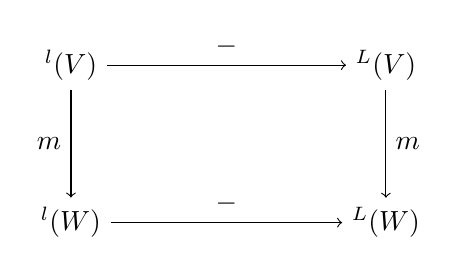
\begin{tikzpicture}[xscale=4,yscale=2]
  \node (00) at (0,0) {$\Exp^l(V)$};
  \node (10) at (1,0) {$\Exp^L(\sem{V})$};
  \node (01) at (0,-1) {$\Exp^l(W)$};
  \node (11) at (1,-1) {$\Exp^L(\sem{W})$};

  \draw[->] (00) --node[above]{$\sem{-}$} (10);
  \draw[->] (01) --node[above]{$\sem{-}$} (11);
  \draw[->] (00) --node[left]{$\ov{m}$} (01);
  \draw[->] (10) --node[right]{$\ov{\sem{m}}$} (11);
\end{tikzpicture}
\end{center}
\glec{$\ov{m}$ is the homomorphic extension of $m$, also written $\Exp^l_m$}
\end{frame}

\begin{frame}\frametitle{Substitution Theorem for translation/substitutions}
Given:
\begin{itemize}
\item formal systems $l$, $L$ with contexts and substitutions
\item a compositional translation $\sem{-}:l\to L$
\item an $l$-vocabulary $V$ and a $V$-substitution $\gamma:\Gamma\to\Delta$
\end{itemize}

\[\sem{E[\gamma]}\;\; = \;\; \sem{E}[\sem{\gamma}]\]

\begin{center}
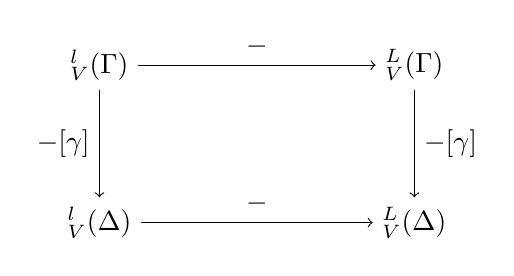
\begin{tikzpicture}[xscale=4,yscale=2]
  \node (00) at (0,0) {$\Exp^l_V(\Gamma)$};
  \node (10) at (1,0) {$\Exp^L_{\sem{V}}(\sem{\Gamma})$};
  \node (01) at (0,-1) {$\Exp^l_V(\Delta)$};
  \node (11) at (1,-1) {$\Exp^L_{\sem{V}}(\sem{\Delta})$};

  \draw[->] (00) --node[above]{$\sem{-}$} (10);
  \draw[->] (01) --node[above]{$\sem{-}$} (11);
  \draw[->] (00) --node[left]{$-[\gamma]$} (01);
  \draw[->] (10) --node[right]{$-[\sem{\gamma}]$} (11);
\end{tikzpicture}
\end{center}
\end{frame}

\begin{frame}\frametitle{Substitution Theorem for morphisms/substitutions}
Given:
\begin{itemize}
\item formal system $l$ with morphisms and contexts and substitutions
\item a morphism $m:V\to W$
\item a $V$-substitution $\gamma:\Gamma\to\Delta$
\end{itemize}

\[\ov{m}(E[\gamma])\;\; = \;\; \ov{m}(E)[\ov{m}(\gamma)]\]

\begin{center}
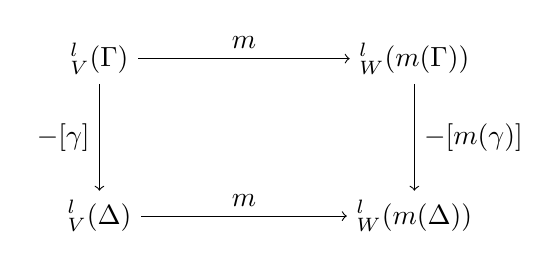
\begin{tikzpicture}[xscale=4,yscale=2]
  \node (00) at (0,0) {$\Exp^l_V(\Gamma)$};
  \node (10) at (1,0) {$\Exp^l_W(\ov{m}(\Gamma))$};
  \node (01) at (0,-1) {$\Exp^l_V(\Delta)$};
  \node (11) at (1,-1) {$\Exp^l_W(\ov{m}(\Delta))$};

  \draw[->] (00) --node[above]{$\ov{m}$} (10);
  \draw[->] (01) --node[above]{$\ov{m}$} (11);
  \draw[->] (00) --node[left]{$-[\gamma]$} (01);
  \draw[->] (10) --node[right]{$-[\ov{m}(\gamma)]$} (11);
\end{tikzpicture}
\end{center}
\end{frame}

\begin{frame}\frametitle{Substitution Theorem for the general case}
The previous cases can be seen as faces of a cube where corners are triples of language, vocabulary, context.

In general, we have
\begin{itemize}
\item formal systems $l$, $L$ with morphisms and contexts and substitutions and a compositional translation $\sem{-}:l\to L$
\item $l$-vocabularies $V$, $W$, and an $l$-morphism $m:V\to W$
\item $V$-contexts $\Gamma$, $\Delta$, and a $V$-substitution $\gamma:\Gamma\to\Delta$
\end{itemize}
and all $6$ orders of applying $\sem{-}$, $\ov{m}$, and $\gamma$ yield equal results.
\end{frame}



%\begin{frame}\frametitle{Example: Relative Computational Semantics for BOL}
%Scala, SQL semantics evaluates
%\begin{itemize}
%\item concept $c$ to
%\begin{itemize}
%\item SQL: table of individuals
% \lec{result of running query $\sem{c}$}
%\item Scala: hashset of individuals
% \lec{result of running program $\sem{c}$}
%\end{itemize}
%\item propositions to booleans \lec{accordingly}
%\end{itemize}
%
%Technically, results not in image of $\sem{-}$\\
%Fix: add productions for all values
%\begin{commgrammar}
%\gprod{F}{\true\bnfalt \false}{truth values}\\
%\gprod{C}{\{I,\ldots,I\}}{finite concepts}
%\end{commgrammar}
%\end{frame}

%
%\begin{frame}\frametitle{Equivalence of BOL Semantics}
%Now $5$ semantics for BOL
%\begin{itemize}
%\item absolute deductive via calculus
%\item relative deductive via SFOL
%\item relative computational via Scala
%\item relative concrete via SQL
%\item relative narrative via English
%\end{itemize}
%Moreover, these are interdefinable.
%\glec{e.g., Scala translation also induces deductive semantics}
%
%Can compare equivalence
%\begin{itemize}
%\item for every pair of semantics
%\item for every kind of equivalence (deductive, concrete, computational)
%\end{itemize}
%Question: Which of them hold?
%\end{frame}
%
%\begin{frame}\frametitle{Questions}
%For example, consider:
%\begin{itemize}
%\item Are the absolute semantics and the Scala semantics deductively equivalent?
%\item Assuming BOL and SQL have the base types and values:
%Are the absolute semantics and the SQL semantics concretely equivalent?
%\end{itemize}
%\end{frame}
%
%
%\begin{frame}\frametitle{Computational Semantics of BOL}
%Are these two BOL semantics deductively equivalent
%\begin{itemize}
%\item absolute deductive semantics 
%\item relative deductive semantics via translation $\sem{-}$ to Scala
%\end{itemize}
%
%\only<1>{
%Soundness: $\vdash^{BOL}_V f$ implies $\vdash^{Scala}_{\sem{V}}\sem{f}\rewrites \true$
%\begin{itemize}
%\item Problem: Absolute semantics performs consequence closure, e.g.,
%\begin{itemize}
%\item transitivity of $\sqsubseteq$
%\item relationship between $\sqsubseteq$ and $\isa$
%\end{itemize}
%\item Scala semantics does so only if we explicitly implemented it
%\glec{we didn't}
%\glec{same problem for SQL semantics}
%\end{itemize}
%}
%
%\only<2>{
%Completness: $\vdash^{BOL}_V f$ implied by $\vdash^{Scala}_{\sem{V}}\sem{f}\rewrites \true$
%\begin{itemize}
% \item absolute semantics leaves closed world optional
% \item Scala uses closed worlds
%  \glec{e.g., used to compute $c\sqsubseteq d$ by checking all individuals} 
% \item complete only if we add induction rule
%\end{itemize}
%}
%\end{frame}


\end{document}

